\section{Background Predictions \label{BackPred}}
All of the analyses count the number of tracks passing threshold values on some grouping of the $p_T$, \invbeta, 
and \ias\ variables. The \tktof\  and \tkonly\ analyses also place a requirement on the mass of the track as described below. There are two sources
of background considered in the analyses. 

The first is muons, or for the \tkonly\ analysis any charged SM particle, from the collisions in the LHC. Muons can pass the thresholds on the selection variables
for a variety of reasons.
All muons at the LHC will be traveling at very nearly the speed of light,
but finite detector resolution results in a smearing of the measured time of hits. This can cause muons to have a high measured \invbeta.
While muons in the momentum region of interest all deposit approximately
the same amount of energy in the tracker on average, the amount deposited in each interaction is subject to large variations. This can lead to muons
with a high \dedx\ value. Detector resolution can also contribute to muons with high \dedx.
Additionally, collision muons can have large reconstructed momentum, either due to true high momentum or detector mismeasurement
promoting a low momentum muon to a high reconstructed momentum. Detector mismeasurement is especially important for the momentum measured in the muon system.

The number of collision muons to pass the thresholds is predicted by exploiting the lack of correlation between the selection variables for muons through the $ABCD$ method.
In the $ABCD$ method, multiple bins are defined by whether the track passes thresholds on the selection variables. In the normal two dimensional version
of the $ABCD$ method, two selection variables are used and four regions are defined. The $A$ region has tracks failing both of the thresholds on the selection
variables, the $B$ ($C$) region fails only the threshold on the first (second) of the selection variables, and the $D$ region,
the signal region, passes the threshold on both selection
variables. The number of background muons in the $D$ region can be predicted as $B \times C / A$, where the letters represent the number of tracks in the regions.
This prediction holds as long as the probability for a background
muon to pass the threshold on one of the variables is independent of whether it passes the threshold of the other. Tests of the correlation between the selection variables are
discussed below.

The four different analyses use different combinations of the selection variables defined in Sec.~\ref{sec:SelVar}. 
With three different selection variables (\pt, \invbeta, \dedx), eight different bins are defined.
In order to simplify the nomenclature in this section, Table~\ref{tab:BinNames} 
defines the names of the bins (ranging from $A$-$H$) and whether they pass or fail the thresholds on the selection variables. For all
the selection variables passing means having a value above the threshold. If a selection variable
is not used in an analysis then it is taken to have passed. 

Only the \tktof\ analysis applies a threshold on all three selection variables, and as such is the only one to use all eight bins.
An extended three-dimensional version of the $ABCD$ method is then used to make the prediction as is described in the \tktof\ subsection below.
The other three analyses use only the four bins where the unused variable is said to have passed. These analyses use the traditional two-dimensional $ABCD$ method
though the names of the bins may be different.
For all the analyses the D region is always the signal region. 

In order to perform systematic studies, the analyses that use \invbeta\ reverse the preselection requirement on \invbeta\ greater than one. This creates a group of tracks
measured as going faster than the speed of light, making it signal free. As the \invbeta\ distribution is close to symmetrical for background muons,
this region is very good for testing the background prediction. New bins are defined as in Table~\ref{tab:BinNames} but now \invbeta\ is said to have passed
if the value is below the threshold. The bins are referred to with a prime to denote that they are from the control region, so the new ``signal'' region would
be referred to as $D^{\prime}$.


\begin{table}
 \begin{center}
  \caption[Bin naming convention for background regions]
{Bin naming convention.  The signal region is always the D region.}
     \label{tab:BinNames}
  \begin{tabular}{|c|c|c|c|} \hline
   Name & $p_T$ & \invbeta\   & \ias\  \\ \hline
   A    & Fail      & Fail            & Pass           \\ \hline
   B    & Fail      & Pass            & Pass           \\ \hline
   C    & Pass      & Fail            & Pass           \\ \hline
   D    & Pass      & Pass            & Pass           \\ \hline
   E    & Fail      & Fail            & Fail           \\ \hline
   F    & Fail      & Pass            & Fail           \\ \hline
   G    & Pass      & Fail            & Fail           \\ \hline
   H    & Pass      & Pass            & Fail           \\ \hline
  \end{tabular}
 \end{center}
\end{table}

The second source of background, important only for the \muononly\  analysis,
%and \fract\ analyses, 
is muons from cosmic-rays. 
As discussed in Section~\ref{sec:SM} muons from cosmic-rays
are constantly passing through CMS. Cosmic-ray muons will arrive to the muon system asynchronously with collisions in the LHC. Depending on exactly
when the cosmic-ray muon arrives in the muon system relative to collisions in the LHC this can give rise to a particle with a large \invbeta\ measurement.
The distribution of $p_T$ for cosmic-ray muons falls off at high momentum slower than for collision muons, as evidenced in Figure~\ref{fig:MuOnlySelVar} (left).
As cosmic-ray muons have different \invbeta and \pt\ distributions than collision muons they will not be accurately predicted with the same method used to predict
the collision-muon background in the \muononly\ analysis. A dedicated method using the cosmic-ray muon control sample is described below.

Cosmic-ray muons are not a background for the analyses that look for high-ionizing tracks as
out-of-time particles are not centered in the tracker's charge collection window.
This results in only a portion of their ionization energy loss being collected and their reconstructed \dedx\ being smaller than a collision muon.
Thus, cosmics have the signature of anomalously low reconstructed \dedx~\cite{CMS:2012xi}, opposite of the signature for an HSCP.
Additionally, the impact parameter cuts applied on the tracker track greatly reduce the number of cosmic-ray muons passing the preselection.
Either of these requirements on their own is enough to make the cosmic-ray muon background very small for the analyses looking for high \dedx\ in the tracker,
with both applied the background is completely negligible.

For all the analyses, the expected background in the signal region is estimated by multiple different predictions.
The details on how the different predictions are found for each analysis are given in the corresponding subsection below.
The spread of the different background predictions can be used to estimate the systematic uncertainty for each analysis.

The following variables are defined:
\begin{equation}
\centering
\begin{split}
S^{syst+stat}_{N} &= \sqrt{\sum_i \left( x_i - \langle x \rangle  \right) ^2/(N-1)} \\
S^{stat}_{N} &= \sqrt{\sum_i \left( \sigma _i \right) ^2/N} \\
S^{syst} &= \sqrt{S_{syst+stat}^2-S_{stat}^2} \\
\end{split}
\label{eq:variance}
\end{equation}
where N is the number of background estimates made,
the sum is over N, $x_i$ is the value of the $i^{th}$ background estimate,
and $\sigma_i$ is the statistical uncertainty on
the $i^{th}$ background estimate. The first quantity is an estimator of the
standard deviation of the background estimates, which takes both statistical
and systematic contributions. The second quantity is adopted as an
estimator of the contribution of the statistical uncertainties
to the standard deviation. Finally, the last equation gives the systematic uncertainty on the background prediction assuming
the statistical and systematic uncertainties add in quadrature to give the standard deviation.

\subsection{Prediction for \muononly\ analysis \label{sec:MuOnlyPred}}

The collision muon  background in the \muononly\ analysis is predicted with the selection criteria of \invbeta\ and \pt\ in the $ABCD$  method.
%by exploiting the lack of correlation between the selection variables for background particles. 
The expected number of background tracks in the signal region $D$ (see Table~\ref{tab:BinNames}) is predicted as $B \times C / A$. 
%Tracks are divided into four groups based on whether they
%have $p_T$ and \invbeta\ values greater than the thresholds placed on these selection criteria. 
%The four groups are referred to as $A$,$B$,$C$, and $D$. The $A$ group contains tracks that have $p_T$ and \invbeta\ values lower than both selection thresholds
%while the $B$($C$) group contains tracks that have only the $p_T$ (\invbeta) below its threshold. The groups containing the tracks with \invbeta\
%below the its threshold only contains tracks with $1 < $\invbeta\ $< $ threshold. Tracks with \invbeta\ $< 1$ are used to evaluate how well the prediction performs.
%The $D$ group contains tracks passing both thresholds and is considered the signal region. 

%The predicted number of collision muons in the signal region is found via the relation $B \times C / A$. This relation is accurate so long as the ratio of tracks
%passing the \invbeta\ cut is the same regardless of whether the $p_T$ cut is passed, the statement is also true reversing the roles of \invbeta\ and $p_T$.
The $ABCD$ method only works if the probability to pass one of the thresholds is independent of the other variable.
However, it has been observed that a correlation exists between the $p_T$ and \invbeta\ measurements based on whether the track is in the barrel or forward
region of the detector as well as the number of DT or CSC stations containing valid hits. 
Six bins are created defined by the $\eta$ of the track, greater or less than 0.9; and the number of stations, 2, 3, or 4.
The distributions of \pt\ and \invbeta\ in the six regions is shown in Figure~\ref{fig:SelVarBinned}.
The predicted number of tracks in each bin is predicted separately and the total number of predicted background tracks is the sum of the six predictions.

\begin{figure}
\centering
  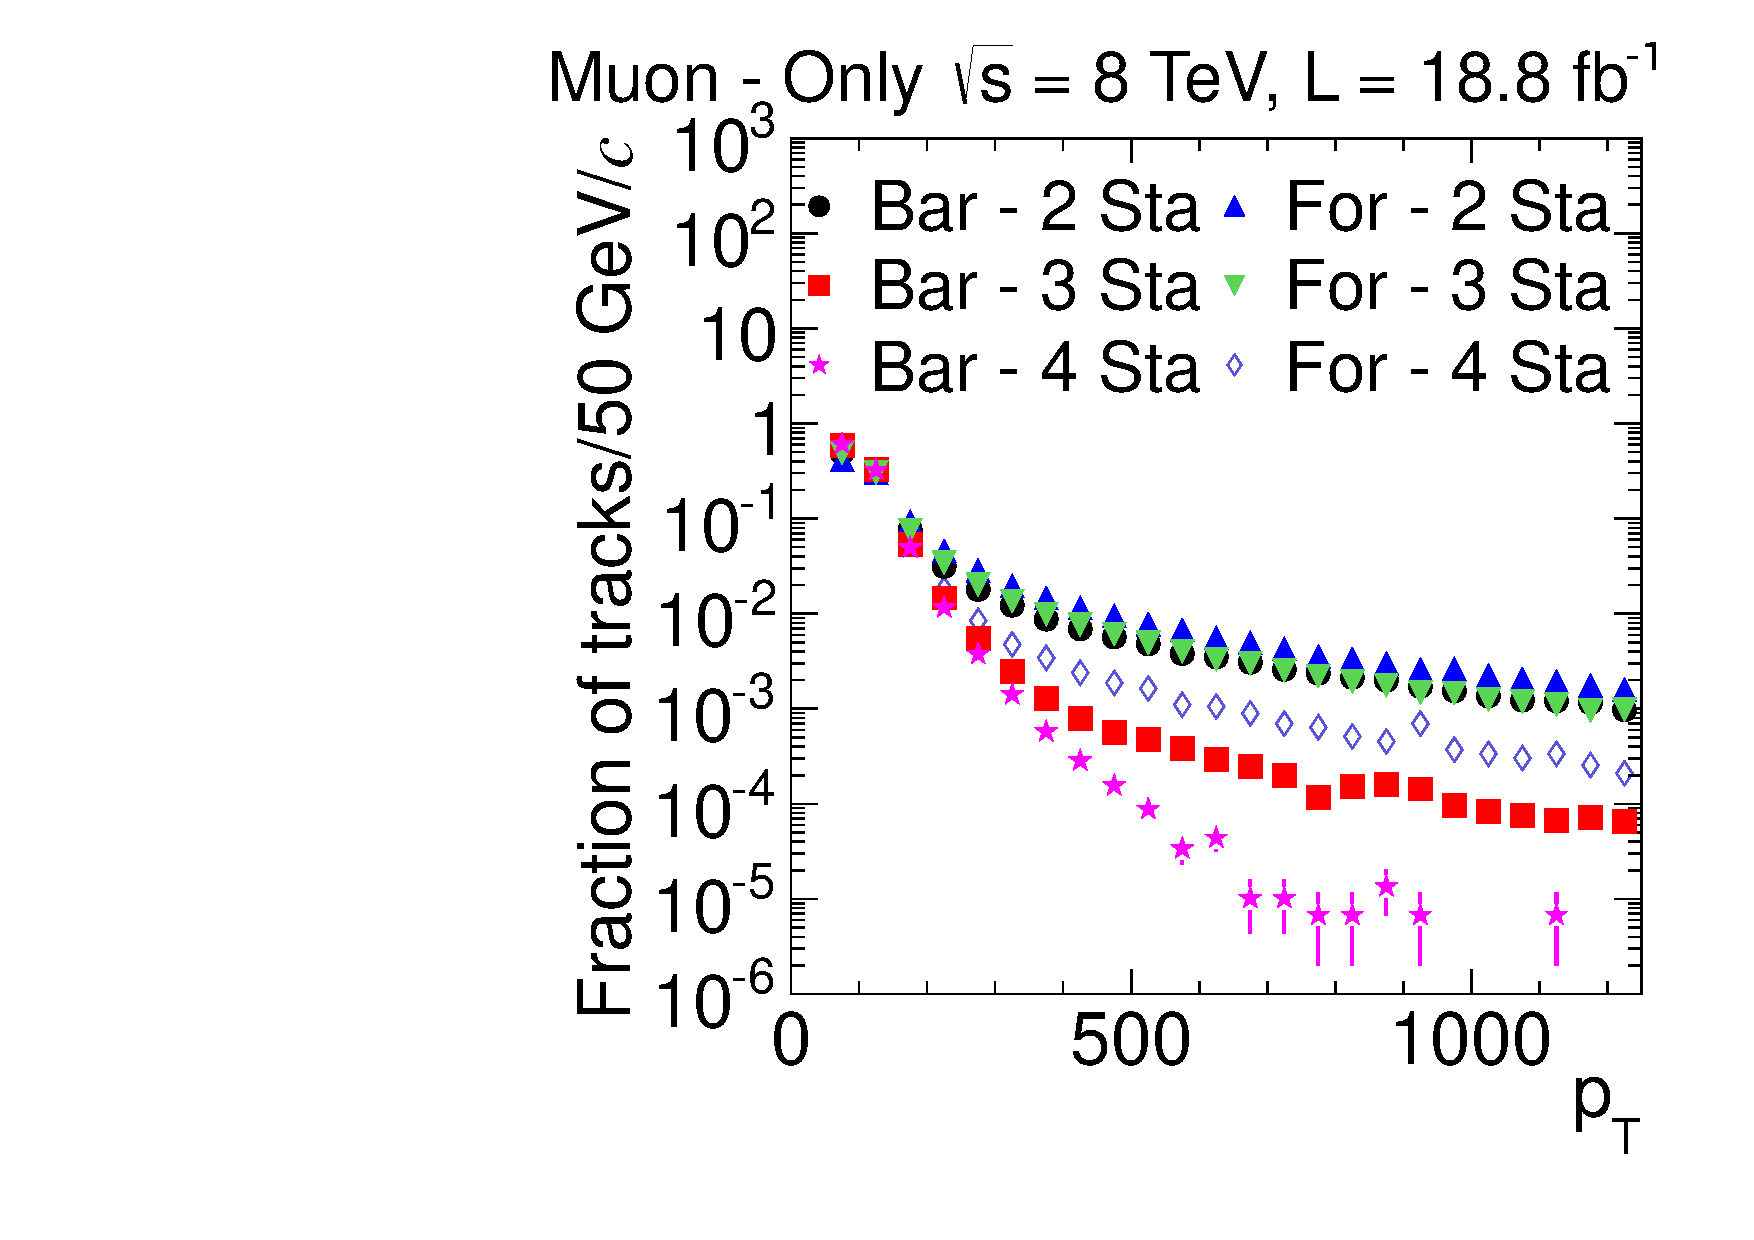
\includegraphics[clip=false, trim=0.0cm 0cm 0.0cm 0cm, width=0.48\textwidth]{figures/muonly/Selection_Data8TeV_Pt_Binned_BS}
  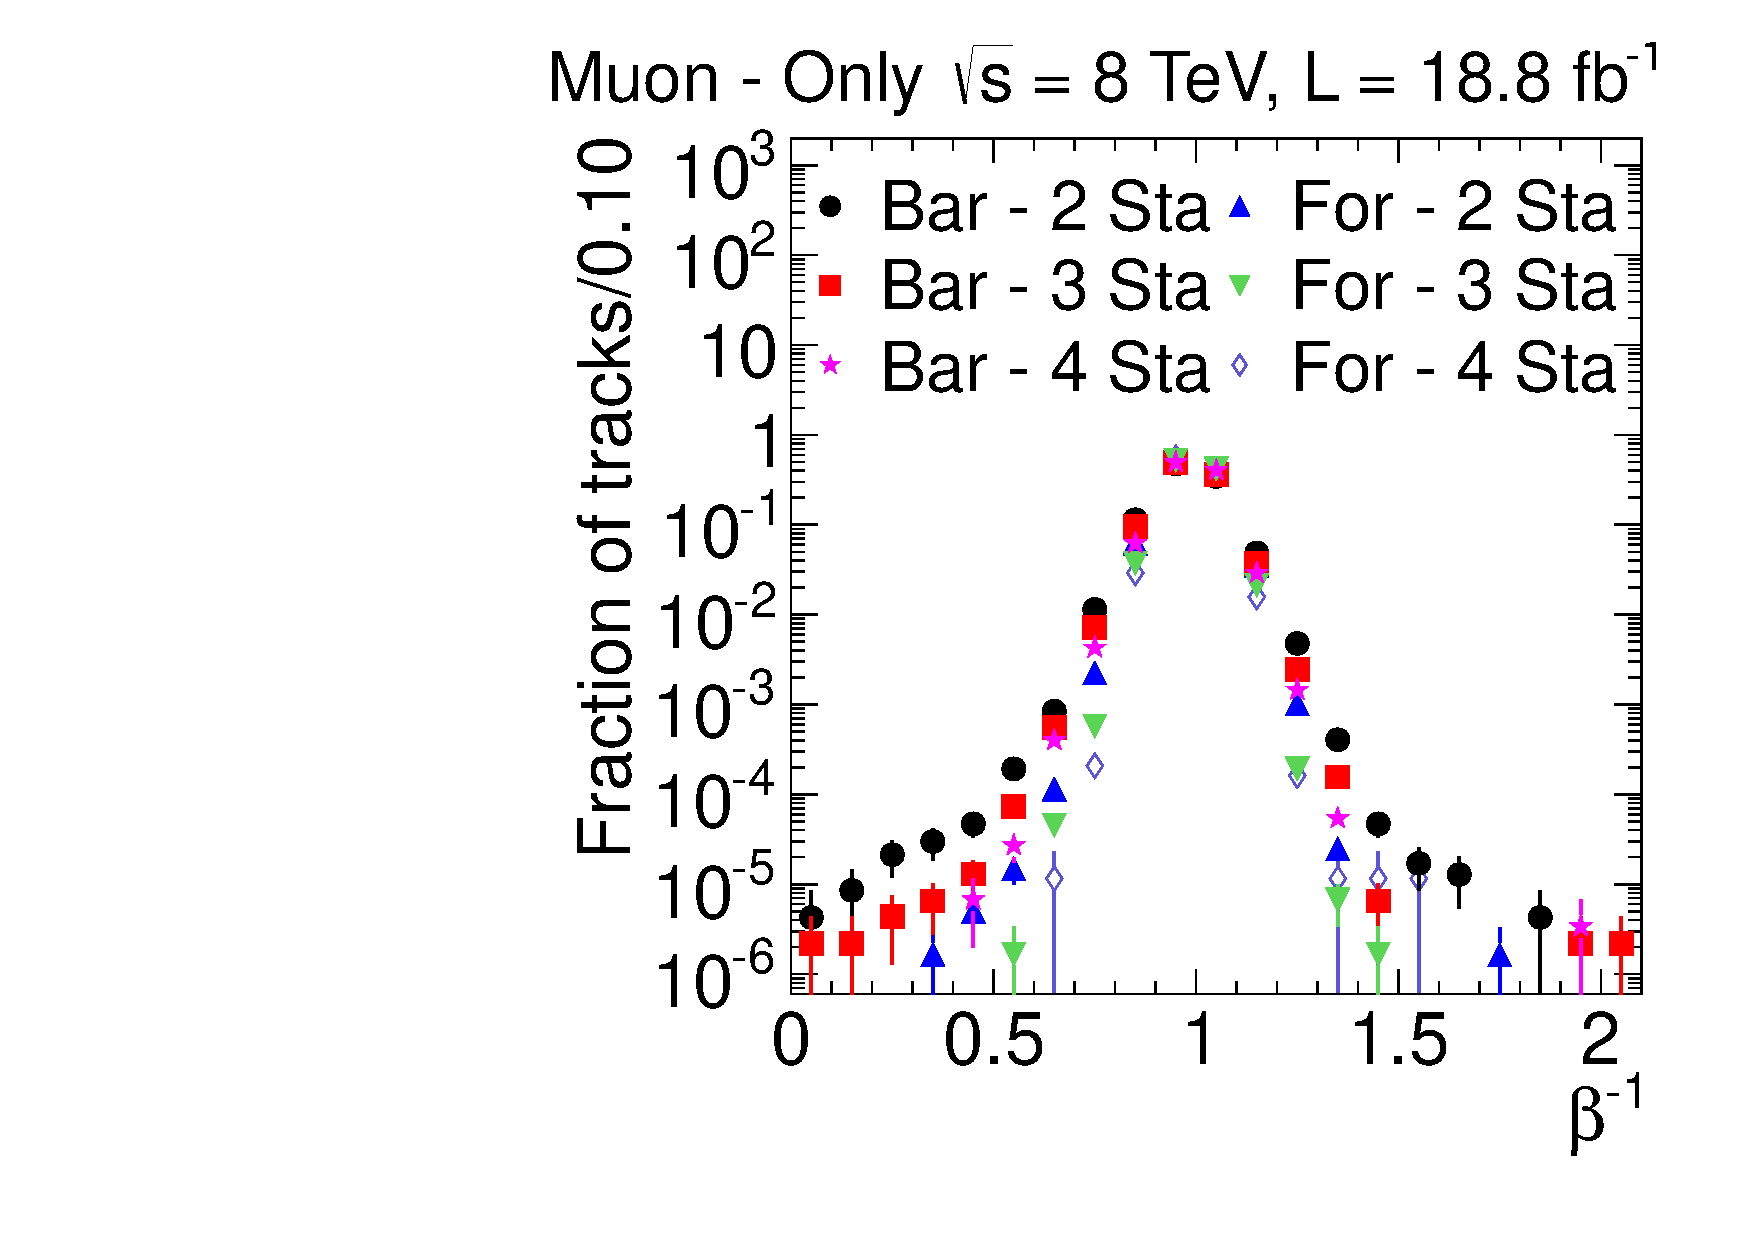
\includegraphics[clip=false, trim=0.0cm 0cm 0.0cm 0cm, width=0.48\textwidth]{figures/muonly/Selection_Data8TeV_TOF_Binned_BS}
\caption[Distribution of $p_T$ and \invbeta\ for data in different prediction regions in the \muononly\ analysis]
{Distribution of $p_T$ and \invbeta\ for data for six different regions depending on whether the track is in the barrel (Bar)
or forward (For) region of CMS and number of muon stations (Sta) used in the fit.}
    \label{fig:SelVarBinned}
\end{figure}

After the binning the correlation is small enough not to bias the background prediction as can be seen in Figs.~\ref{fig:MuOnlyControl} and~\ref{fig:MuOnlyControl4}.

\begin{figure}
\begin{center}
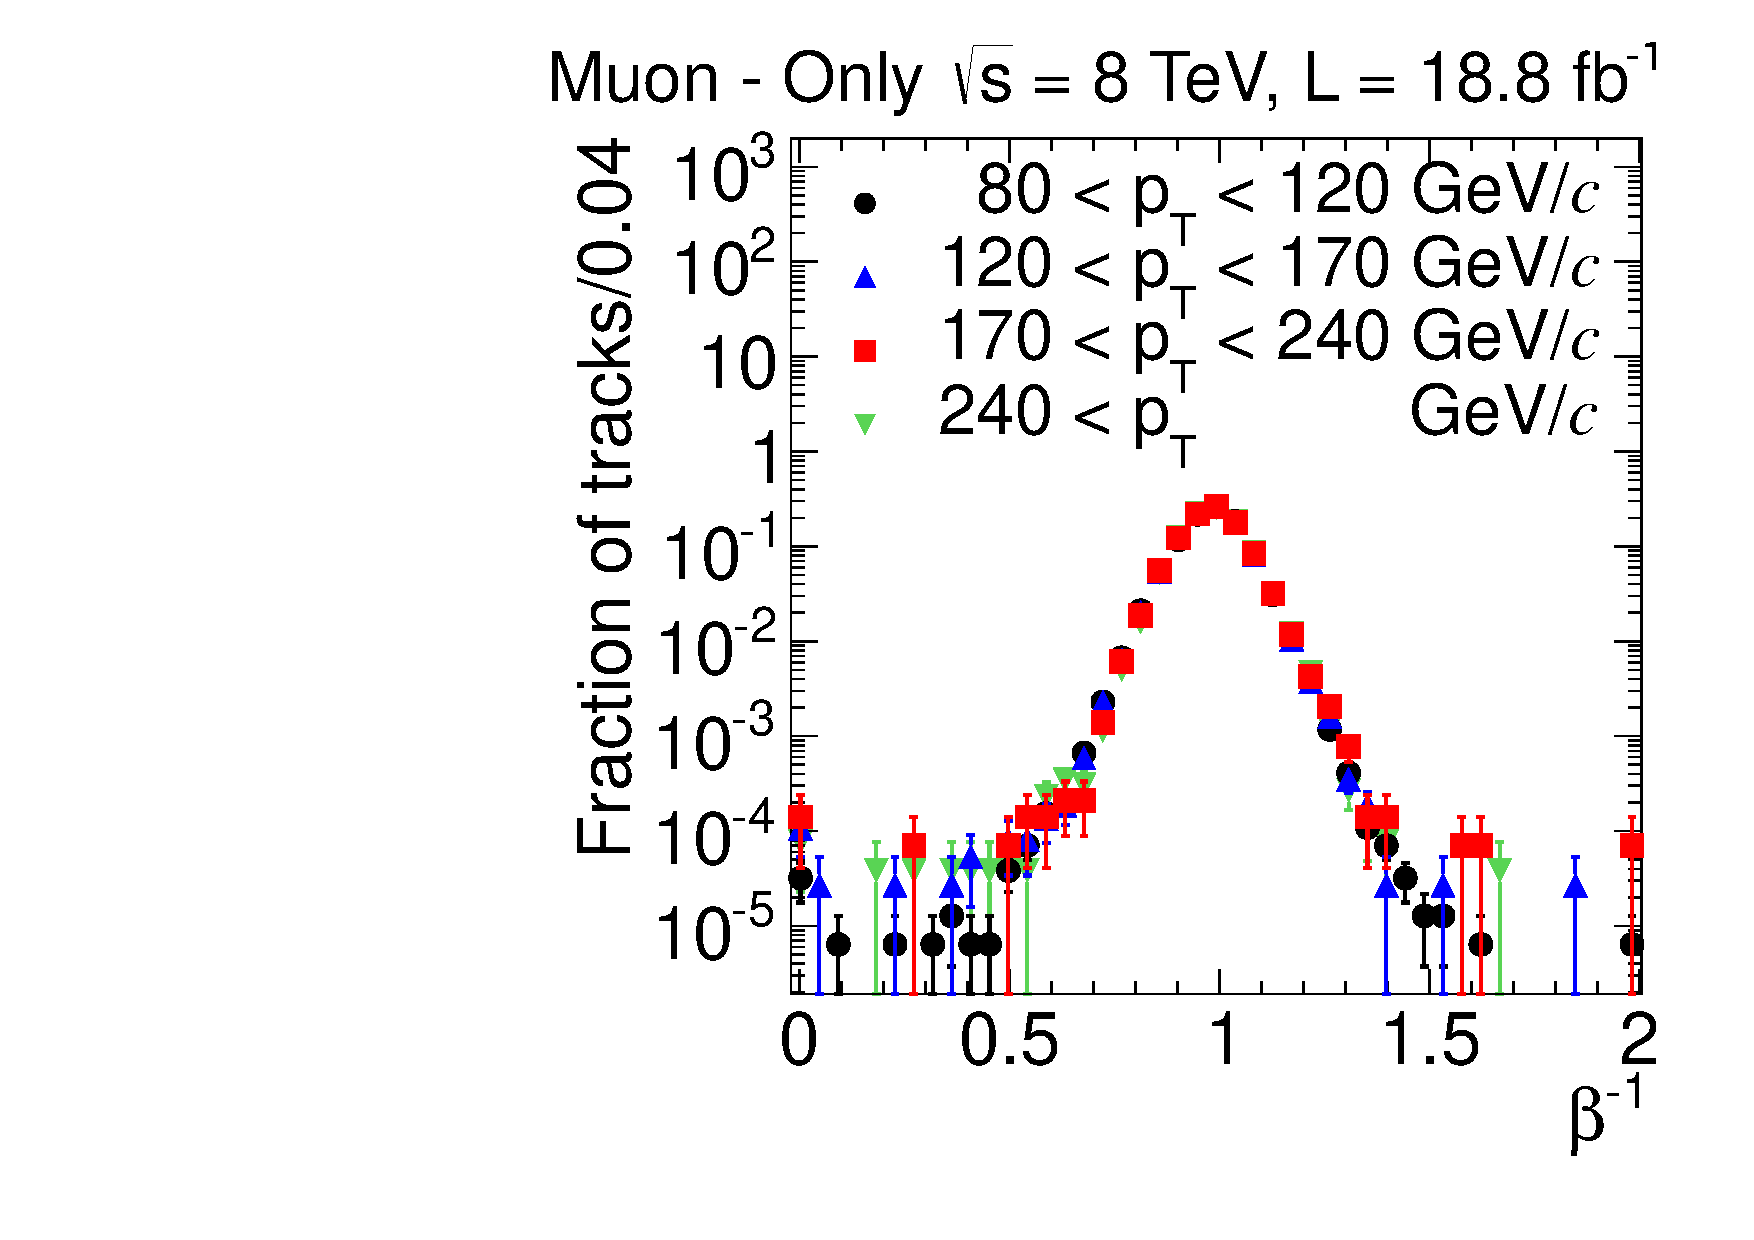
\includegraphics[clip=false, trim=0.0cm 0cm 0.0cm 0cm, width=0.48\textwidth]{figures/muonly/Control_Data8TeV_Pt_TOFSpectrum_Binned_0}
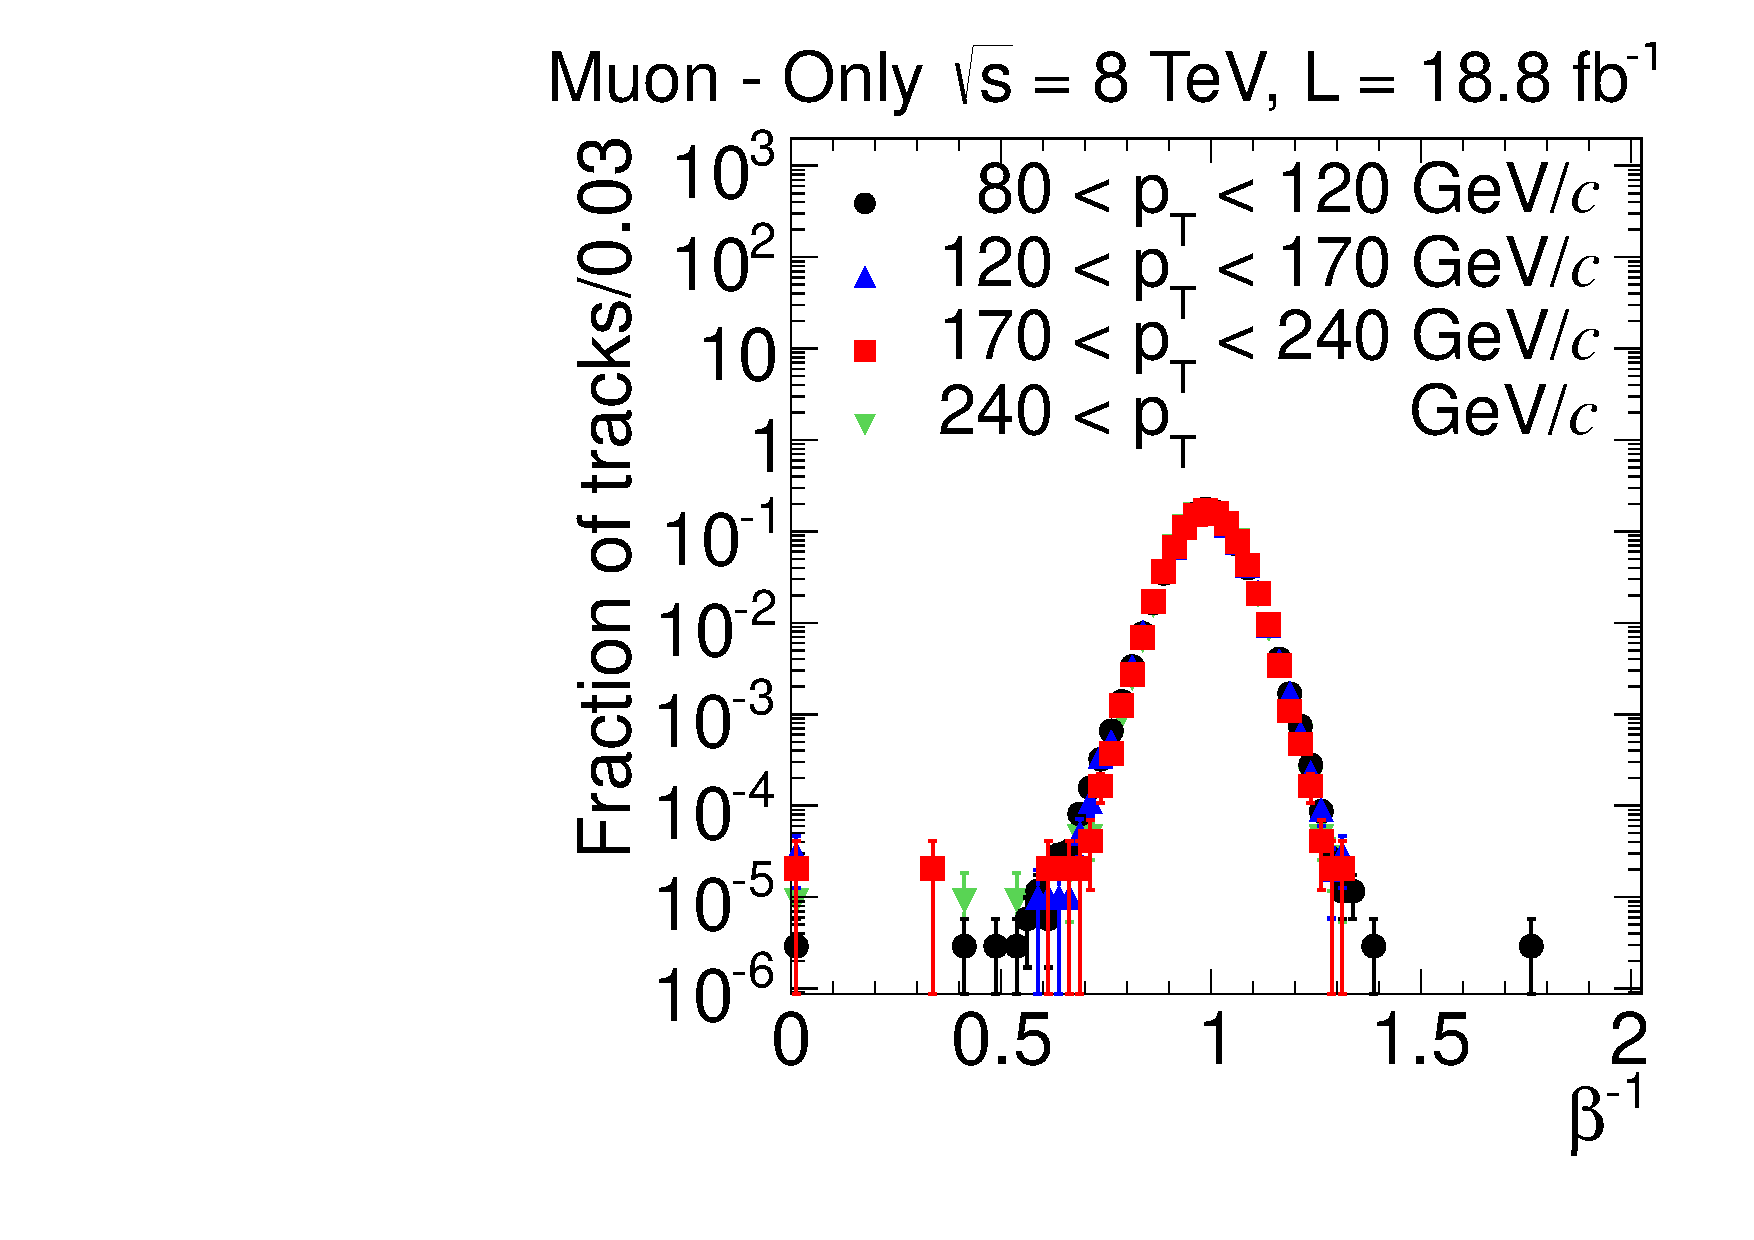
\includegraphics[clip=false, trim=0.0cm 0cm 0.0cm 0cm, width=0.48\textwidth]{figures/muonly/Control_Data8TeV_Pt_TOFSpectrum_Binned_3} \\
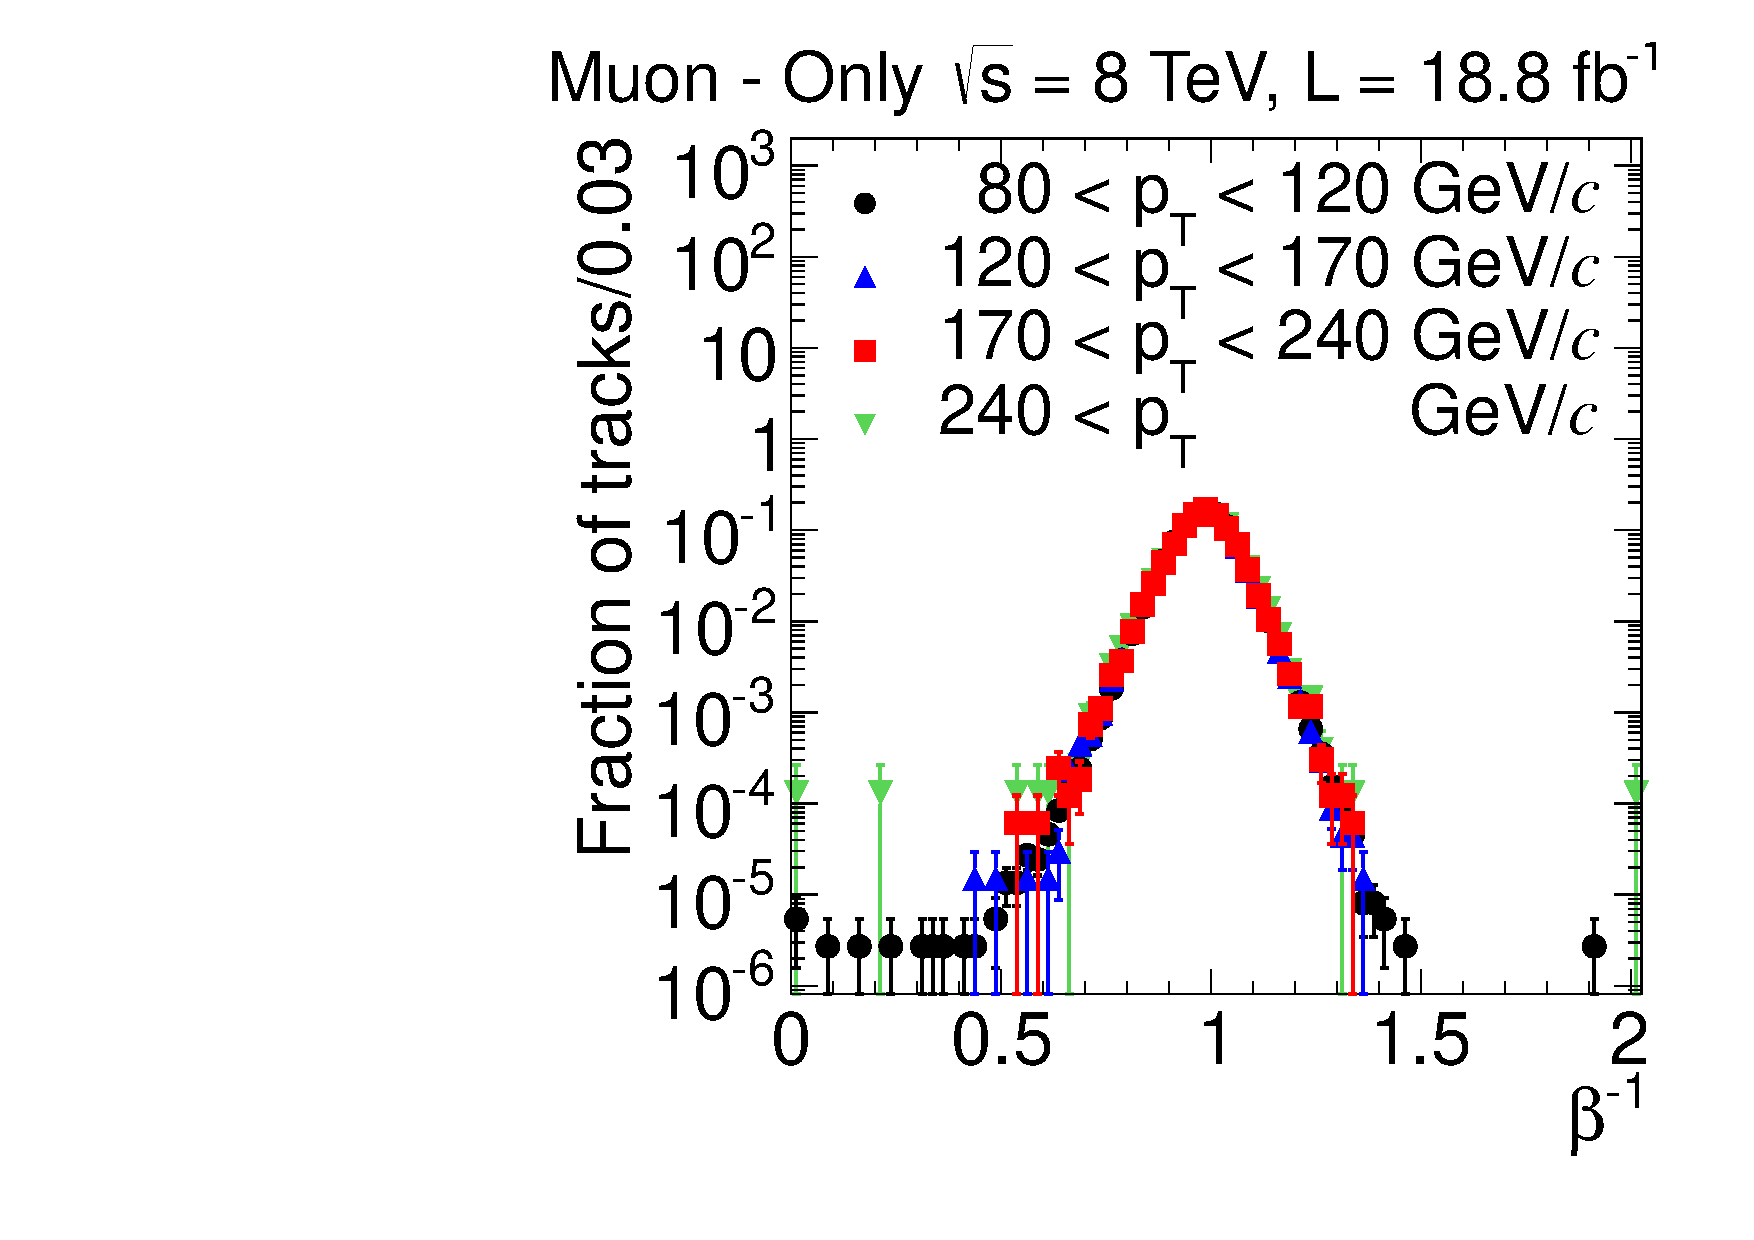
\includegraphics[clip=false, trim=0.0cm 0cm 0.0cm 0cm, width=0.48\textwidth]{figures/muonly/Control_Data8TeV_Pt_TOFSpectrum_Binned_1}
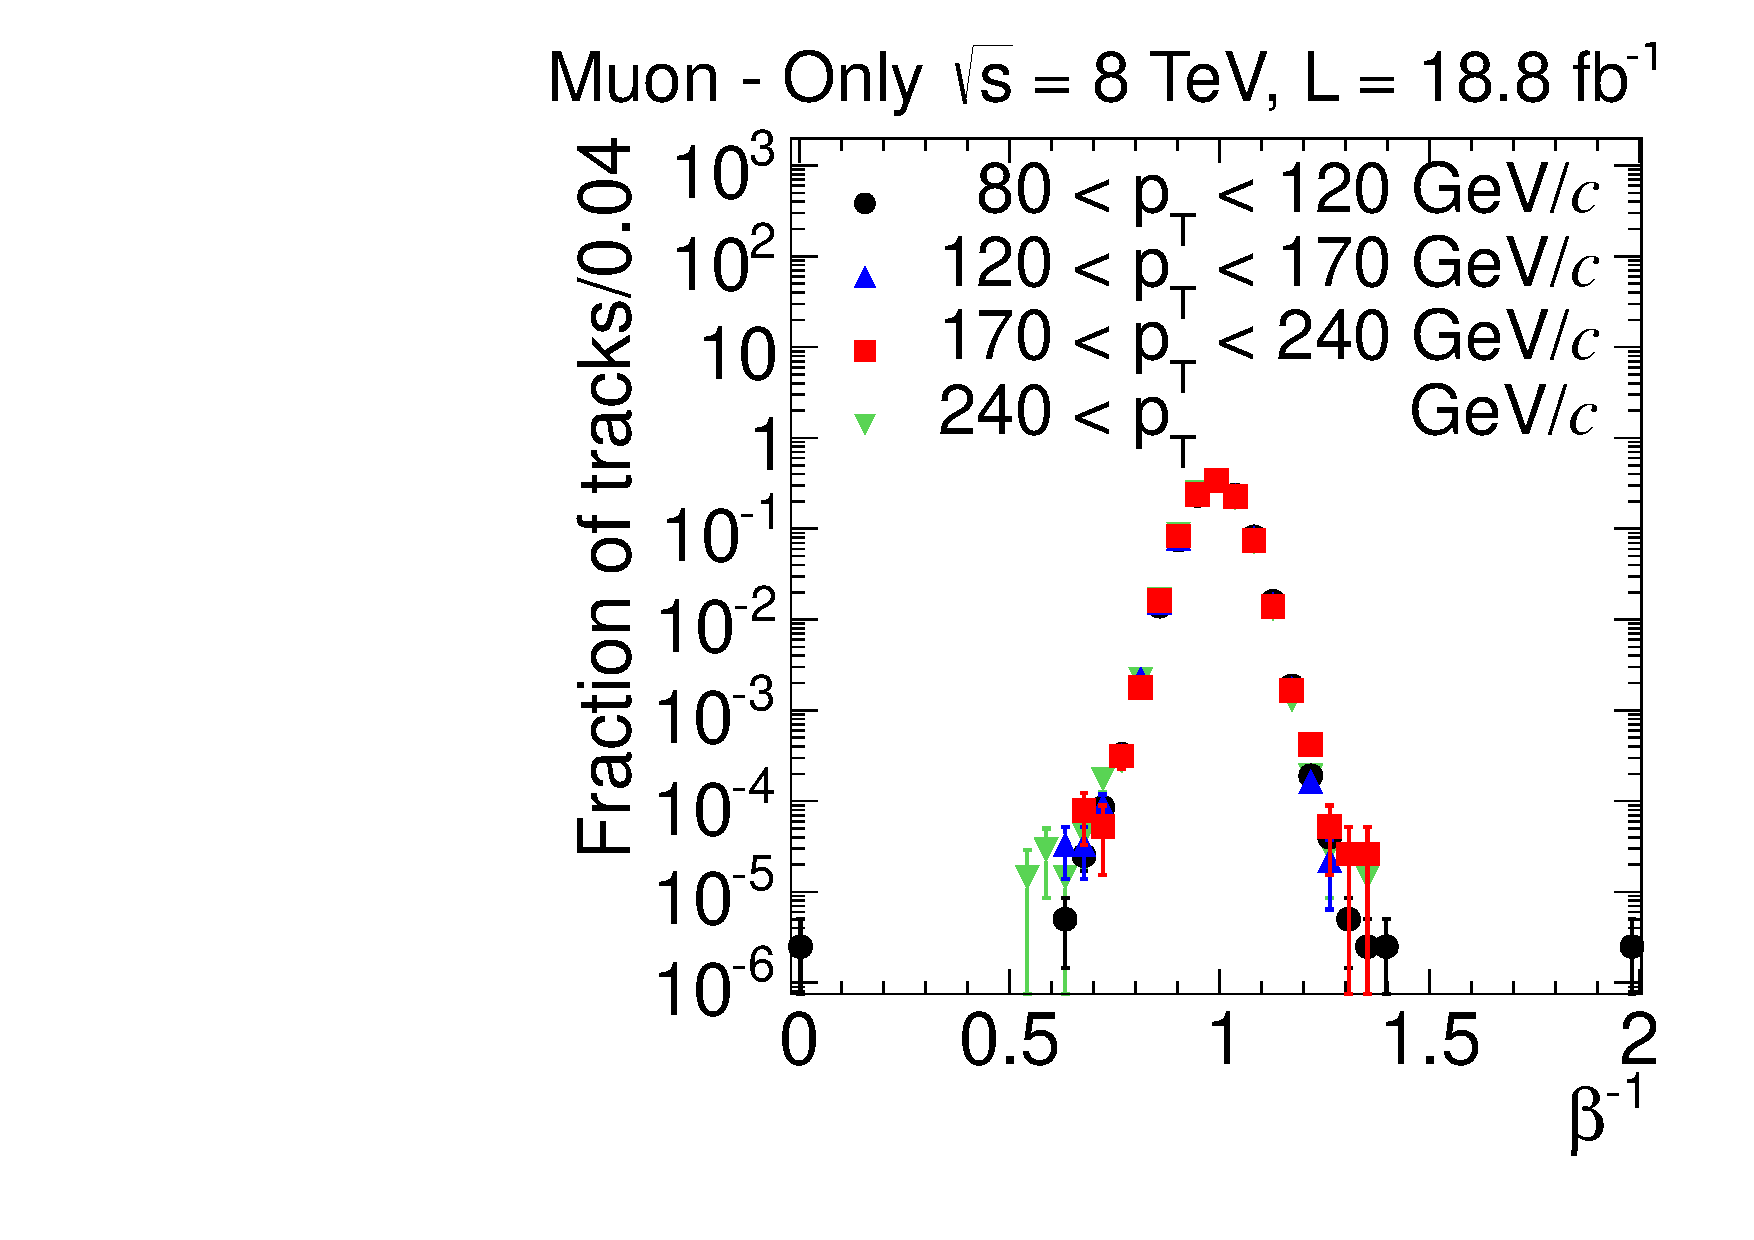
\includegraphics[clip=false, trim=0.0cm 0cm 0.0cm 0cm, width=0.48\textwidth]{figures/muonly/Control_Data8TeV_Pt_TOFSpectrum_Binned_4}
\caption[Distribution of \invbeta\
for different momentum regions for two and three station tracks in the \muononly\ analysis.]
{Distribution of \invbeta\ 
for different momentum regions for four of the six different bins that are used to make the prediction.
The left column shows the barrel region while the right column
shows the forward region.  The top (bottom) row are for 2 (3) stations.}
\label{fig:MuOnlyControl}
\end{center}
\end{figure}

\begin{figure}
\begin{center}
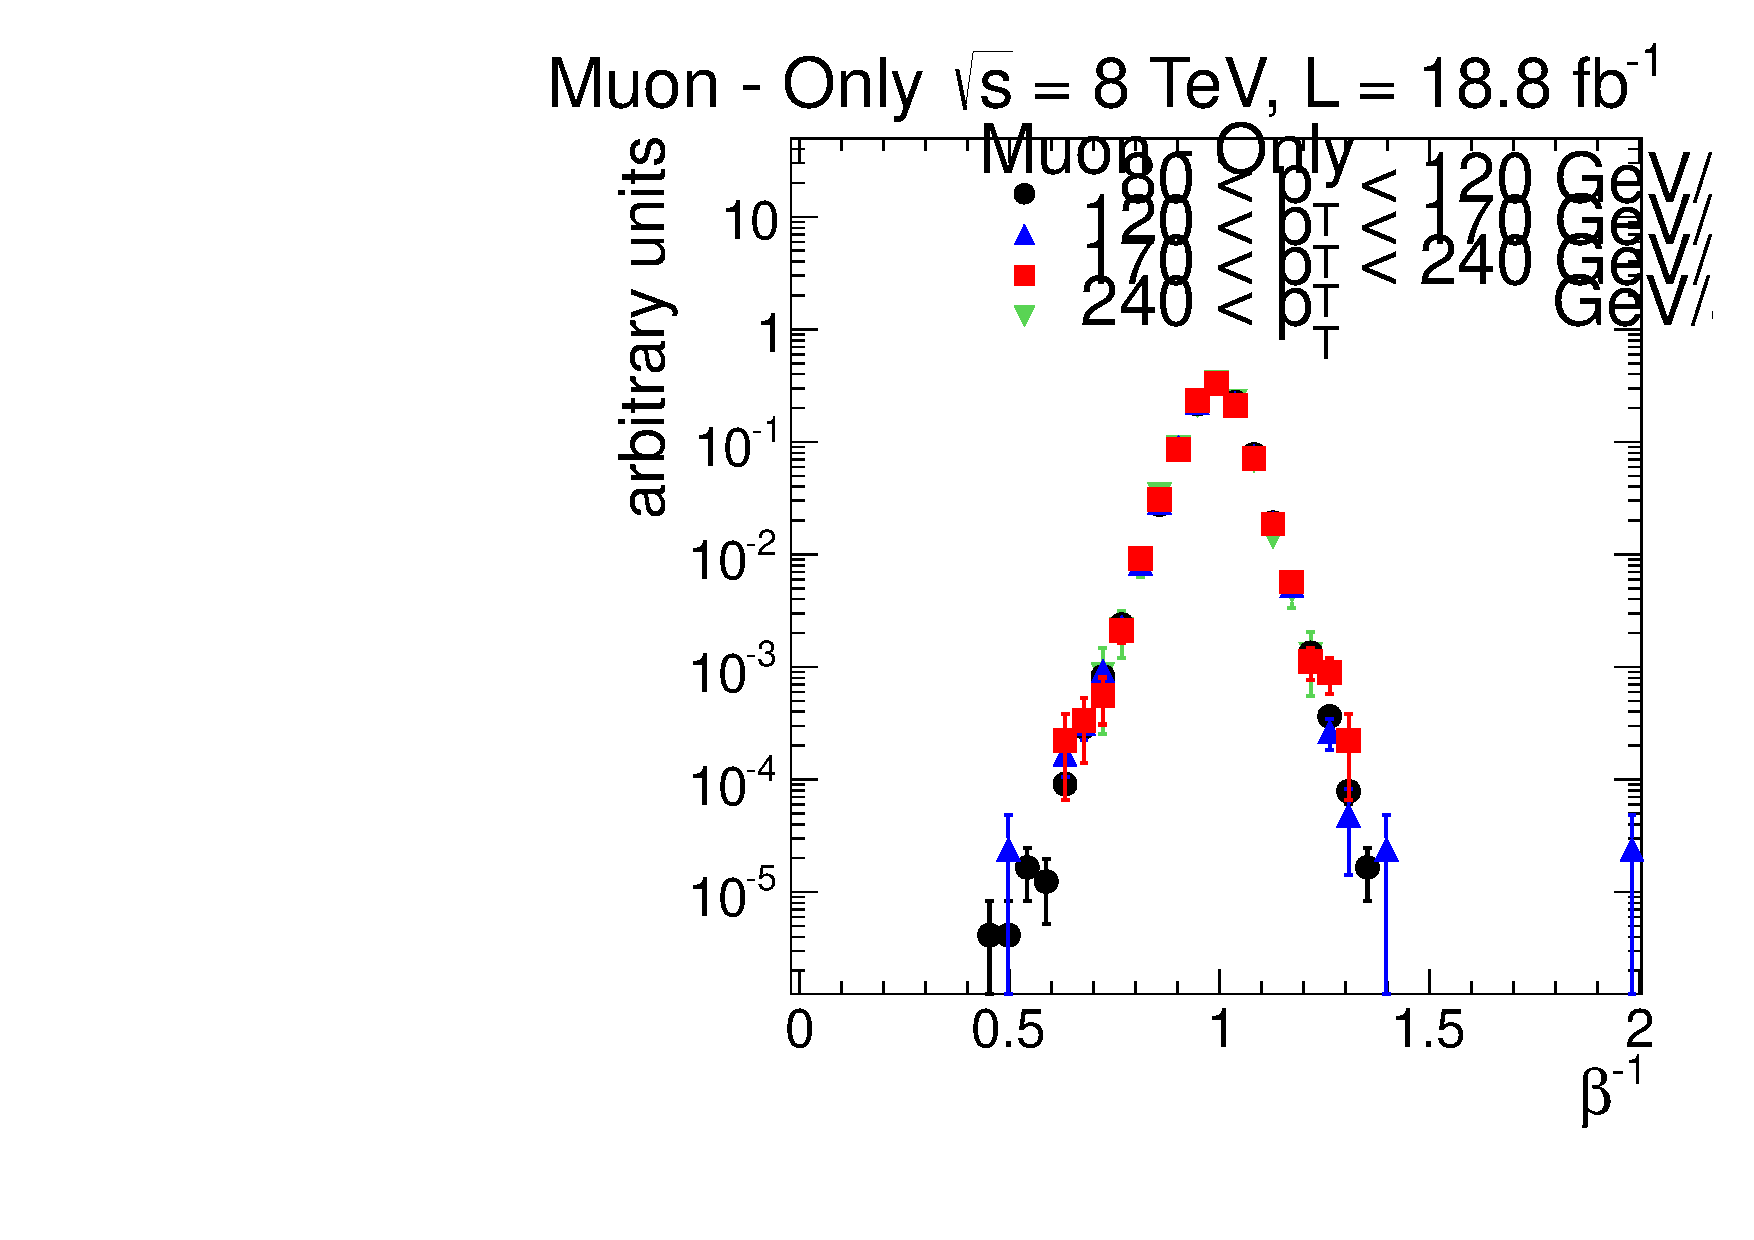
\includegraphics[clip=false, trim=0.0cm 0cm 0.0cm 0cm, width=0.48\textwidth]{figures/muonly/Control_Data8TeV_Pt_TOFSpectrum_Binned_2}
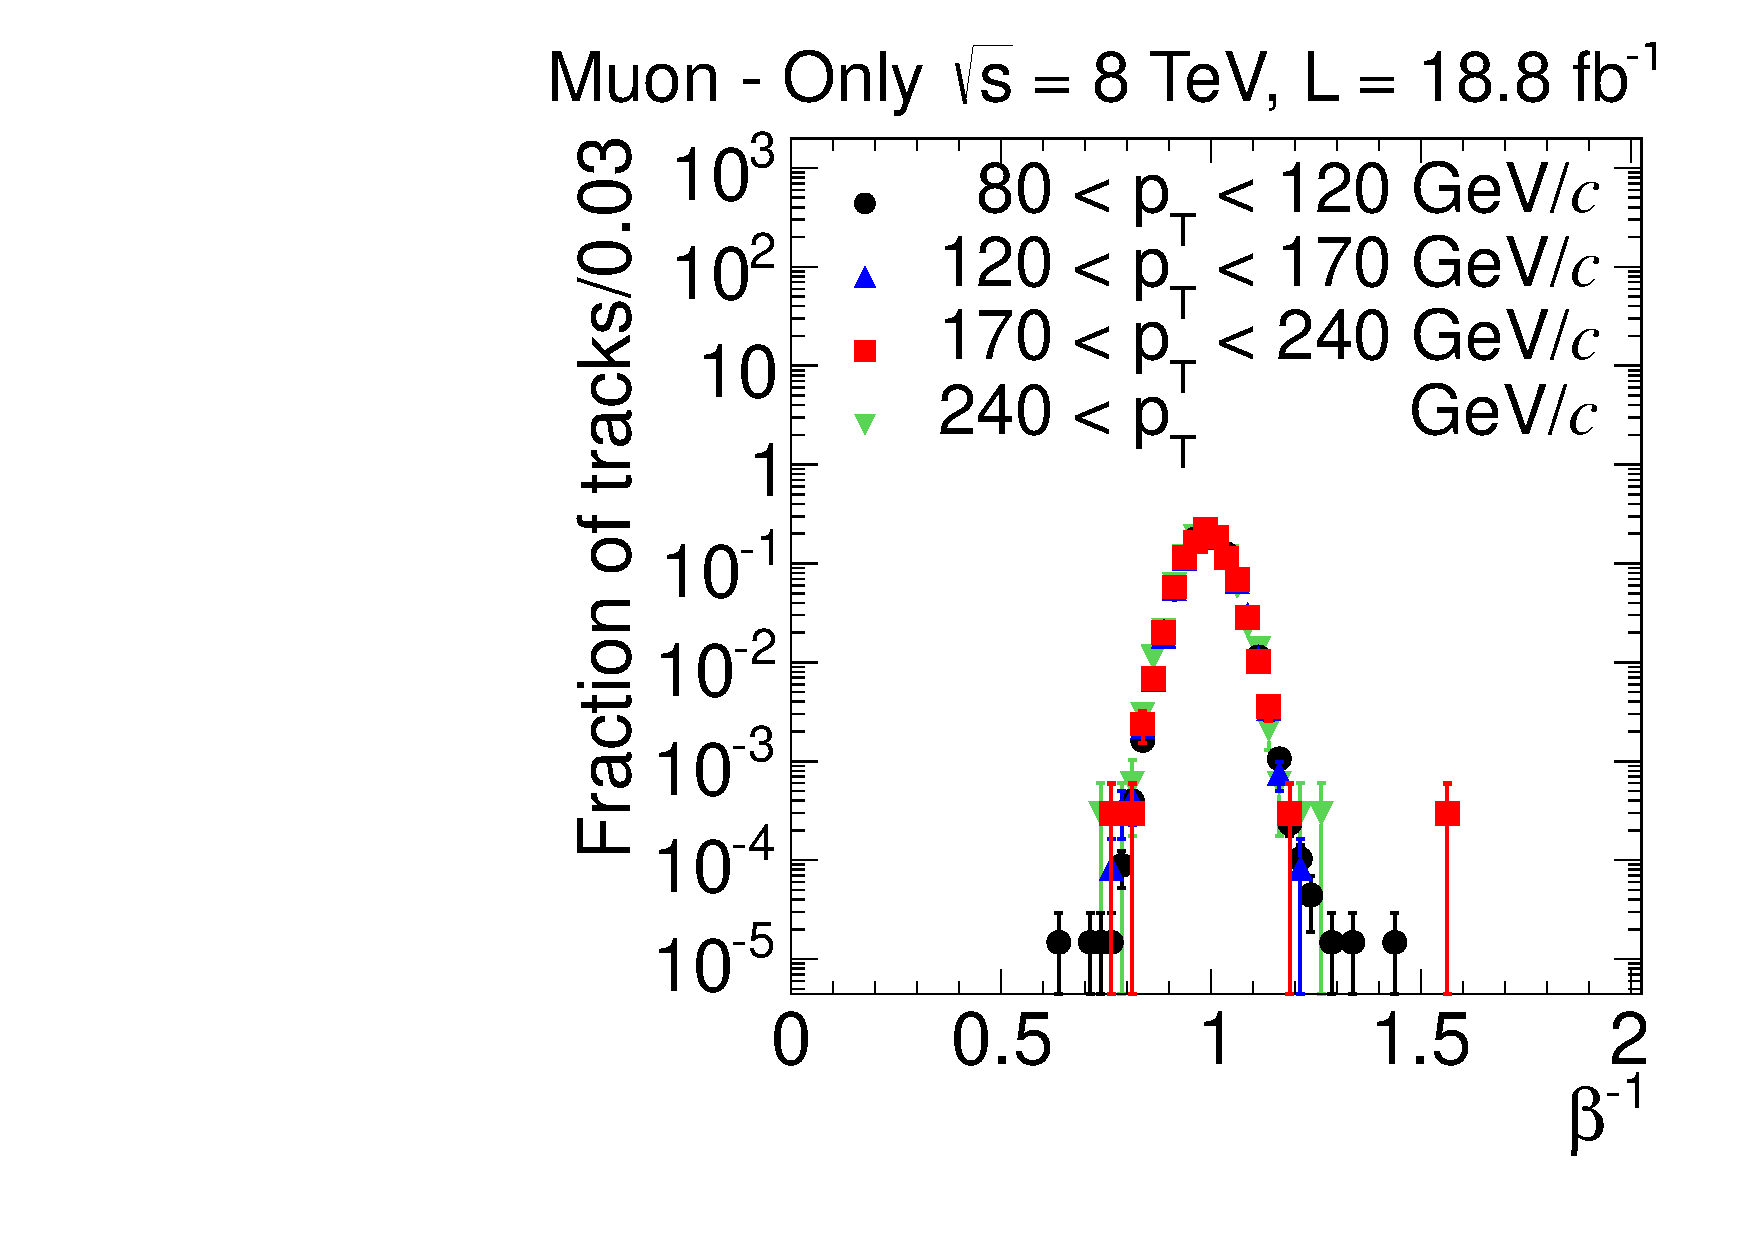
\includegraphics[clip=false, trim=0.0cm 0cm 0.0cm 0cm, width=0.48\textwidth]{figures/muonly/Control_Data8TeV_Pt_TOFSpectrum_Binned_5}
\caption[Distribution of \invbeta\
  for different momentum regions for four station tracks in the \muononly\ analysis.]
{Distribution of \invbeta\
for different momentum regions for four station tracks.
The  left column shows the barrel region while the right column
shows the forward region.}
\label{fig:MuOnlyControl4}
\end{center}
\end{figure}

To predict the cosmic-ray-muon background, sidebands in the $|\delta_z|$ distribution and the pure cosmic-ray muon sample (see Section~\ref{sec:samples}) are used.
The number of tracks, $N$, in a sideband region of $|\delta_z|$ are counted. The tracks are required to pass the full selection except the $|\delta_z|$ requirement 
is changed from $0 < |\delta_z| <$~15~cm to $70 < |\delta_z| <$~120~cm and
the requirements on $\phi,$ segment $\eta$ separation, and $p_T$ are removed to increase the number of cosmic-ray muons in the sideband region. 
Additionally the tracks
are required not to be reconstructed in the silicon tracker to decrease the contamination from collision muons. 
Then, the pure cosmic-ray sample is used to calculate the ratio, $R$, of tracks in the $|\delta_z|$ sideband region 
relative to the signal region with the same offline requirements as in the main data sample. 

The number of cosmic-ray muons passing the final selection in the main data sample can then be predicted as 
\begin{equation}
\begin{split}
P_{Cosmic} = N \times R.
\end{split}
\label{eq:CosmicPred}
\end{equation}
Numerous effects cancel in this ratio, making the prediction robust. The number of cosmic-ray muons in any of the regions can be expressed as 
$C = F \times T \times \epsilon$, where C is the number of cosmic-ray muons observed, F is the flux of cosmic-ray muons per second, T is the amount of time that CMS was collecting data, and $\epsilon$ is the efficiency of the detector to reconstruct and select cosmic-ray muons in the region including detector acceptance effects. 

The number of cosmic-ray muons expected in the signal region can be written as
\begin{equation}
\begin{split}
P_{Cosmic} = F \times T_{Main} \times \epsilon_{Main}^{Signal}
\end{split}
\label{eq:CosmicSignal}
\end{equation}
and the number N in the sideband region as 
\begin{equation}
\begin{split}
N = F \times T_{Main} \times \epsilon_{Main}^{Sideband}
\end{split}
\label{eq:CosmicSide}
\end{equation}
with Main referring to the samples gathered with the main analysis triggers
and Signal and Sideband representing the $|d_z|$ signal and sideband regions, respectively.
The ratio R can be expressed as
\begin{equation}
\begin{split}
R = F \times T_{Control} \times \epsilon_{Control}^{Signal} / (F \times T_{Control} \times \epsilon_{Control}^{Sideband}) = \epsilon_{Control}^{Signal} / \epsilon_{Control}^{Sideband}\\
\end{split}
\label{eq:CosmicRatio}
\end{equation}
where Control refers to the pure cosmic-ray muon control sample.

Putting this all together and canceling numerous factors, it can be seen that Eq.~\ref{eq:CosmicPred} holds so long as the relationship
%\begin{equation}
%\begin{split}
%& F \times T_{Main} \times \epsilon_{Main}^{Signal} = F \times T_{Main} \times \epsilon_{Main}^{Sideband} \times \epsilon_{Control}^{Signal} / \epsilon_{Control}^{Sideband} \\
%\end{split}
%\label{eq:CosmicDetail}
%\end{equation}
%where Main and Control differentiate between the main triggers used in the analysis from the cosmic control trigger, respectively,
% and signal and sideband represent the signal region and $|d_z|$ sideband, respectively. 
%After the cancellation of numerous factors this equation reduces to 

%\begin{equation}
%\epsilon_{Main}^{Signal} = \epsilon_{Main}^{Sideband} \times \epsilon_{Control}^{Signal} / \epsilon_{Control}^{Sideband}
%\label{eq:ReducedCosmicPred}
%\end{equation}
%It is clear that as long as the relationship
\begin{equation}
\epsilon_{Main}^{Signal}/ \epsilon_{Main}^{Sideband} = \epsilon_{Control}^{Signal} / \epsilon_{Control}^{Sideband}
\label{eq:ReducedCosmicPredRatio}
\end{equation}
is accurate. The only difference between the two ratios is that one is using events collected with the main triggers while the
other is using the cosmic-ray muon control trigger. As the offline requirements on tracks reinforce the trigger selection,
the two samples are very similar.
Thus the prediction of the number of cosmic-ray muons in the signal region should be robust. Note that the relationship does not require the efficiency
in the cosmic-ray muon control sample to be the same as in the main sample. Only that the ratio of the efficiencies in the signal and sideband regions
be the same in the two samples.

As previously mentioned, the background prediction is checked using tracks with \invbeta\ less than one. This region is useful as it is background dominated
and provides a good approximation of background tracks in the signal region as the \invbeta\ distribution is roughly symmetrical about one for background tracks.
The background prediction procedure described above is repeated but instead looking for high \pt\ tracks with \invbeta\ below some threshold.
This is the same procedure that would be taken to look for particles that travel faster than the speed of light.
As described above, the bins in the low \invbeta\ region are given a prime so the new ``signal'' region is labelled $D^{\prime}$.
% can be predicted as
%$C^{\prime} \times B^{\prime}/A^{\prime}$. 
Figure~\ref{fig:PredFlipPt230} shows the number of predicted and observed tracks in $D^{\prime}$ for different $p_T$
and \invbeta\ thresholds. The predicted number of tracks includes the prediction for both collision muons and cosmic-ray muons.
Good agreement is seen between the observed and predicted number of tracks. 

\begin{figure}
\centering
  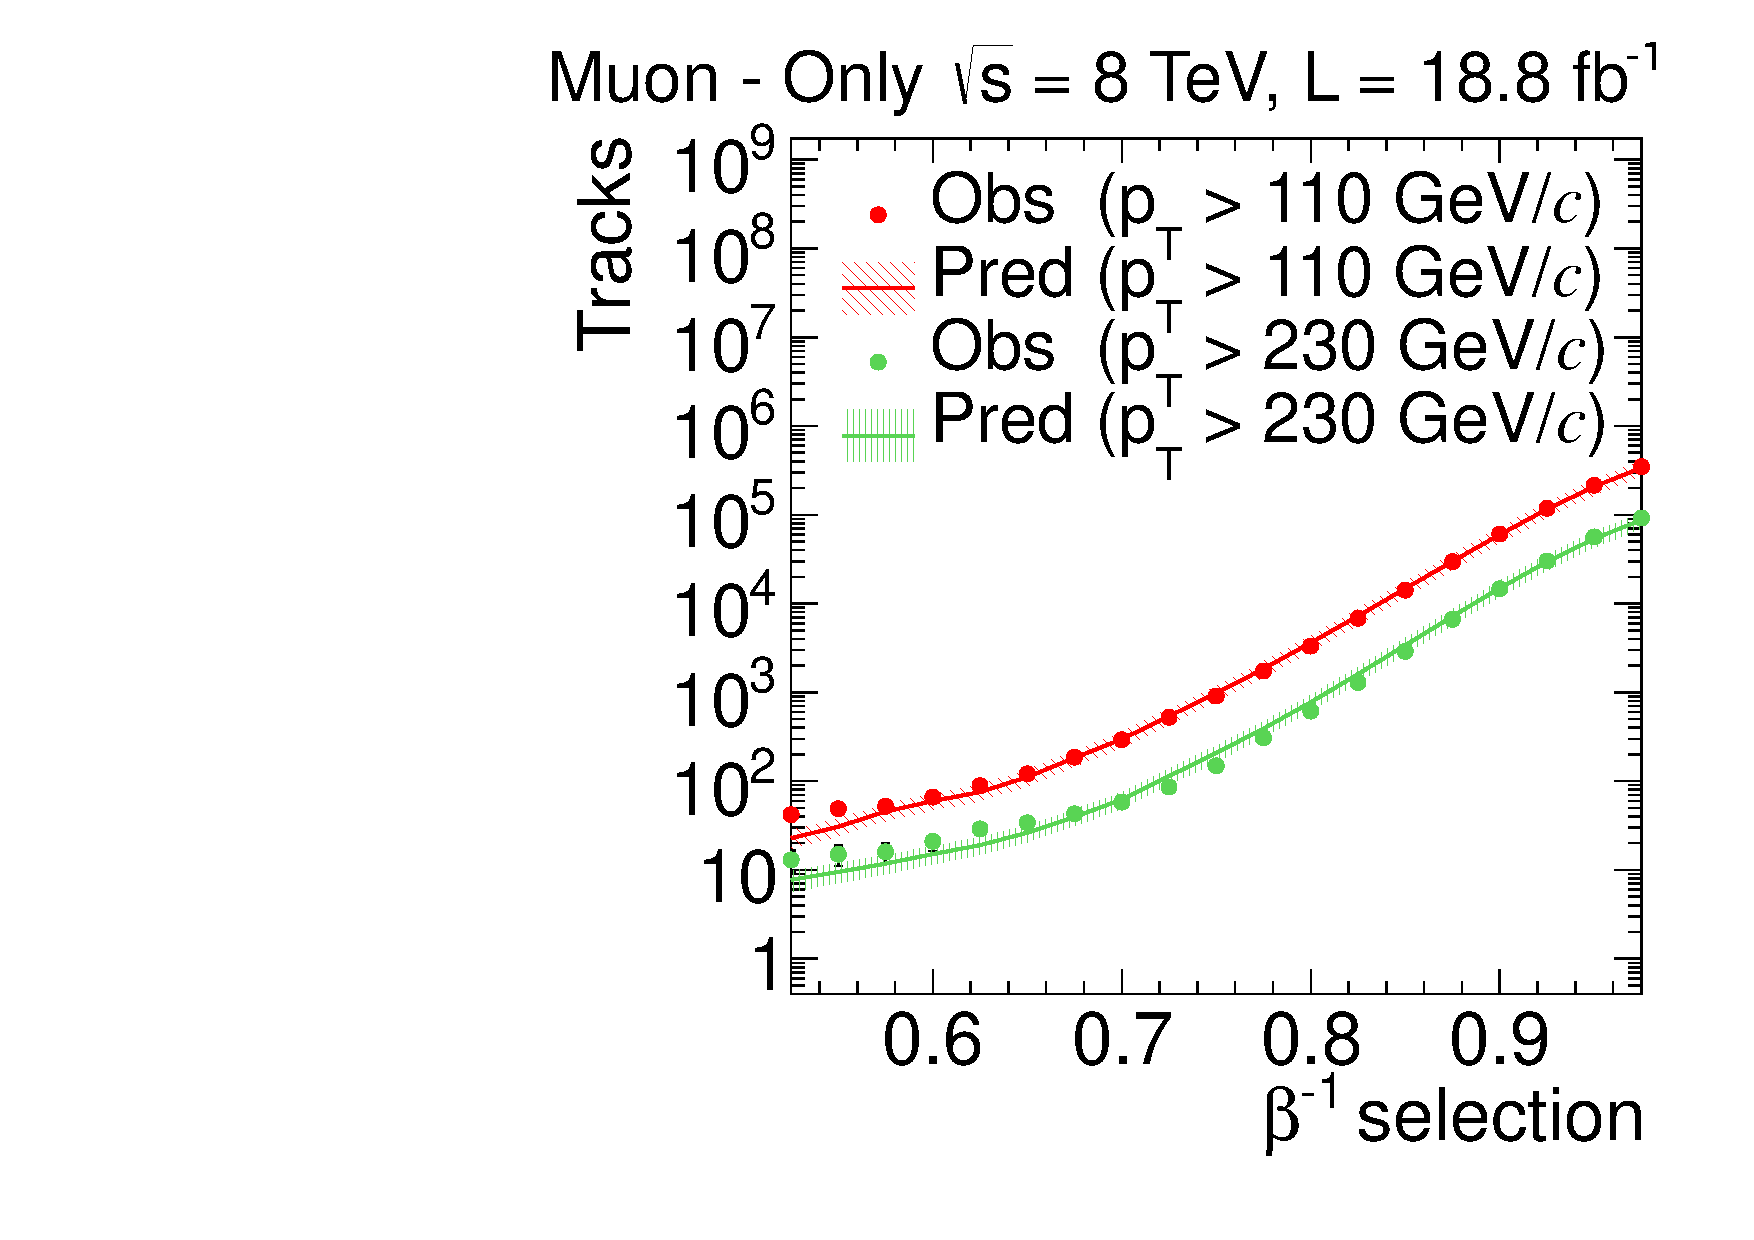
\includegraphics[clip=false, trim=0.0cm 0cm 0.0cm 0cm, width=0.48\textwidth]{figures/muonly/Prediction_Data8TeV_NPredVsNObs_Flip}
  \caption[Number of predicted and observed tracks in the \invbeta\ $<$ 1 region in the \muononly\ analysis]
{Number of predicted and observed tracks passing thresholds on \pt\ and \invbeta. The tracks are required to be above the \pt\ threshold and below the \invbeta\ threshold.
Two representative $p_T$ thresholds are shown. Threshold for \invbeta\ set by x-axis.
Figure is cumulative, as tracks passing the selection with tight thresholds will also pass for loose thresholds.}
    \label{fig:PredFlipPt230}
\end{figure}

To determine the systematic uncertainty on the predicted collision background, the \invbeta\ $<$ 1 region is used once again. The predicted number of tracks
in the signal region D can be predicted by three different formulae: the main one of $B \times C/A$, as well as 
$B \times C^{\prime}/A^{\prime}$ and $B \times D^{\prime}/B^{\prime}$. The $B$ region contains tracks with \invbeta\ above the final selection threshold and
\pt\ below its threshold. The ratios $C/A$, $C^{\prime}/A^{\prime}$, and $D^{\prime}/B^{\prime}$ give the fraction of tracks to be above the threshold on \pt\
in the region with \invbeta\ between one and the final threshold; the region with \invbeta\ between a value less than one, for example 0.8, and one;
and the region with \invbeta\ below
the same less than one value, respectively. Thus the different predictions can be used to evaluate how the fraction of background tracks to pass the \pt\ threshold depends on
their \invbeta.
%The first of the additional predictions would be sensitive to any shift in the \invbeta\ distribution due to the $p_T$ requirement while the second would be
%sensitive to any effect on the resolution due to the $p_T$ requirement. 
Figure~\ref{fig:MuOnlycorrelation} shows the number of predicted tracks from the three predictions for different \invbeta\ and $p_T$ thresholds.

\begin{figure}
\begin{center}
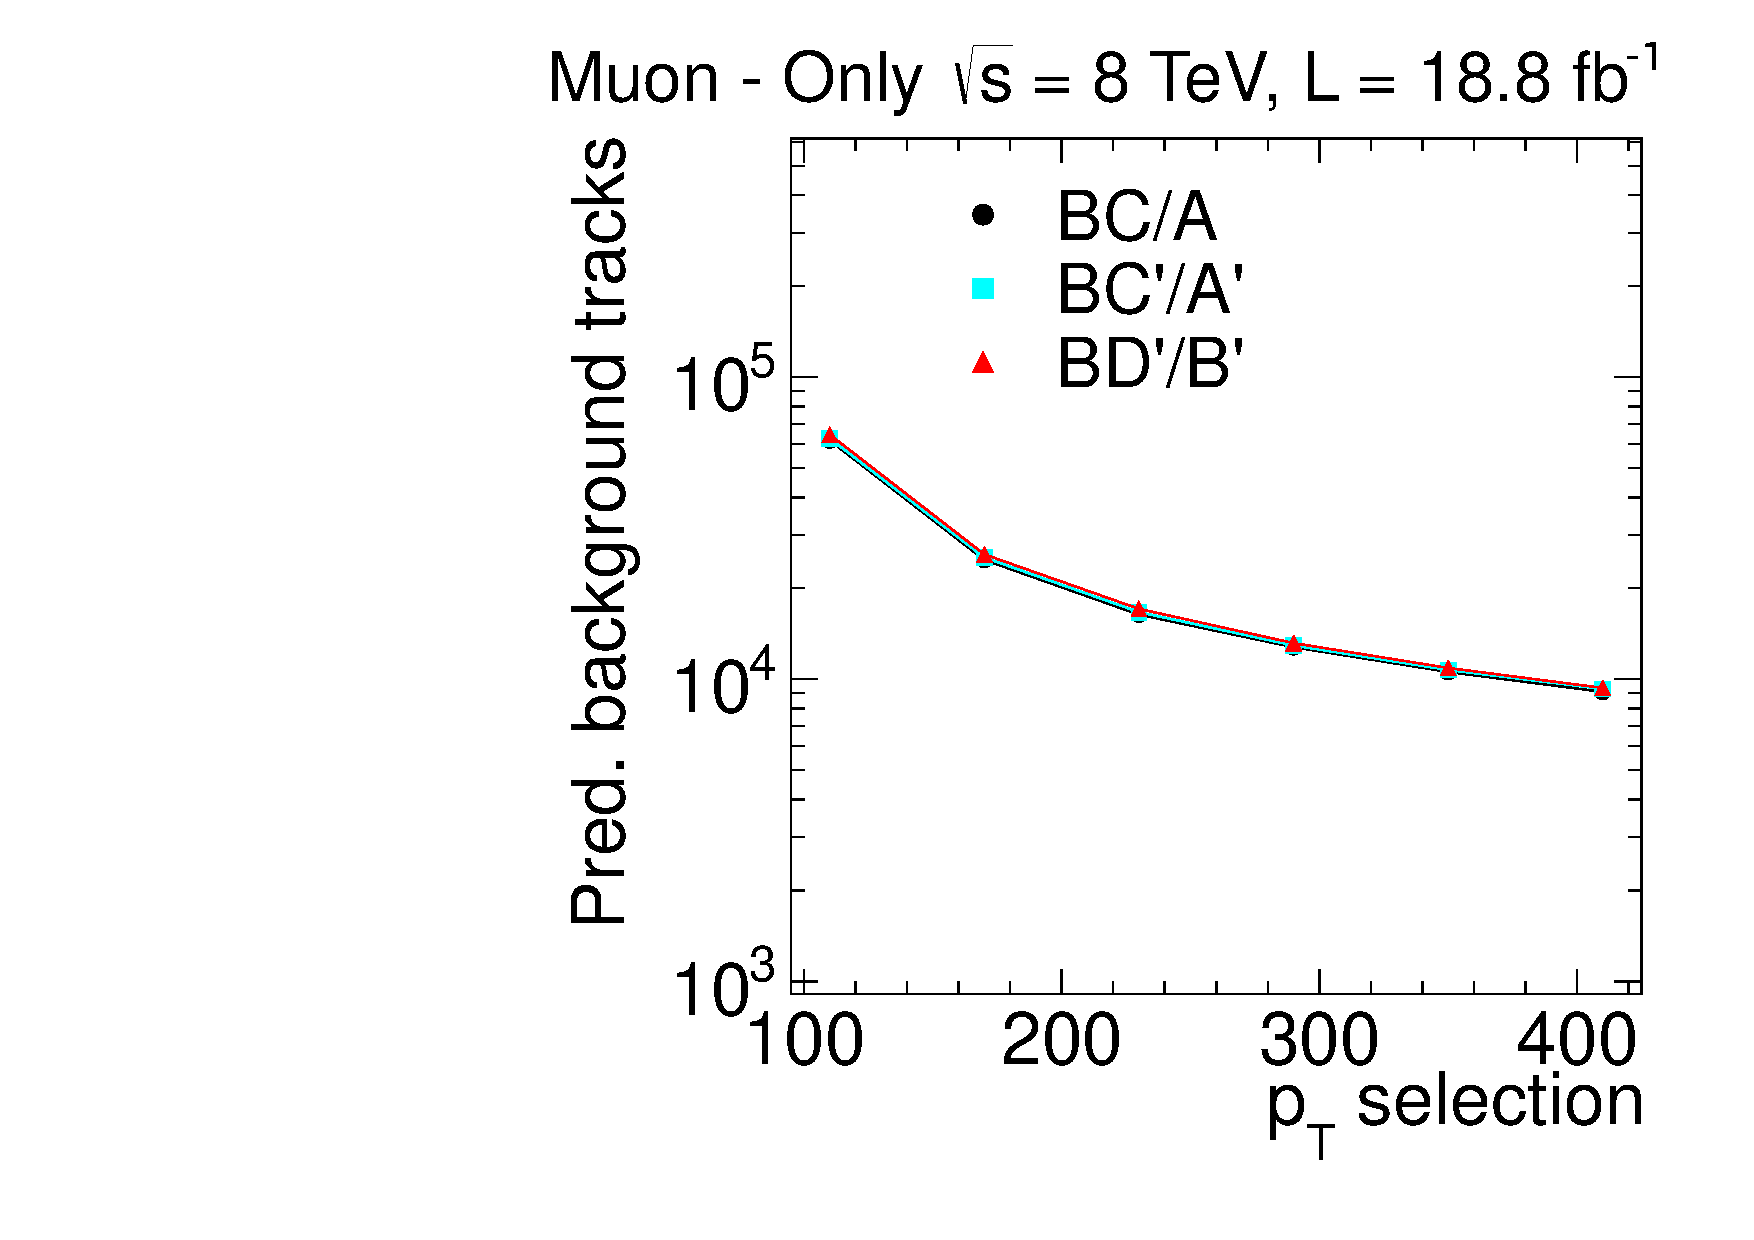
\includegraphics[clip=false, trim=0.0cm 0cm 0.0cm 0cm, width=0.48\textwidth]{figures/muonly/Data8TeVCollisionPrediction_TOF110}
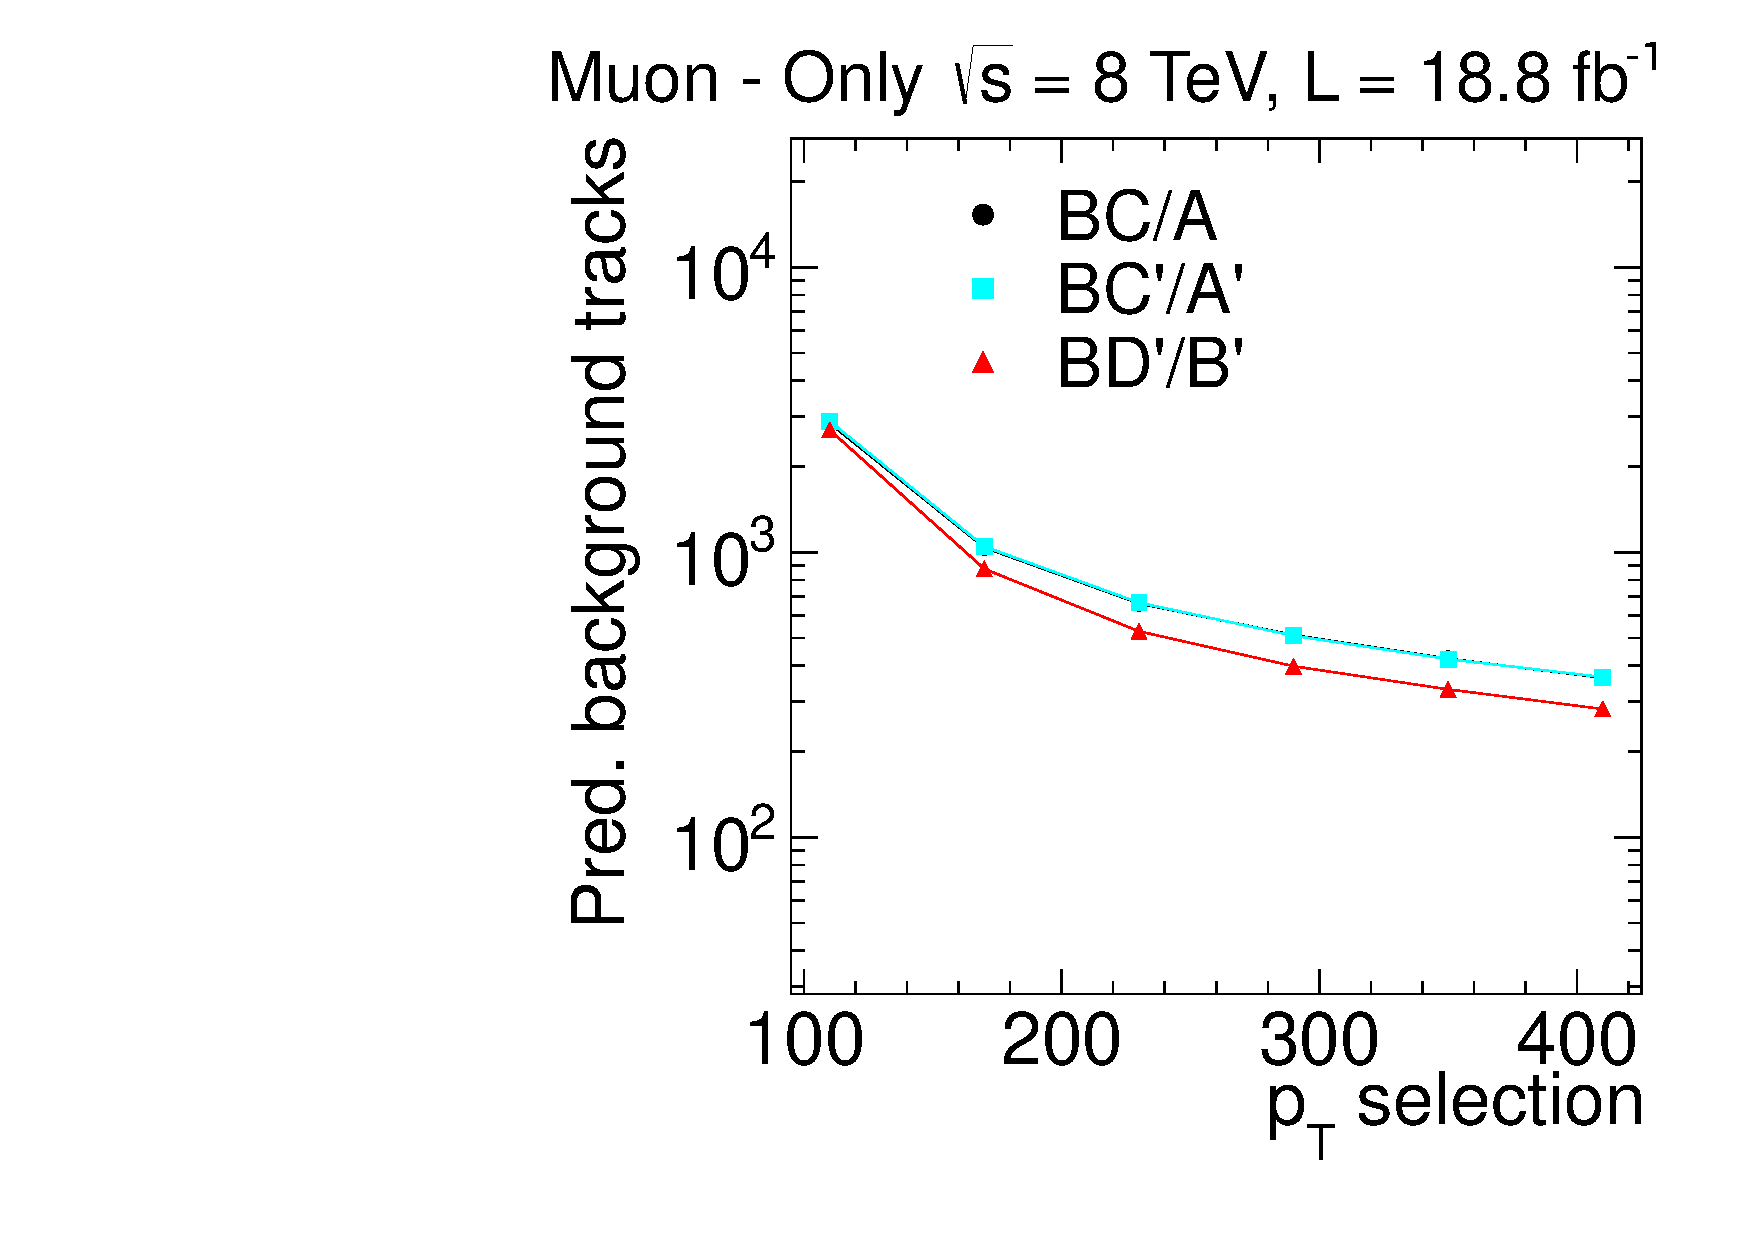
\includegraphics[clip=false, trim=0.0cm 0cm 0.0cm 0cm, width=0.48\textwidth]{figures/muonly/Data8TeVCollisionPrediction_TOF120}
\caption[Distributions of the number of predicted tracks with different prediction formulae for different sets of thresholds in the \muononly\ analysis.]
{Distributions of the number of predicted tracks and their statistical uncertainty with different prediction formulae for different sets of thresholds.
The $p_{T}$ threshold is defined by the x-axis.
Figures are cumulative, as tracks passing the selection with tight thresholds will also pass for loose thresholds.
Left: $1/\beta>1.1$ ($<0.9$ for low $1/\beta$ regions). Right: $1/\beta>1.2$ ($<0.8$ for low $1/\beta$ regions).}
\label{fig:MuOnlycorrelation}
\end{center}
\end{figure}

The systematic uncertainty is extracted from the three predictions
through Eq.~\ref{eq:variance} with N=3.
Fig.~\ref{fig:MuOnlyUnc} shows the variation of
$S_{syst+stat}/\langle x \rangle $, $S_{stat}/ \langle x \rangle $ and the extracted $S_{syst}/ \langle x \rangle $
as a function of the $p_T$ threshold. The statistical uncertainty due to the number of tracks in the $B$ group is not subtracted as it is completely correlated
between the three predictions. From the last plot
the systematic uncertainty on the expected background in the signal
region is placed at 20\%.

\begin{figure}
\begin{center}
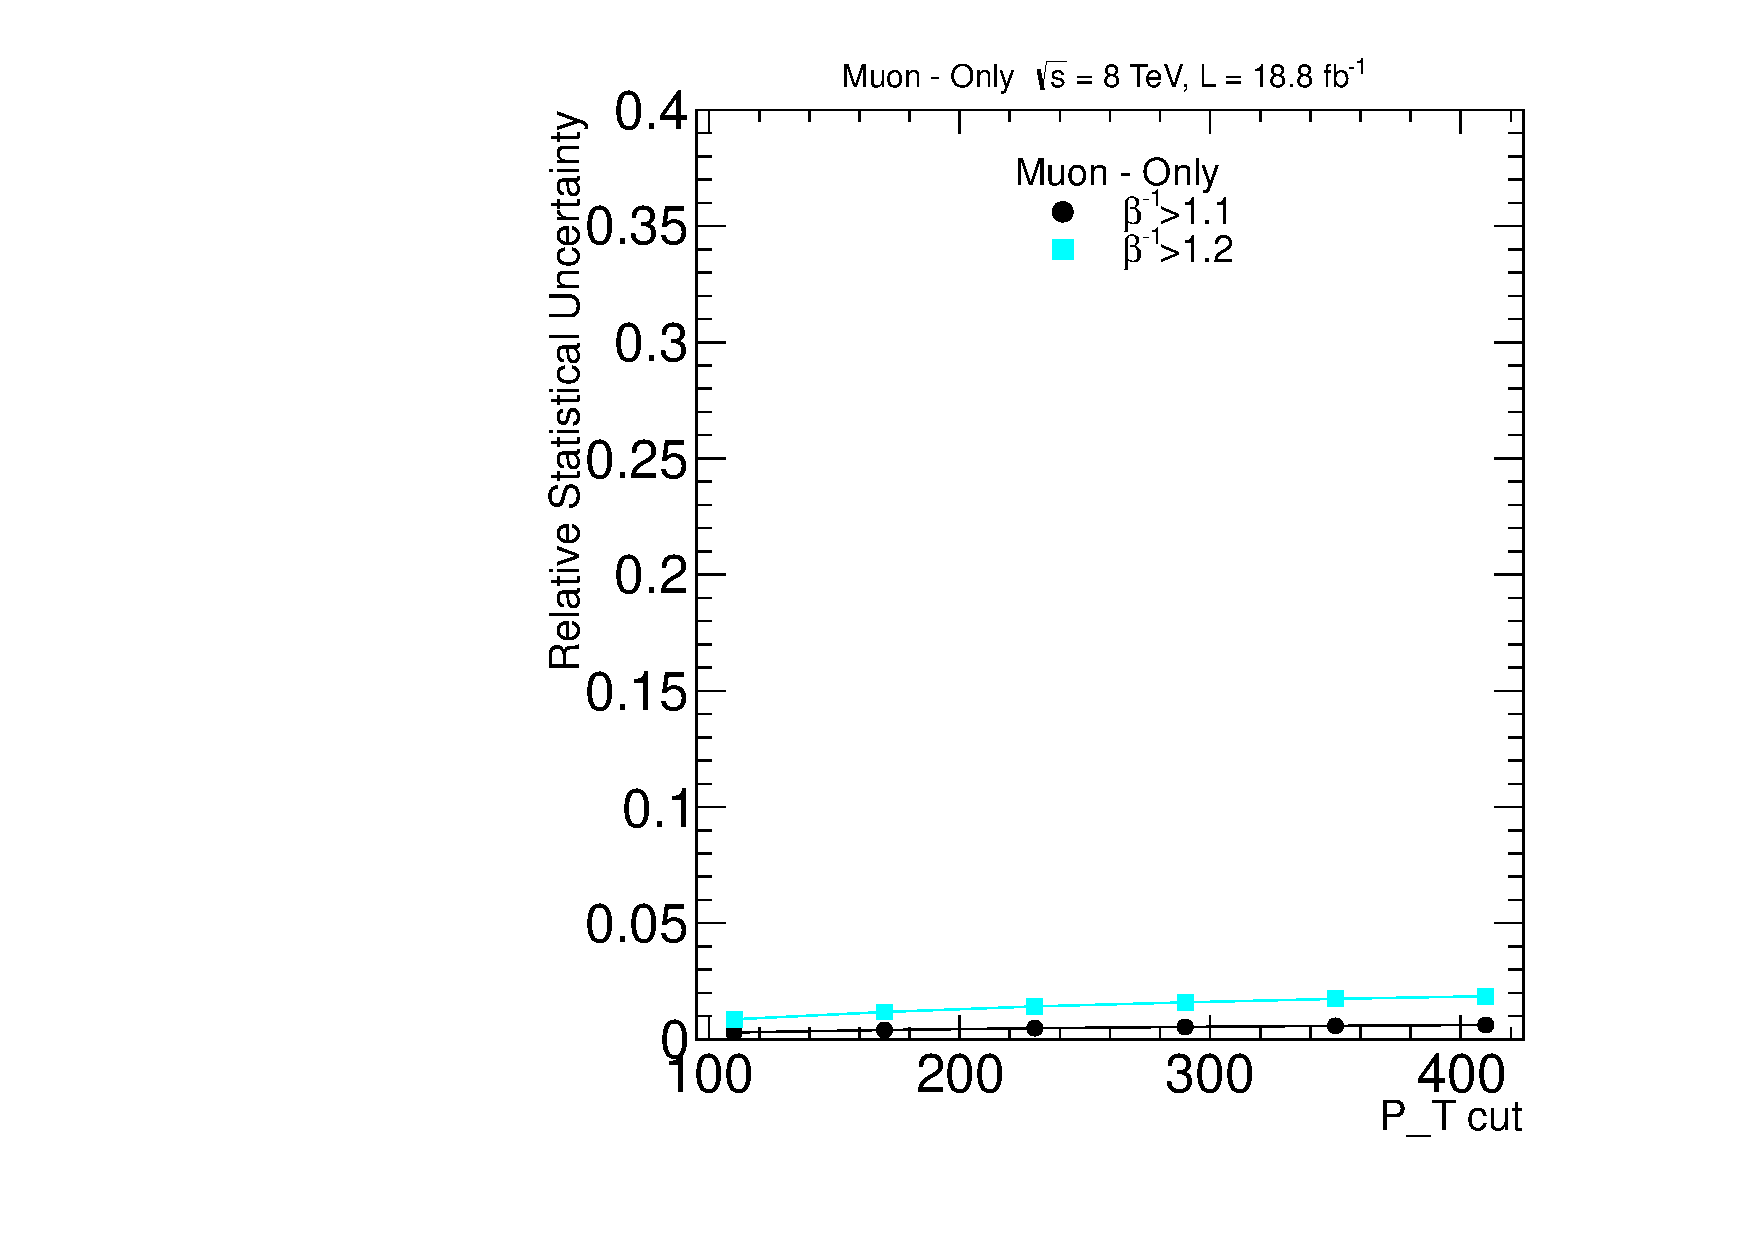
\includegraphics[clip=false, trim=0.0cm 0cm 0.0cm 0cm, width=0.48\textwidth]{figures/muonly/Data8TeVCollisionStat}
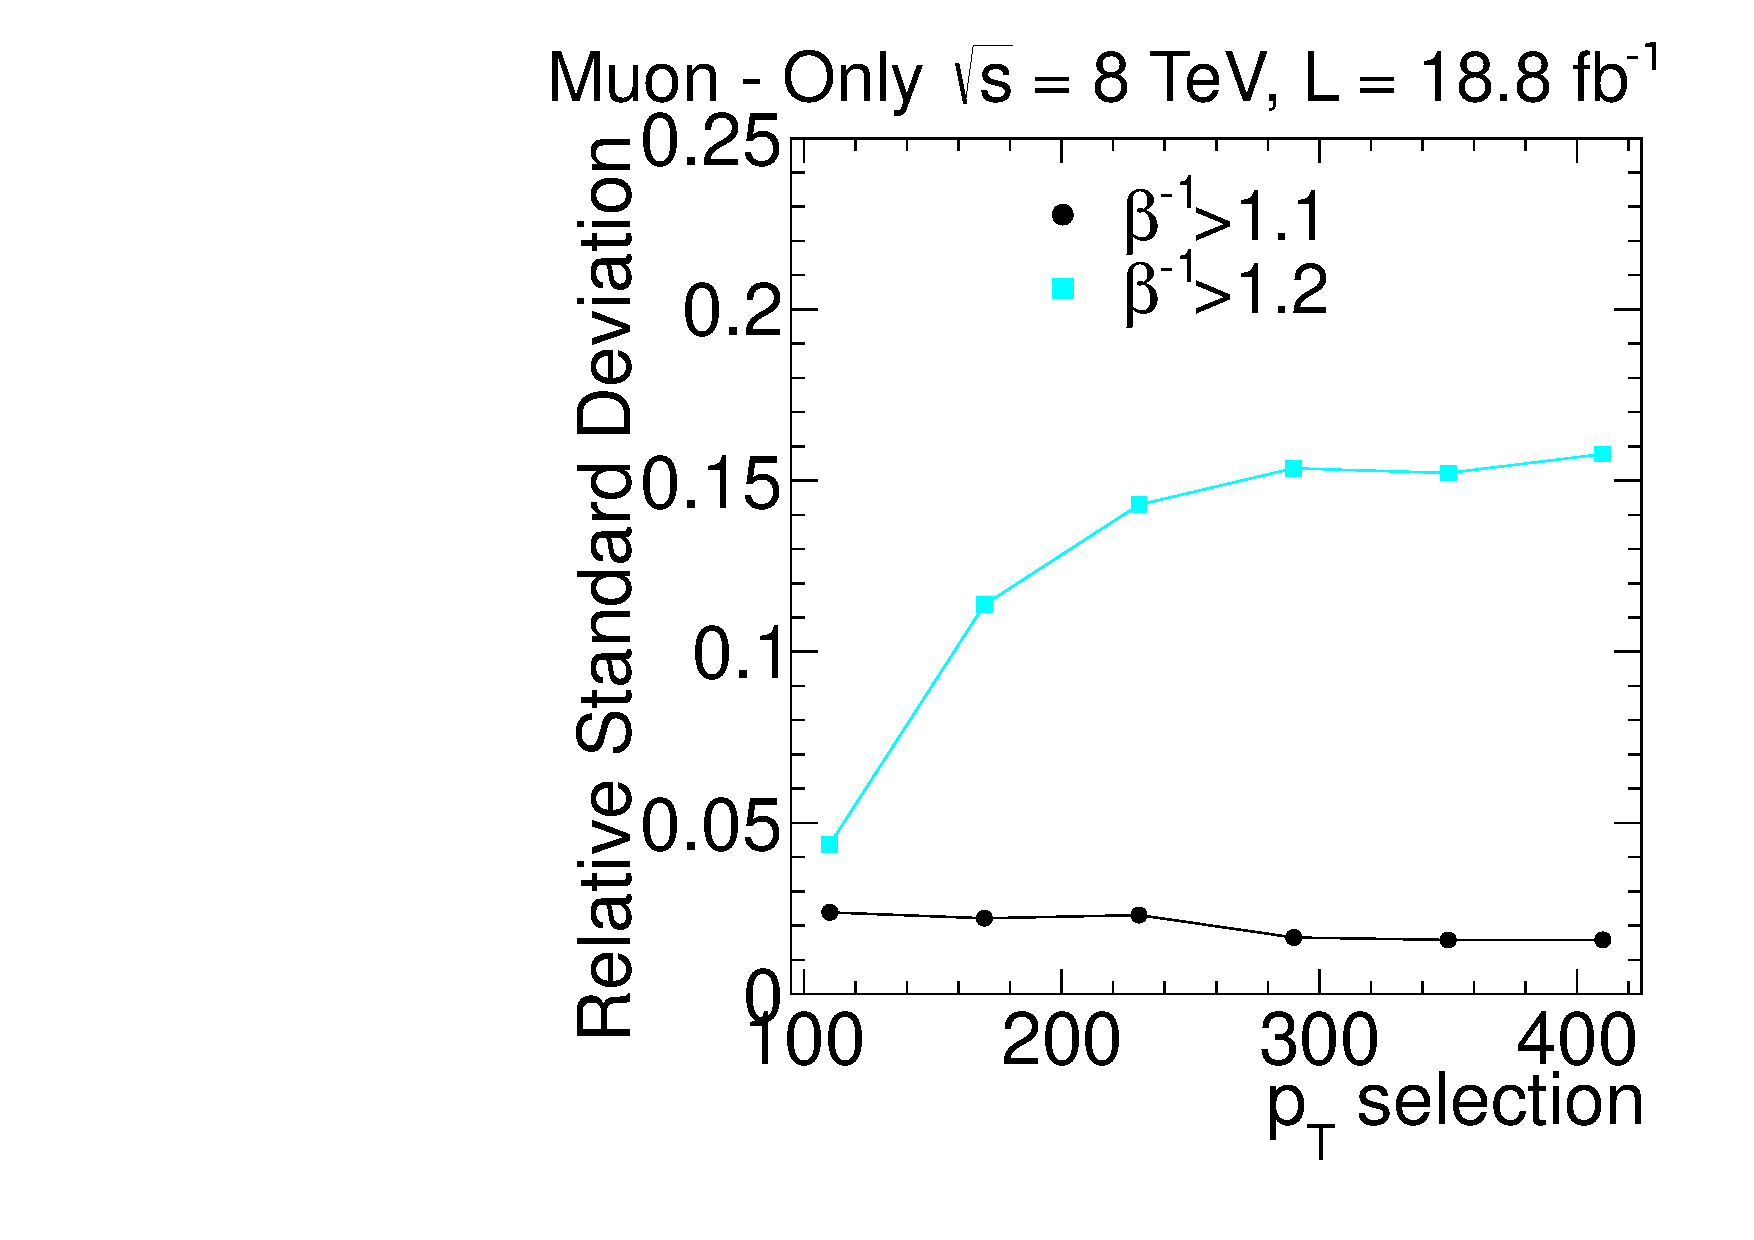
\includegraphics[clip=false, trim=0.0cm 0cm 0.0cm 0cm, width=0.48\textwidth]{figures/muonly/Data8TeVCollisionStatSyst} \\
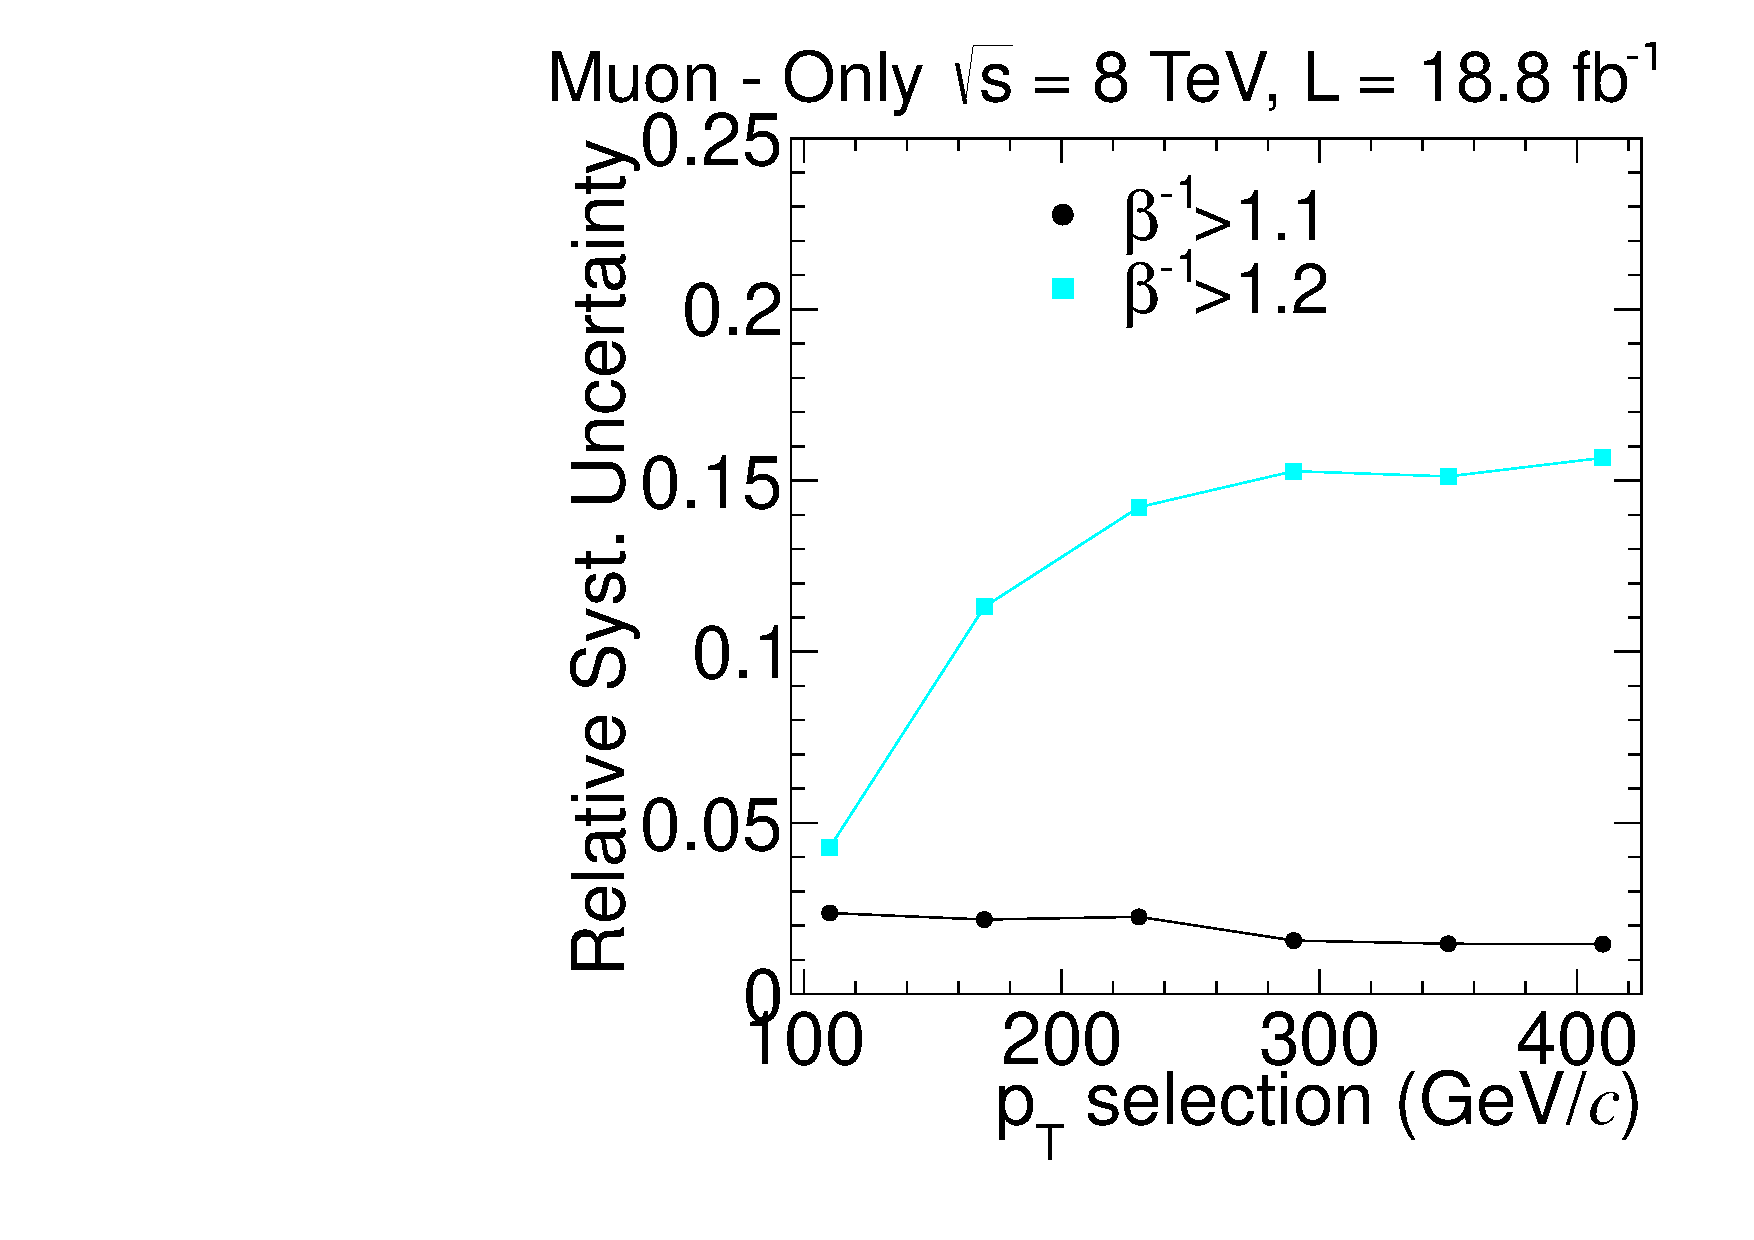
\includegraphics[clip=false, trim=0.0cm 0cm 0.0cm 0cm, width=0.48\textwidth]{figures/muonly/Data8TeVCollisionSyst}
\caption[Statistical and systematic uncertainties in the background prediction for different sets of thresholds in the \muononly\ analysis.]
{Relative uncertainty on the collision-muon background prediction in the \muononly\ analysis.
Two different \invbeta\ thresholds are plotted. Threshold on \pt\ set by the $x$-axis.
Plots show $S^{syst+stat}_{3}/\langle x \rangle$ (top left), $S^{stat}_{3}\langle x \rangle$ (top right), and $S^{syst}_{3}\langle x \rangle$ (bottom)
where $\langle x \rangle$ is the average predicted background.
The uncertainty variables are defined in Equation~\ref{eq:variance}.
%Ratio of the square root of the quadratic
%mean of the statistical (stat.) uncertainties of the three possible background
%estimations to the mean of these estimations vs
%the $p_T$ selection. Top right: Ratio of the standard deviation to the mean of the three
%background estimations vs the $p_T$ selection. Bottom: Ratio of the
%square root of the difference between the variance and the quadratic
%mean of the statistical uncertainties of the three possible background
%estimations and the mean vs the $p_T$ selection, taken as an estimate of the relative systematic (syst) uncertainty.
}
\label{fig:MuOnlyUnc}
\end{center}
\end{figure}

The systematic uncertainty on the cosmic-ray-muon background is determined by
modifying the $d_z$ range used to define the control sample.  Predictions
can also be made from tracks with $30 < |d_z| < 50$~cm, $50 < |d_z| < 70$~cm, and
120~cm~$< |d_z|$.  Table~\ref{tab:CosmicPred} shows the number of predicted cosmic-ray muons
for each $|d_z|$ region using the final selection defined in Section~\ref{sec:Optim}.
The statistical uncertainty from the number of tracks in the signal region in the
pure cosmic-ray muon sample is not included in the uncertainties listed as it is correlated
between the three predictions.
Equation~\ref{eq:variance} with N=4 is used to calculate the systematic uncertainty.
The observed $S^{stat}$ is larged than the observed $S^{syst+stat}$, meaning the agreement between the measurements is better than
would be expected based on their statistical uncertainties alone.
This indicates that the uncertainty on the cosmic-ray muon background prediction is dominated by the statistical uncertainty, however, an 80\% relative systematic uncertainty 
is placed on the prediction to be conservative.

\begin{table}
 \begin{center}
  \caption{Predicted numbers of cosmic-ray muon tracks for the \muononly\ analysis for various choices of control region.}
     \label{tab:CosmicPred}
  \begin{tabular}{|l|c|c|} \hline
   $|d_z|$ Region            & Prediction  \\ \hline
   $30 < |dz| < 50$~cm  & 3.1 $\pm$ 0.5   \\ \hline
   $50 < |dz| < 70$~cm  & 2.6 $\pm$ 0.7   \\ \hline
   $70 < |dz| < 120$~cm & 3.2 $\pm$ 1.0   \\ \hline
   120~cm~$< |dz|$      & 3.8 $\pm$ 0.7   \\ \hline
  \end{tabular}
 \end{center}
\end{table}

\subsection{Prediction for \tktof\ analysis}

The \tktof\ analysis uses three selection variables, $p_T$, \invbeta, and \ias. With three selection variables an extended three dimensional version of the 
$ABCD$ method is used to predict the collision-muon background. An additional requirement on the reconstructed mass of the track
is also applied and the prediction of the background mass spectrum is described below. 
For each signal point, the reconstructed mass of tracks must be above the average reconstructed mass of the signal minus two sigma of the mass
distribution (both determined from MC) and below 2 TeV/$c^2$.
As discussed above, the cosmic-ray-muon background is negligible
for the \tktof\ analysis. 

To test if the selection variables are uncorrelated, the distribution of one of the variables is plotted for numerous ranges of one of the other variables.
If the variables are uncorrelated then the distributions should all be the same. 
The distributions are shown in Fig.~\ref{fig:correlation} and the variables are found to be sufficiently uncorrelated.

\begin{figure}%[tbhp!]
\begin{center}
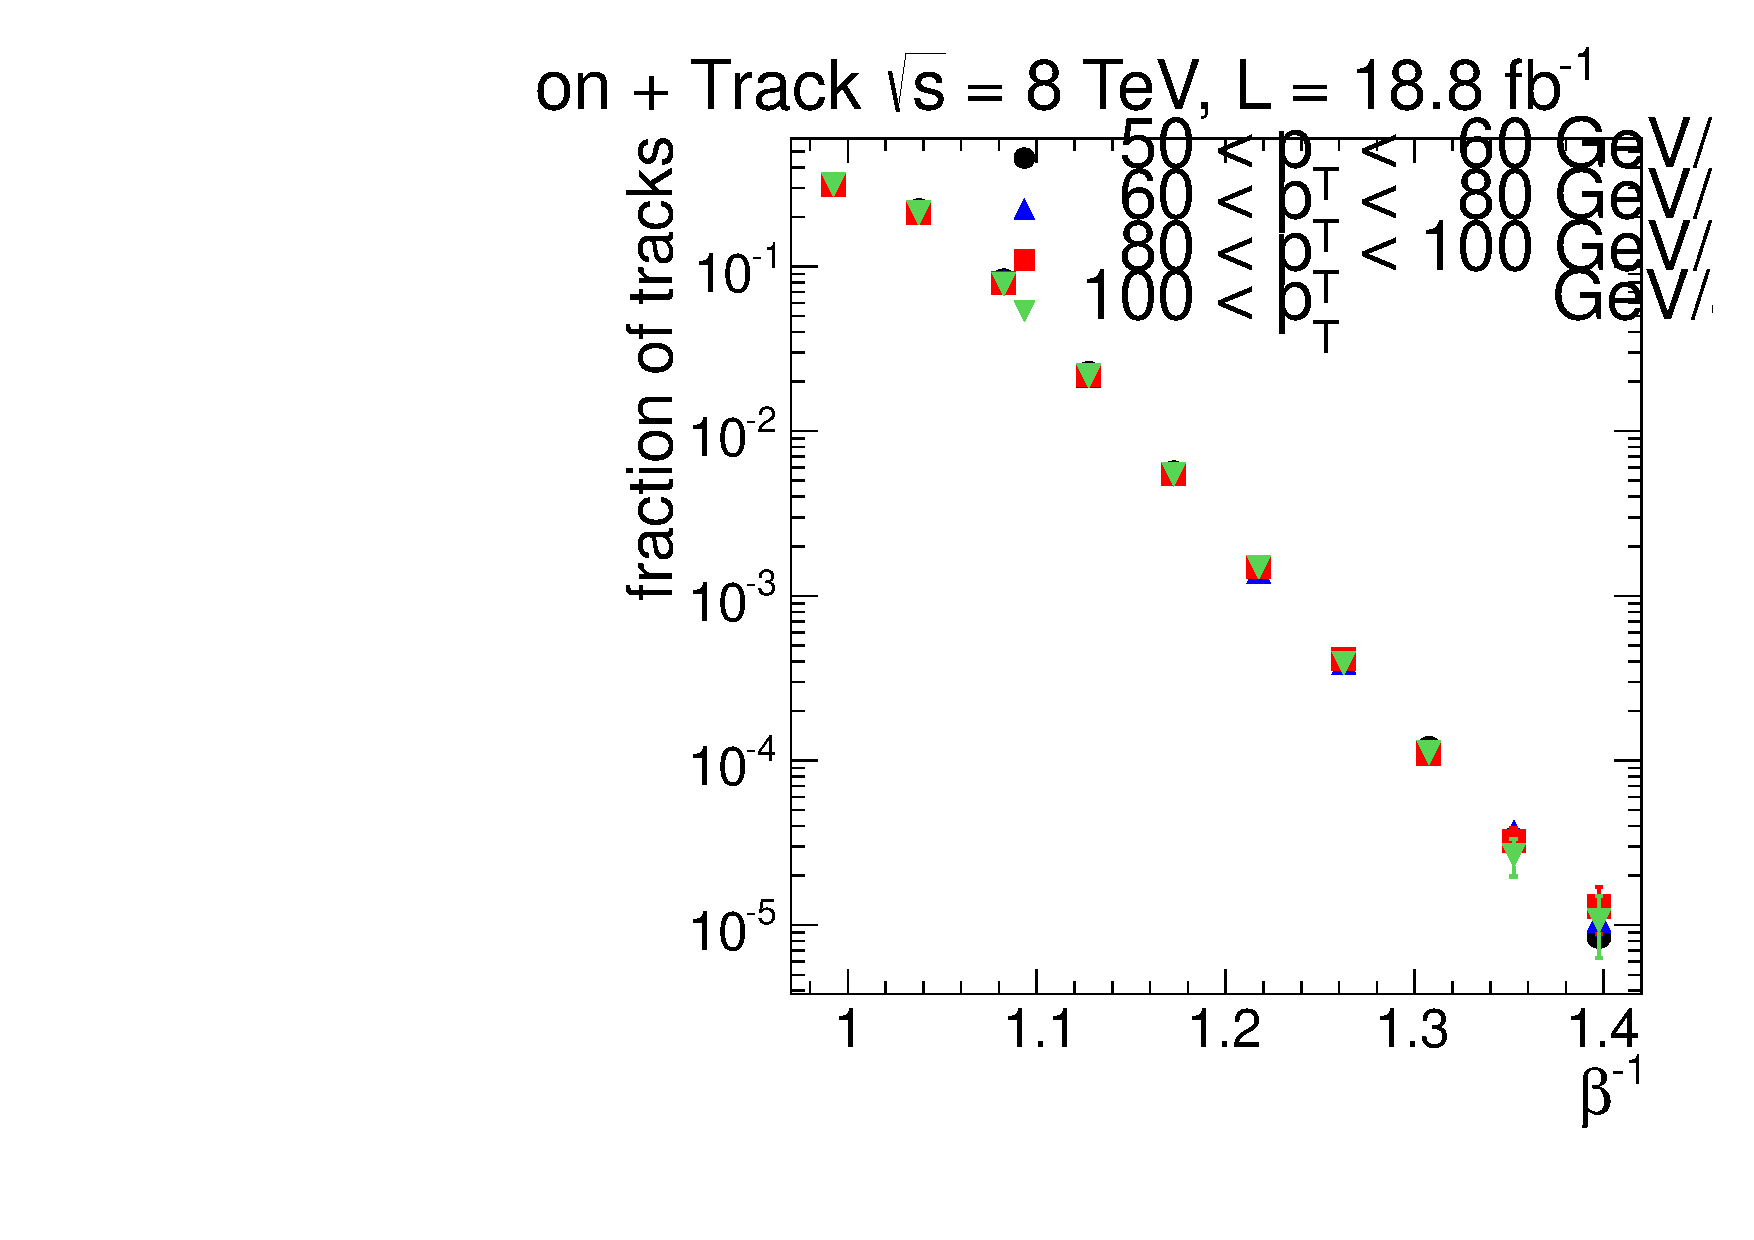
\includegraphics[clip=false, trim=0.0cm 0cm 0.0cm 0cm, width=0.48\textwidth]{figures/tkmu/Control_Data8TeV_Pt_TOFSpectrum}
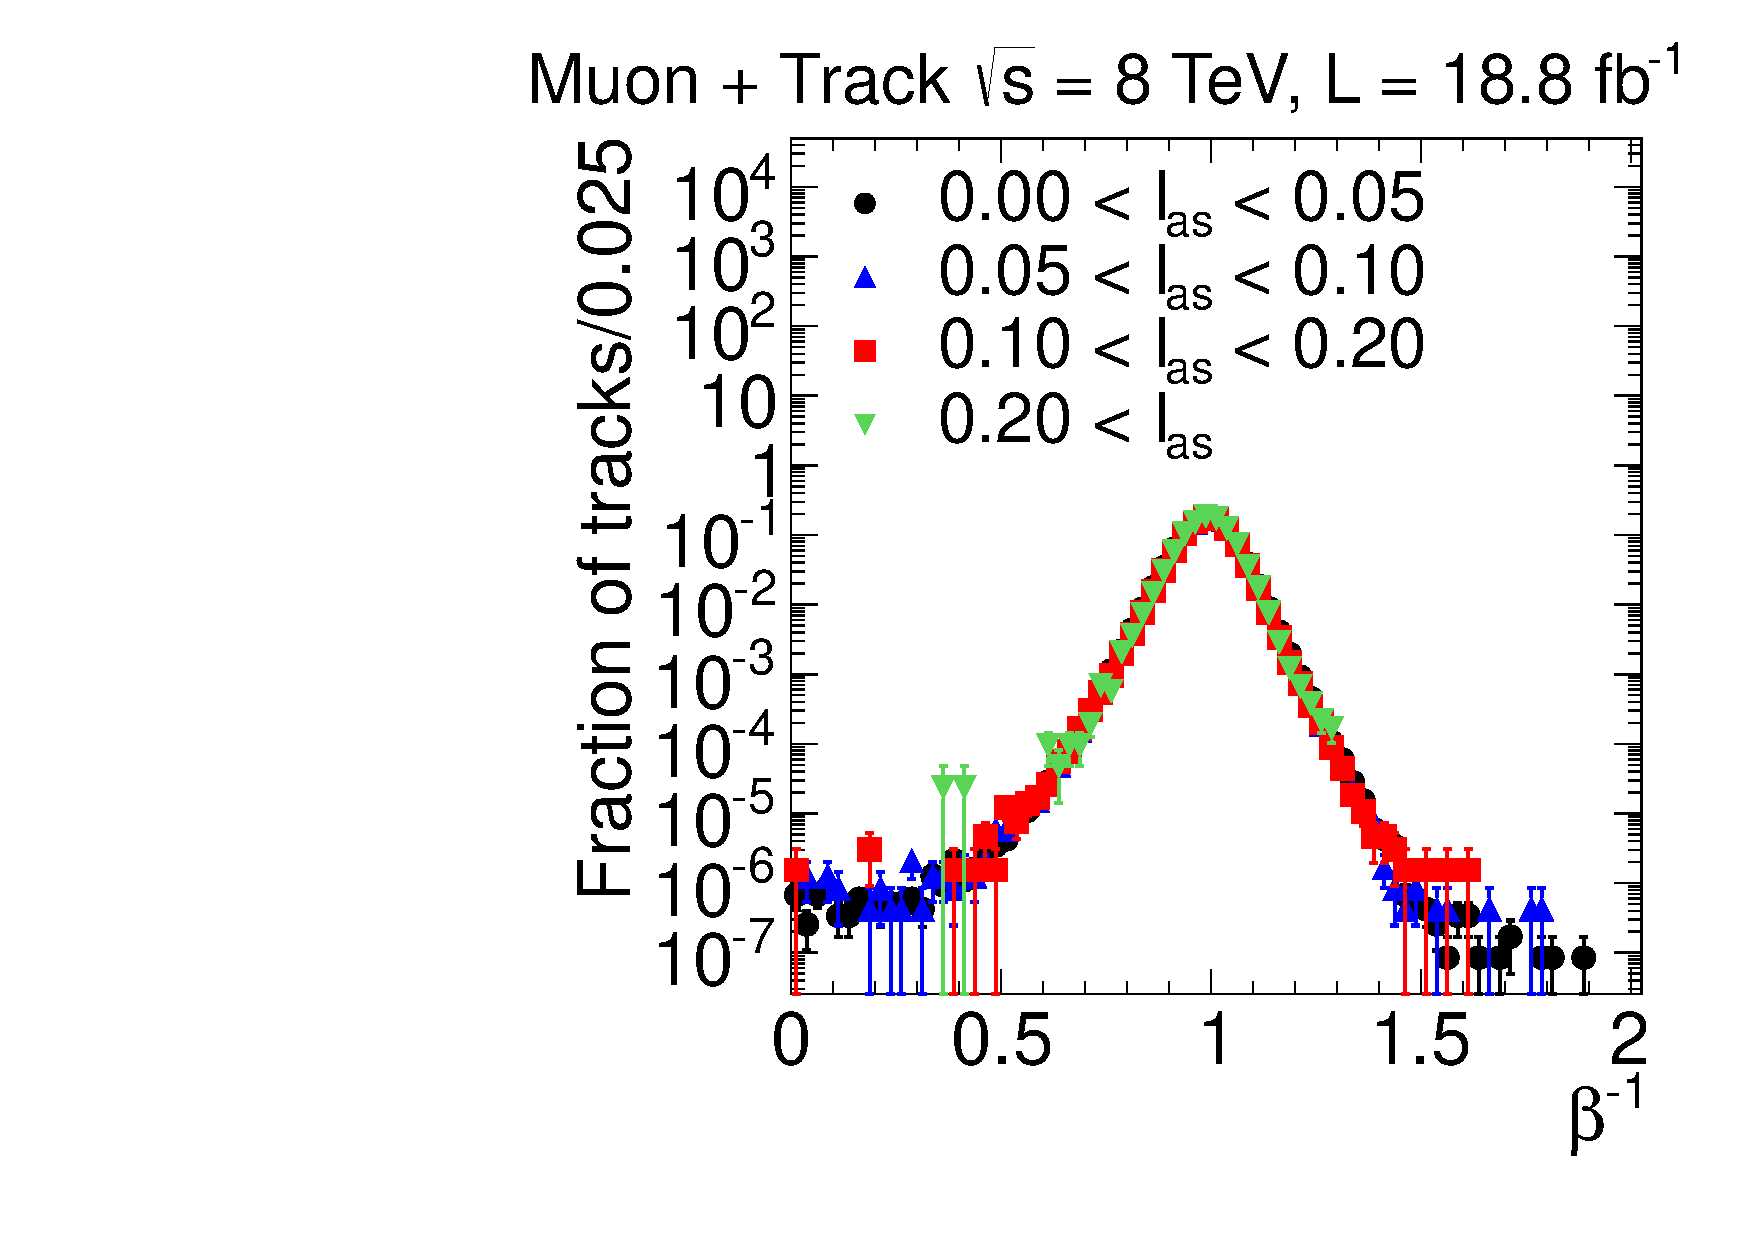
\includegraphics[clip=false, trim=0.0cm 0cm 0.0cm 0cm, width=0.48\textwidth]{figures/tkmu/Control_Data8TeV_Is_TOFSpectrumLog}
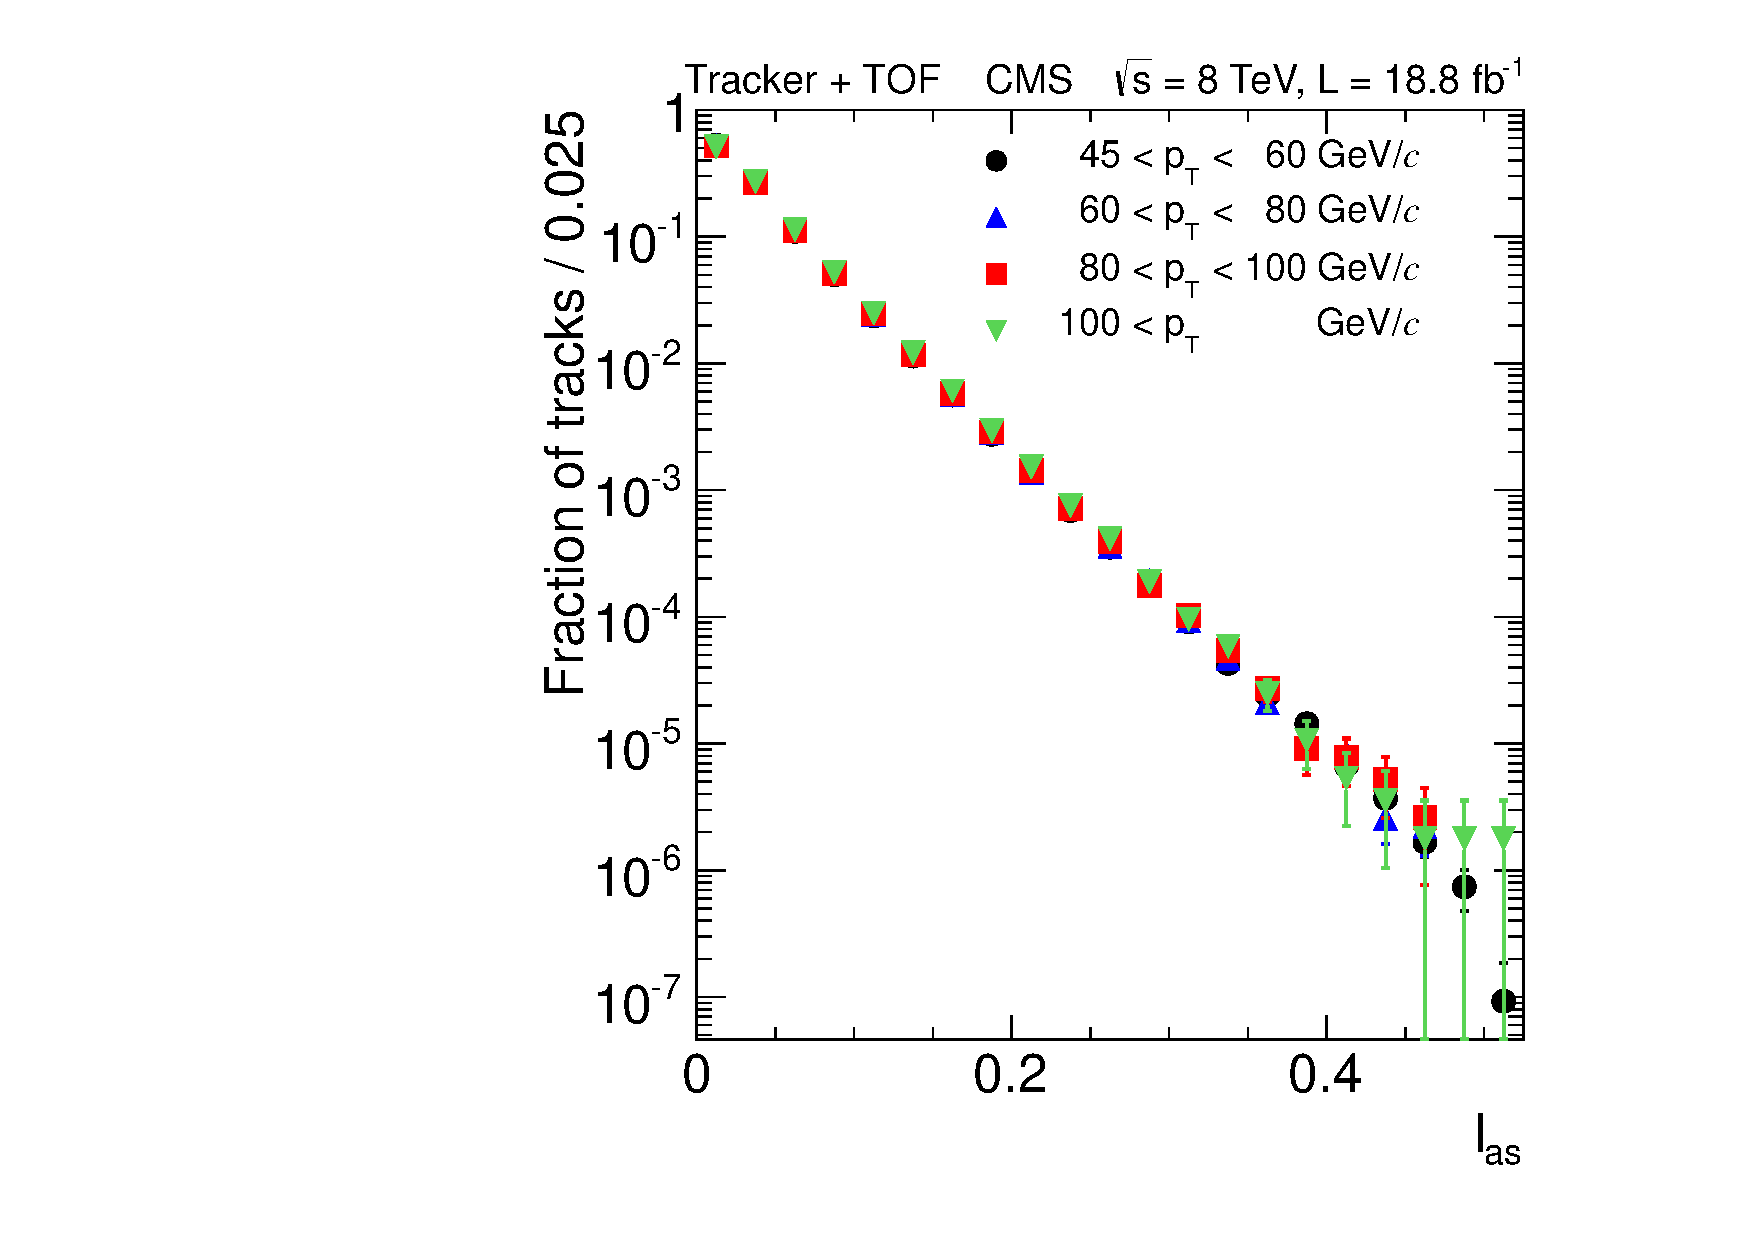
\includegraphics[clip=false, trim=0.0cm 0cm 0.0cm 0cm, width=0.48\textwidth]{figures/tkmu/Control_Data8TeV_Pt_IsSpectrum}
\caption[Distribution of selection variables in the \tktof\ analysis for different ranges of the other variables]
{Top row: Measured \invbeta\ distributions for several momentum ranges (left)
and \ias\ ranges (right). Bottom row:  Measured \ias\ distributions for several momentum  ranges.
}
\label{fig:correlation}
\end{center}
\end{figure}

%Four new groups are defined, $E$, $F$, $G$, and $H$. The D region still represents
%the signal region where the track passes the thresholds on all three selection variables. The $B$, $C$, and $H$ regions pass two of the thresholds and fail \invbeta,
%$p_T$, and $\dedx,$ respectively. The $A$, $F$, and $G$ groups contain tracks passing only the \dedx, \invbeta, and $p_T$ thresholds, respectively.
Since the \tktof\ analysis employs three selection variables it uses all eight bins defined in Table~\ref{tab:BinNames}.
With eight bins, the number of predicted tracks in the signal region, $D$, can be found via seven different equations utilizing the various bins.
The predictions can be divided into three groups characterized by the amount of statistical uncertainty they have.
The prediction $A\times F\times G/E^2$ has the smallest statistical uncertainty as it uses only the bins with at most one of the selection thresholds being passed.
For this reason it is selected to determine the background estimate in the search.
The predictions $A\times H / E$, $G\times B / E$, and $F\times C / E$ all use one of the bins where two of the thresholds have been passed.
This results in them having a slightly larger statistical uncertainty (approximately a factor of 2--5 depending on the thresholds used).
These predictions are used to determine the systematic uncertainty on the background prediction.
The predictions $H\times C / G$, $C\times B / A$, and $H\times B / F$ include two of the bins that have tracks passing two of the thresholds giving it a much larger
statistical uncertainty (factor of ten larger). These predictions are not used in the analysis.

As with the \muononly\ analysis the background prediction is additionally checked with tracks in the \invbeta\ less than one region. Again the predicted number of tracks in
$D^{\prime}$ is estimated following the same procedure as for the signal region except changing the \invbeta\ requirement to be lower than some threshold,
i.e. $D^{\prime} = A^{\prime}\times F^{\prime}\times G^{\prime} / E^{\prime 2}$.
Figure~\ref{fig:PredFlipTkTOF} shows the predicted and observed number of tracks in the $D^{\prime}$ region for representative loose and tight thresholds. 
Good agreement is seen even with a tight selection.

\begin{figure}
\begin{center}
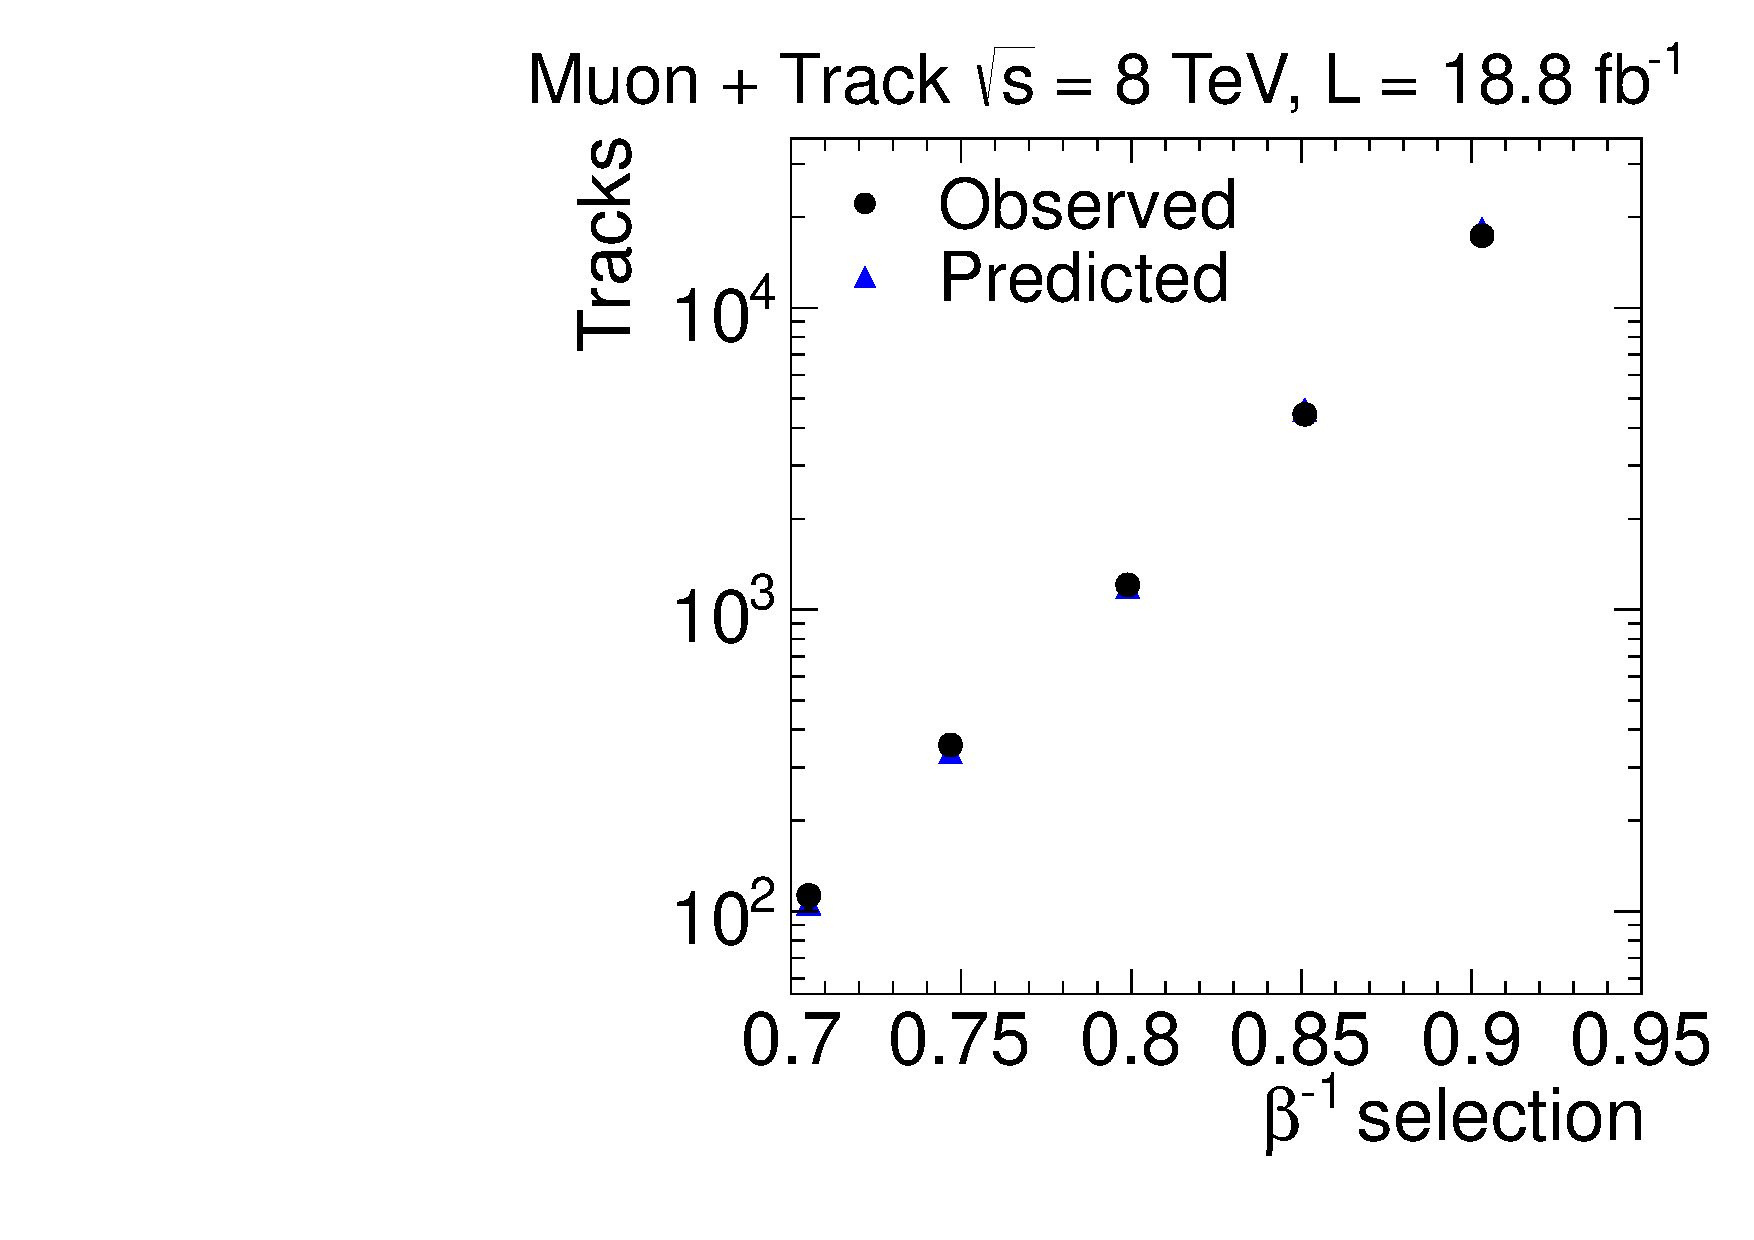
\includegraphics[clip=false, trim=0.0cm 0cm 0.0cm 0cm, width=0.48\textwidth]{figures/tkmu/Pred_Flip_I010_Pt55_Data8TeV}
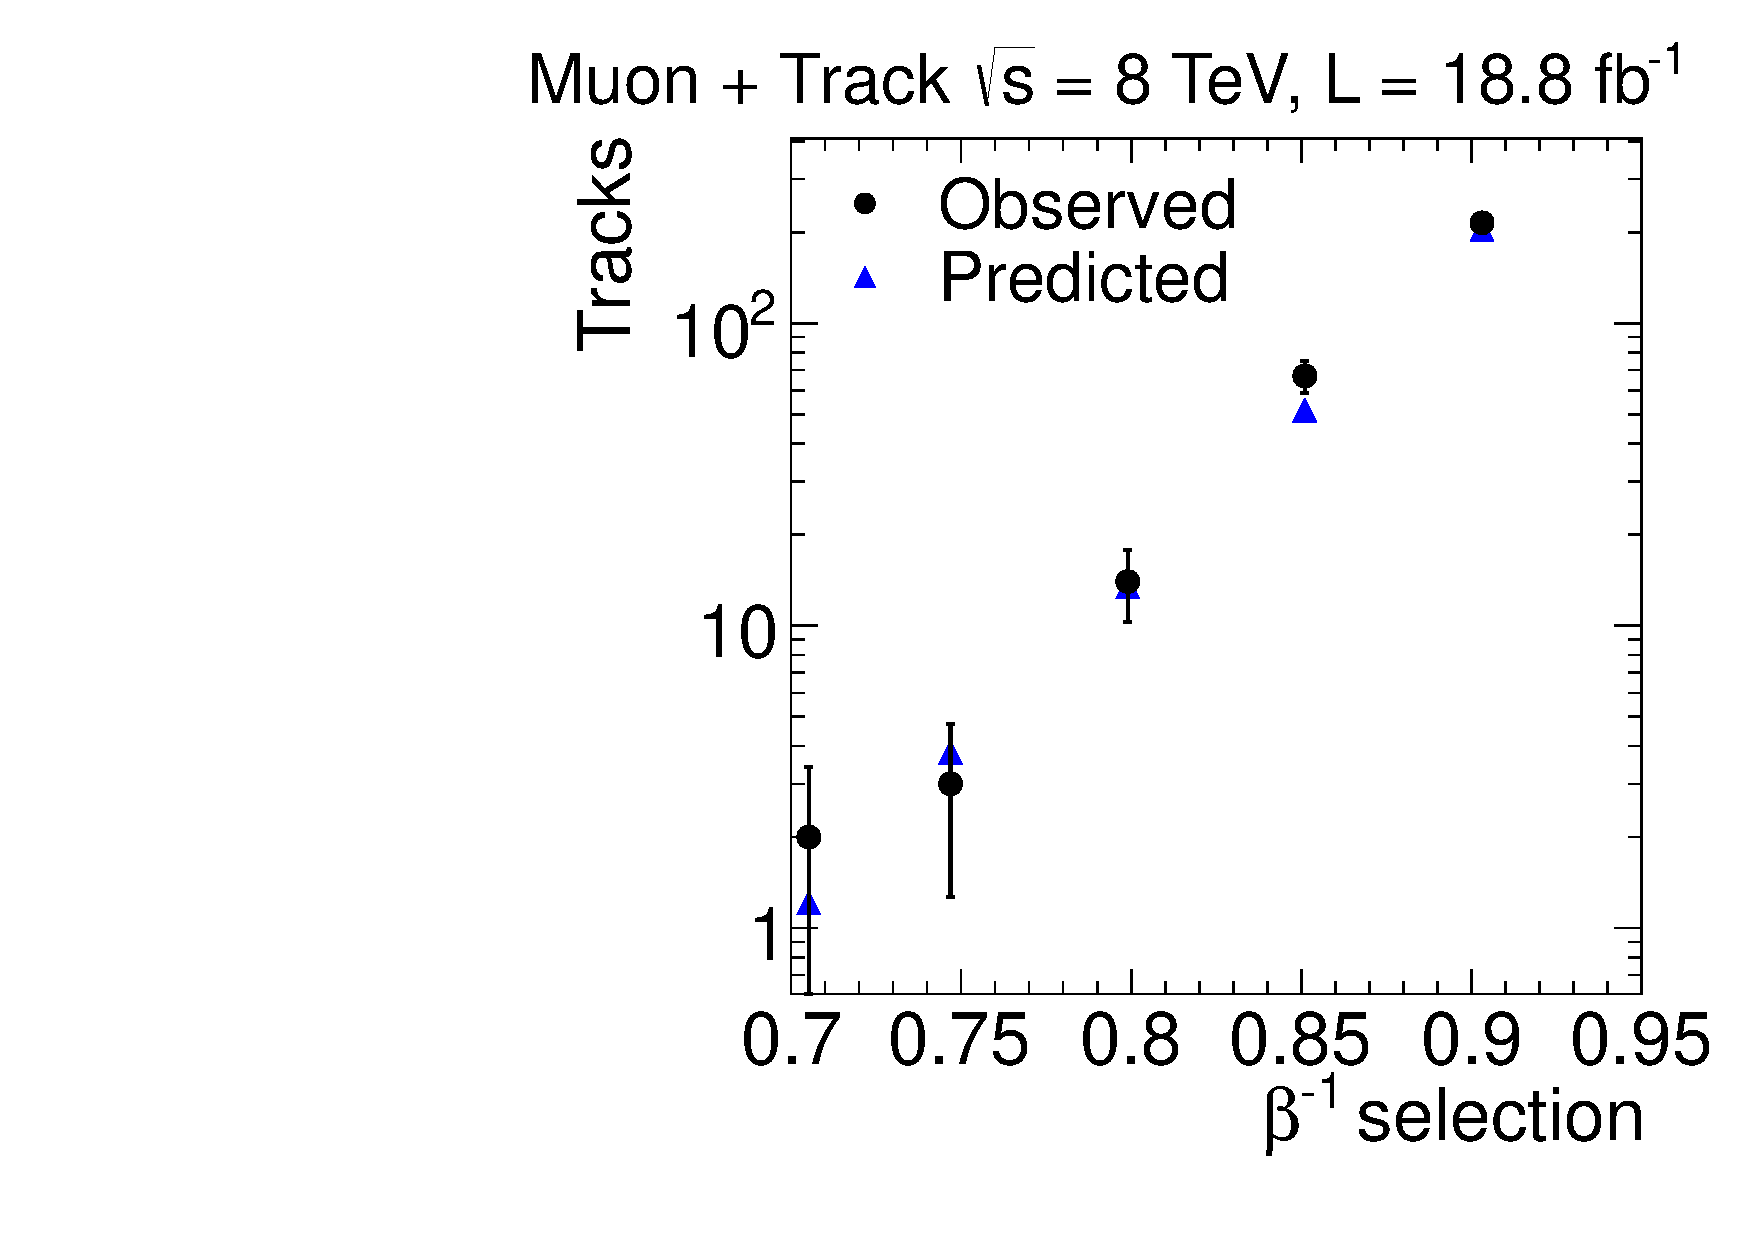
\includegraphics[clip=false, trim=0.0cm 0cm 0.0cm 0cm, width=0.48\textwidth]{figures/tkmu/Pred_Flip_I020_Pt85_Data8TeV}
\caption[Number of observed and predicted tracks in the \invbeta\ $<$ 1 region in the \tktof\ analysis.]
{Number of observed and predicted tracks and their statistical error in the $D^\prime$ region for a loose selection of $p_T>55$~GeV/$c$, $I_{as}>0.1$ (left)
and a tight selection of $p_T>85$~GeV/$c$, $I_{as}>0.2$ (right) in the \tktof\ analysis. The threshold on $1/\beta$ is defined by the x-axis.
Figures are cumulative, as tracks passing the selection with tight thresholds will also pass for loose thresholds.}
\label{fig:PredFlipTkTOF}
\end{center}
\end{figure}

In addition to the requirements on the selection variables, the \tktof\ analysis also applies a requirement on the estimated mass of the track as determined from 
Equation~\ref{eq:MassFromHarmonicEstimator}. In order to do this the mass spectrum of background tracks in the signal region must be predicted.
The background mass spectrum is predicted using the \dedx\ and momentum distributions taken from control regions. While the signal region is defined by thresholds on \ias\ and
$p_T$ (as well as \invbeta), the mass prediction uses \ih\ and $p$ so it is these distributions that must be taken from the control regions. 

It has been found that the probability for background tracks to pass the threshold on \ias\ is dependent on the $\eta$ of the track.
The probability to pass the \invbeta\ threshold has a small $\eta$
dependence while the probability to pass the $p_T$ threshold has almost no $\eta$ dependence. These effects can be seen in Figure~\ref{fig:etacorrelation} which shows the $\eta$
distribution of tracks which
pass or fail the various thresholds. 
This is found to have only a small effect on the total number of predicted tracks but does bias the predicted mass spectrum which uses $p$ instead of \pt.
%As discussed above the
%\dedx\ variables have a strong $\eta$ dependence. While this issue does not have a large effect on the total number of predicted tracks is does affect the mass distribution.
The $p_T$ distribution of background tracks is roughly the same for different values of $\eta$ 
however this implies that the $p$ distribution does vary, as momentum can be written
as a function of only $p_T$ and $\eta$. To correct for this a reweighting procedure is done such that the tracks
used to determine the $p$ distribution match the $\eta$ distribution of tracks used to obtain the $I_h$ distribution.

\begin{figure}
\begin{center}
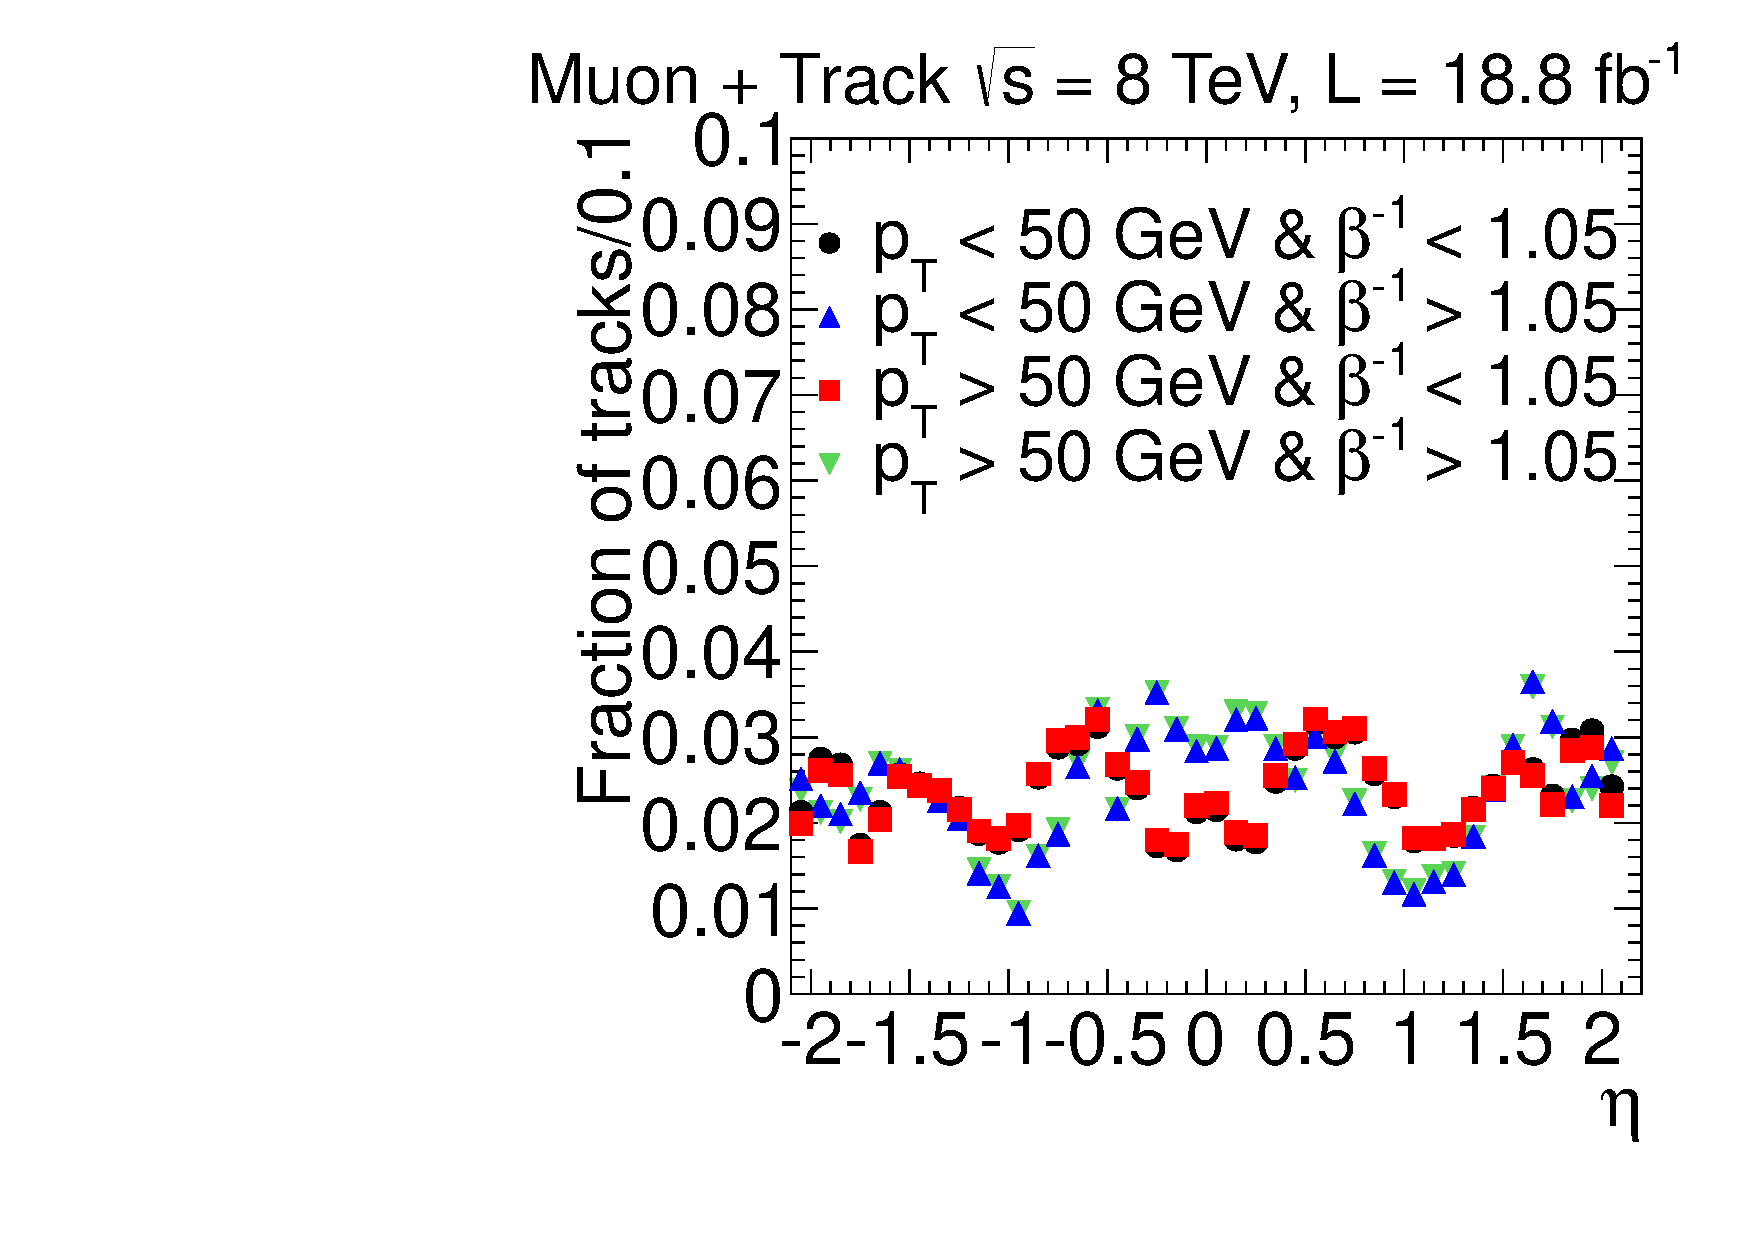
\includegraphics[clip=false, trim=0.0cm 0cm 0.0cm 0cm, width=0.48\textwidth]{figures/tkmu/Selection_Data8TeV_EtaRegionsPtTOF_016}
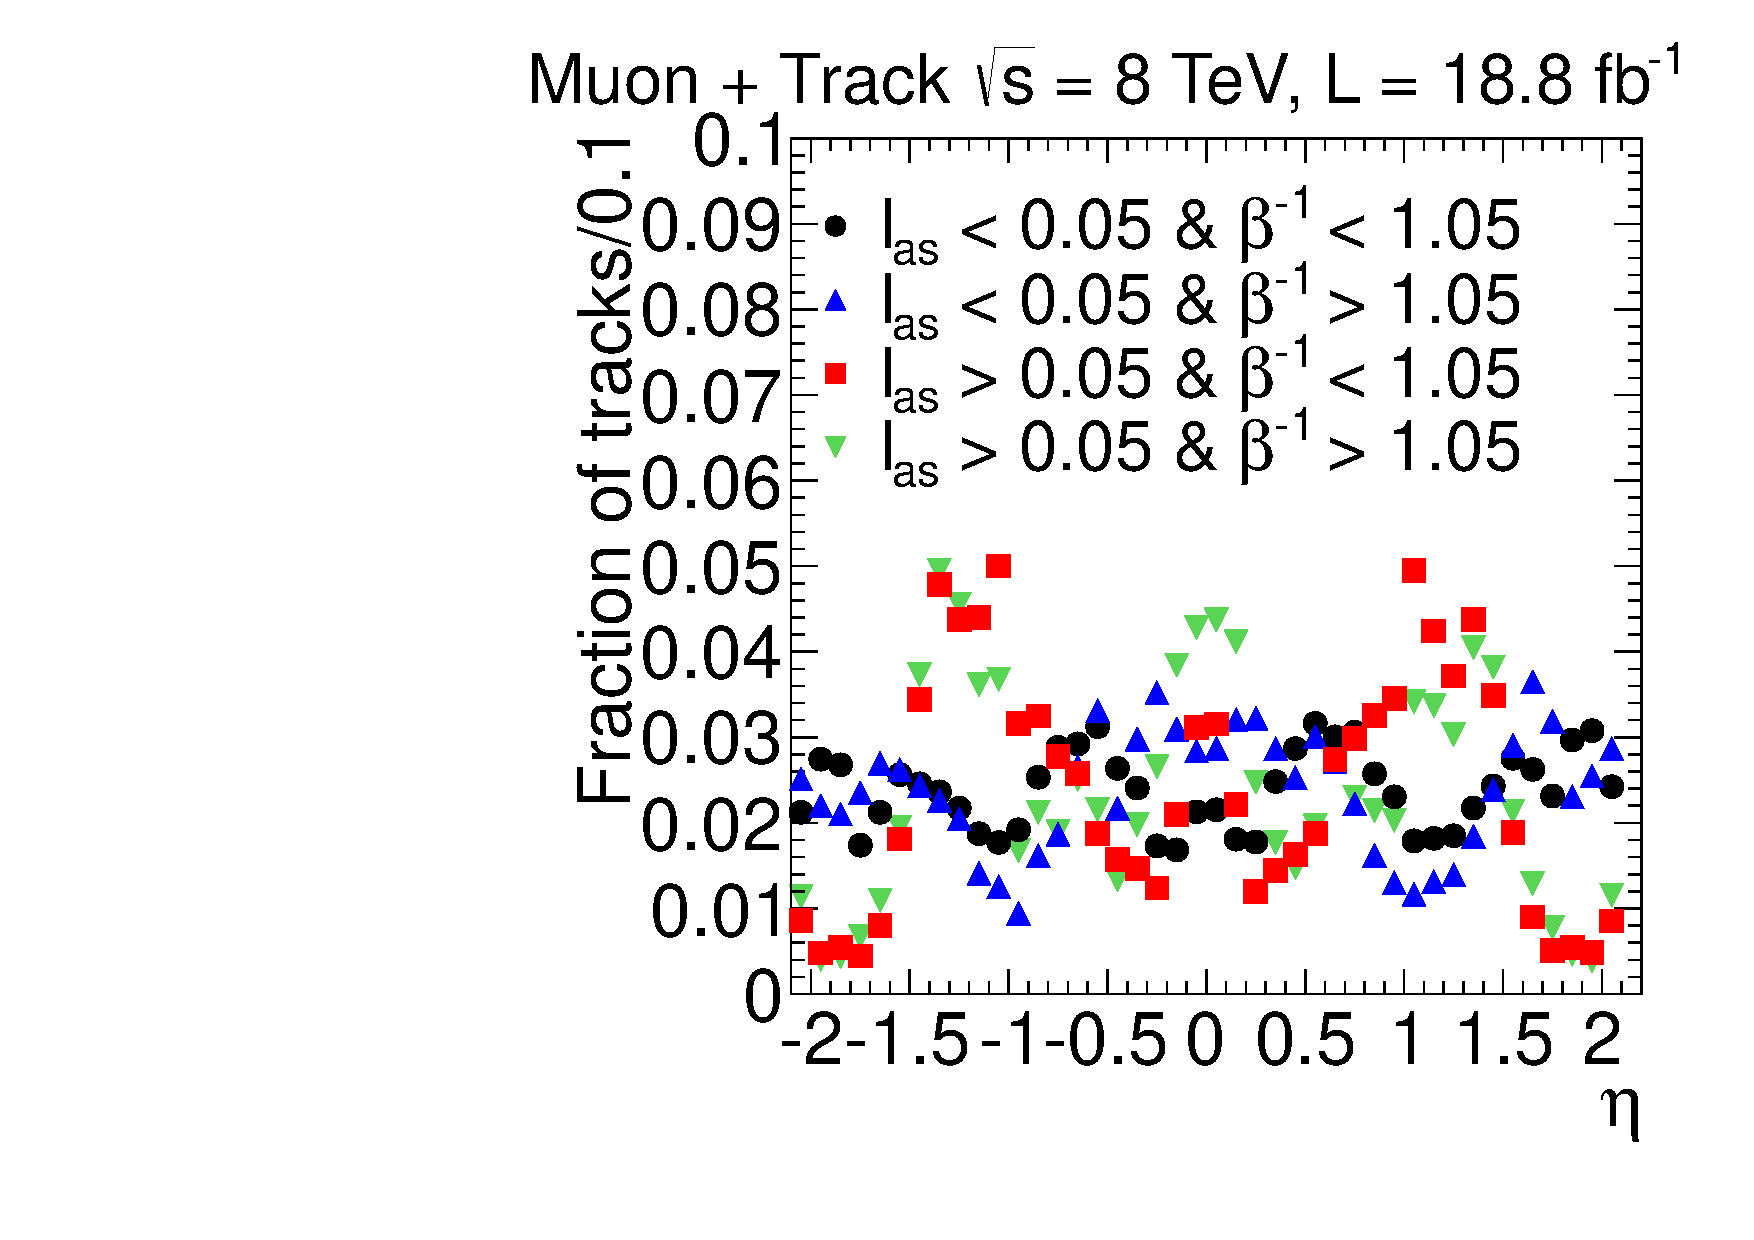
\includegraphics[clip=false, trim=0.0cm 0cm 0.0cm 0cm, width=0.48\textwidth]{figures/tkmu/Selection_Data8TeV_EtaRegionsTOFdEdx_016} \\
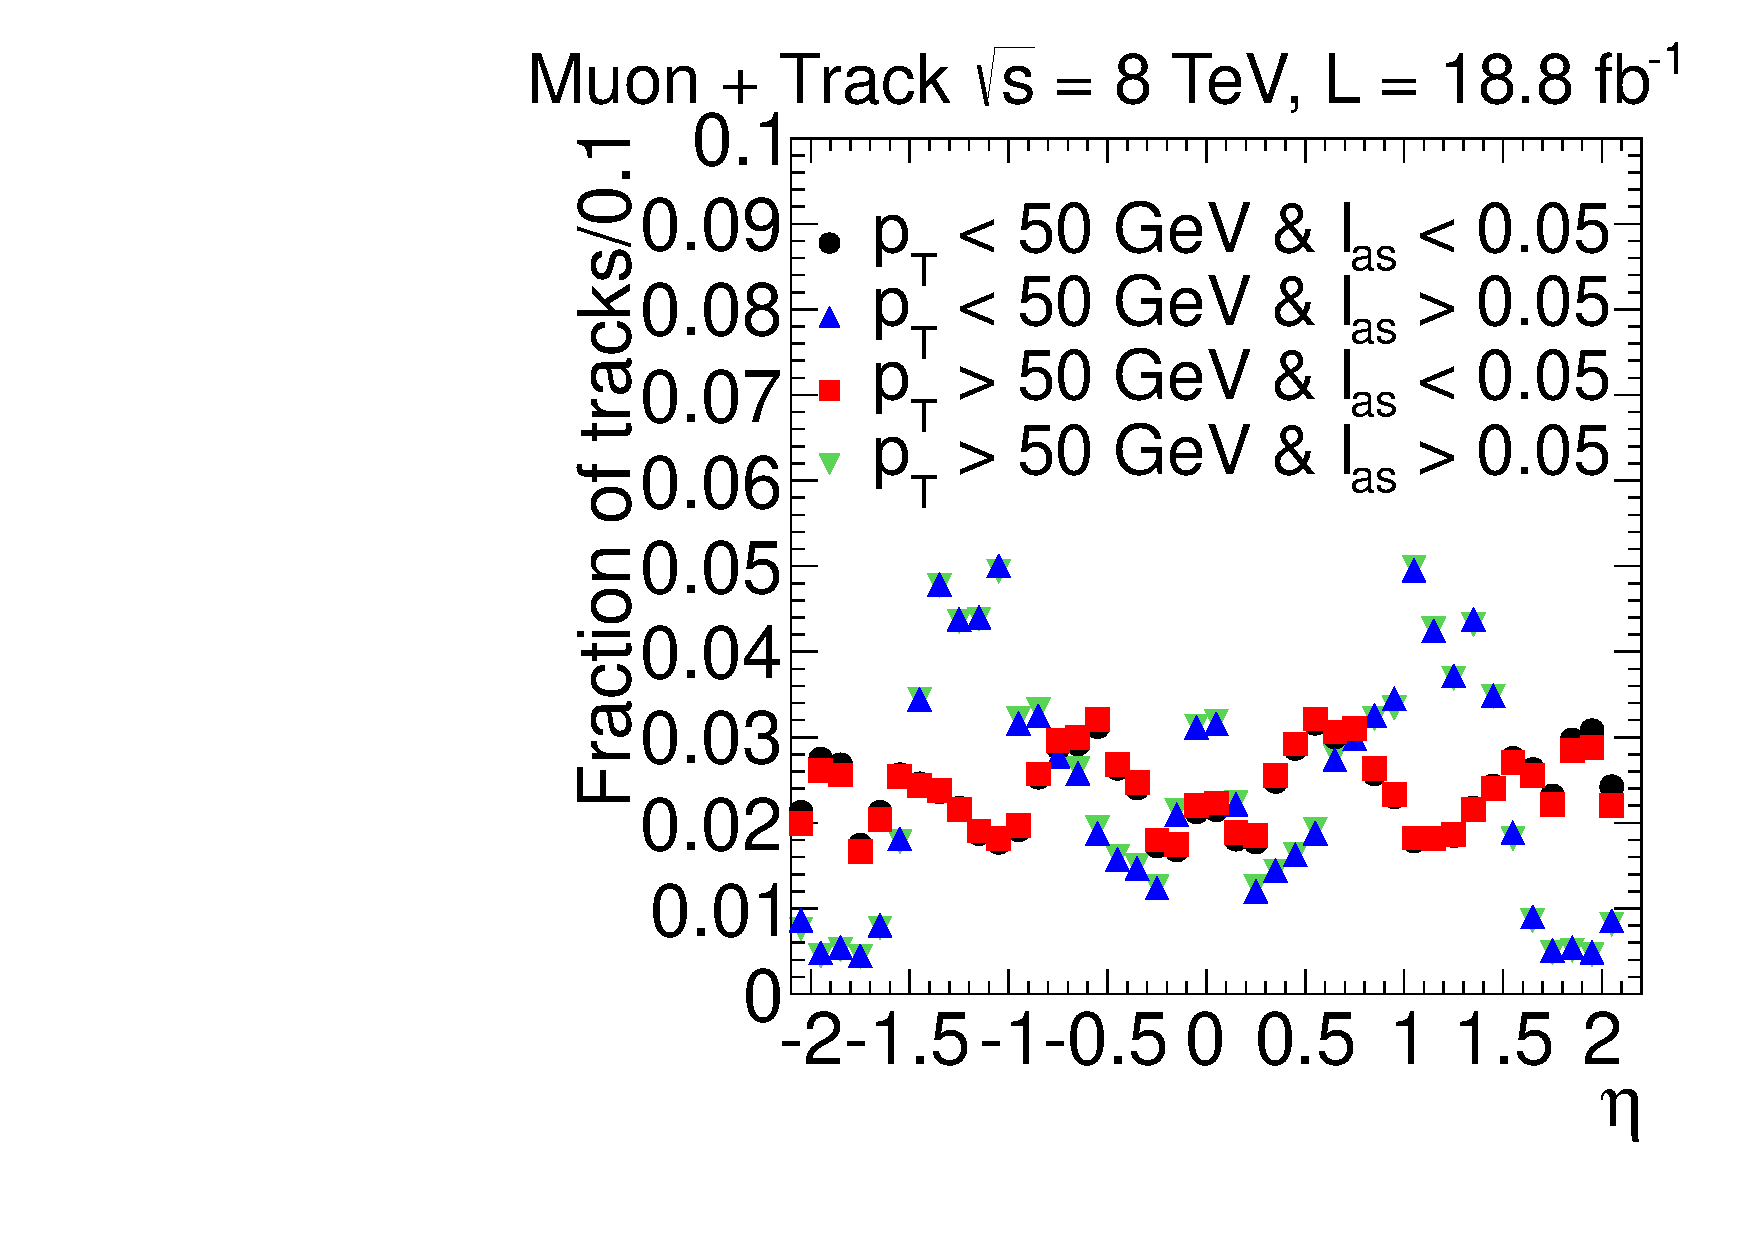
\includegraphics[clip=false, trim=0.0cm 0cm 0.0cm 0cm, width=0.48\textwidth]{figures/tkmu/Selection_Data8TeV_EtaRegionsPtdEdx_016}
\end{center}
\caption[Distribution for data of the track $\eta$ for various combinations of being above or below selection thresholds in the \tktof\ analysis]
{Distribution for data of the track $\eta$ for various combinations of being above or below selection thresholds of
50 GeV/$c$ for $p_T$, 1.05 for \invbeta, and 0.05 for \ias.
Top left: Combinations of flipping $p_T$ and \invbeta\ thresholds. Top Right: Combinations of flipping \invbeta\ and \ias\ thresholds.
Bottom: Combinations of flipping $p_T$ and \ias\ thresholds. For all plots the variable not flipped is required to be below the threshold.}
\label{fig:etacorrelation}
\end{figure}

%The prescription for determining the predicted background mass shape was done by another scientist working on CMS and is simply reproduced here.
The $p$ (\ih) distribution
is taken from the $G$ ($A$) region where only the $p_T$  (\ias), value is above threshold and the other two are below. The mass distribution is then predicted by performing
approximately 100 pseudo-experiments. The $i^{th}$ pseudo-experiment is done through multiple steps. First a value of $E_{i}$ ($F_i$) is drawn from a Poisson
distribution with a mean equal to the observed number of tracks in the $E$ ($F$) regions in data.
Next, a binned distribution is created from the $p$ of tracks in the $G$ region. A value of $n_{ij}$, where j represents the bin of the $p$ distribution, is drawn for
each $p$ bin from a Poisson distribution with mean equal to the number of tracks observed in that bin in data. A value of $G_i$ is then found as the sum over j of the
$n_{ij}$. A similar procedure is done in the $A$ region for determining the \ih\ distribution. Before the distribution is found, 
the tracks in the $A$ region are binned by $\eta$ using a bin width of 0.1. Weights are attached to the tracks in a bin equal to the number of tracks in the
same $\eta$ bin in the $G$ region divided by the number of tracks in the bin in the $A$ region. This corrects for the $\eta$ dependence discussed above.
Next, a value of $m_{ik}$ is found for each bin of the reweighted \ih\ distribution. A value of $A_i$ is then found by summing $m_{ik}$ over k.
The predicted number of background tracks in the signal region for a given j--k bin in the $p$ -- \dedx\ plane, $D_{ijk}$, is then found via the relation

\begin{equation}
D_{ijk} = (A_i \times F_i \times G_i / E_{i}^{2}) \times (n_{ij}/G_i) \times (m_{ik}/A_i) = F_i \times n_{ij} \times m_{ik} / E_{i}^{2}
\label{eq:MassPrediction}
\end{equation}

The predicted tracks in $D_{ijk}$ are taken to have a mass equal to the mass coming from Equation~\ref{eq:MassFromHarmonicEstimator} with the $p$ and \ih\ values
determined by the bin that $j$ and $k$ represent in the $p$ and \ih\ distributions, respectively. The mass distribution for the $i^{th}$ pseudo-experiment is then
found by summing $D_{ijk}$, with its representative mass, over $j$ and $k$.

The value in each mass bin is then found as the average of the value in all the pseudo-experiments. The statistical error is taken as the standard deviation of the values from
the pseudo-experiments.

As the \invbeta\ value of tracks is not currently used in the mass estimation the predicted and observed mass spectrums in the \invbeta\ $<$ 1 region can be
found by only changing the groups that the tracks be drawn from be the regions with a prime (e.g. $A^\prime$). Using the \invbeta\ $<$ 1 region allows for checking
the predicted mass distribution in a background dominated region even when applying tight thresholds. The predicted and observed mass distributions are shown in 
Figure~\ref{fig:FlipMassDistribution} with both loose and tight thresholds on the selection variables.

\begin{figure}
 \begin{center}
  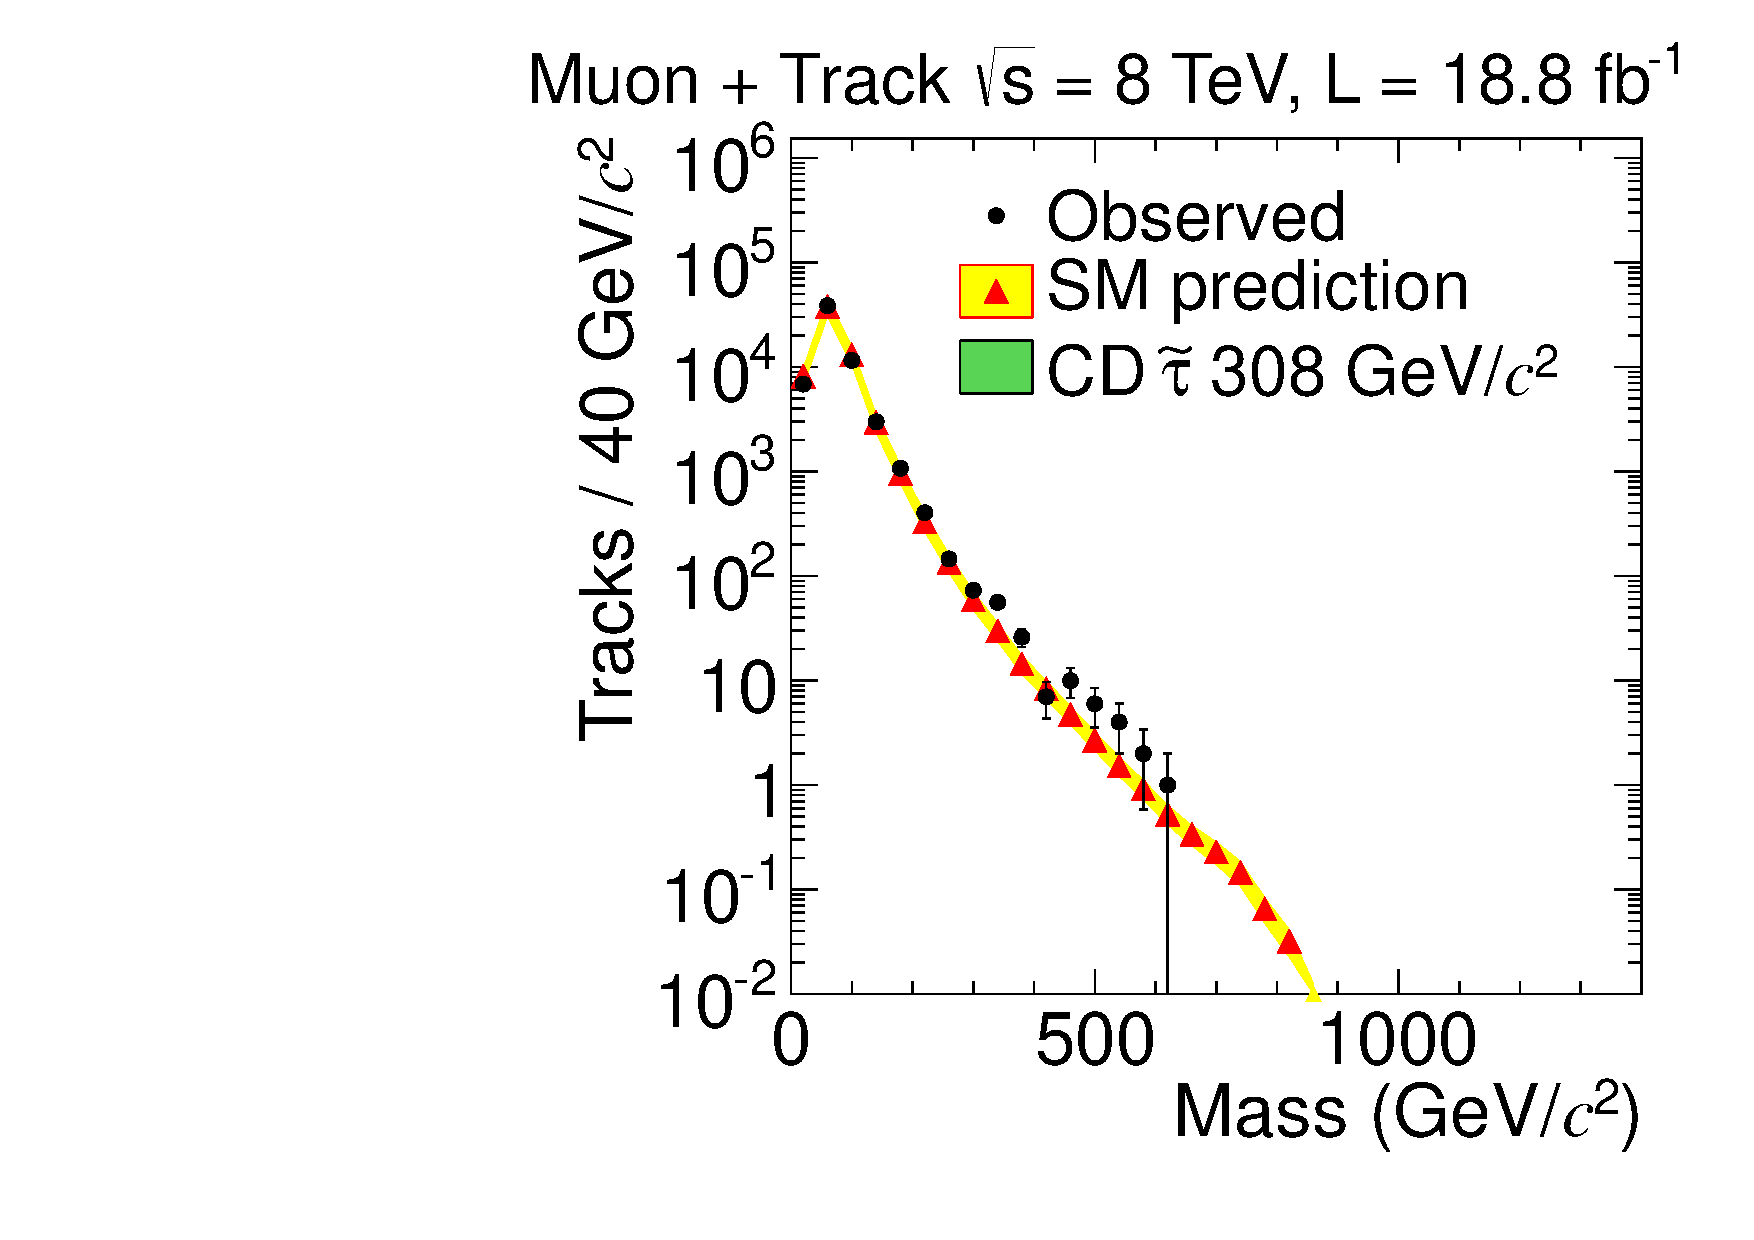
\includegraphics[clip=false, trim=0.0cm 0cm 0.0cm 0cm, width=0.48\textwidth]{figures/tkmu/RescaleNoRatio_Mass_Flip_8TeV_LooseNoSMMC}
  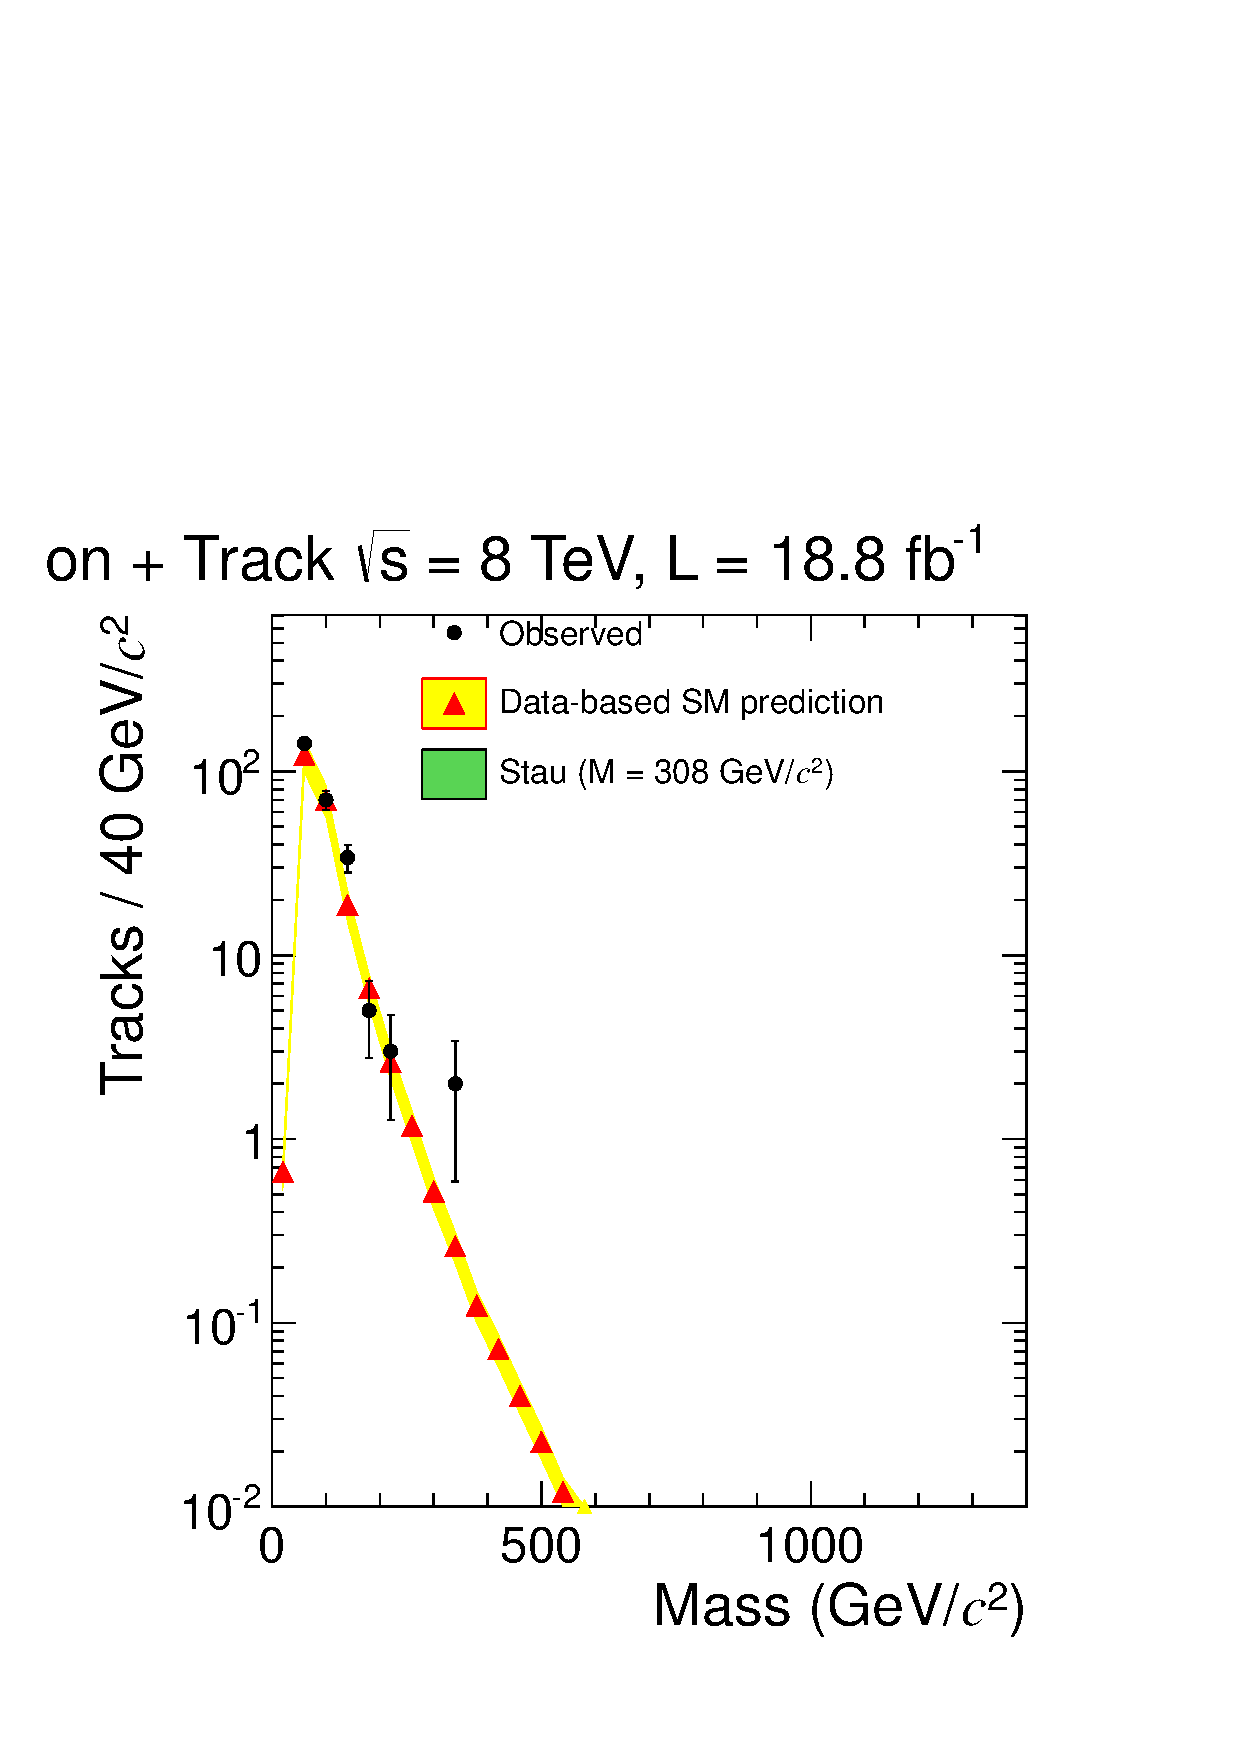
\includegraphics[clip=false, trim=0.0cm 0cm 0.0cm 0cm, width=0.48\textwidth]{figures/tkmu/RescaleNoRatio_Mass_Flip_8TeV_TightNoSMMC}
 \end{center}
 \caption[Observed and predicted mass spectrum for tracks in the \invbeta\ $<$ 1 region in the \tktof\ analysis.]
{Observed and predicted mass spectrum for tracks in the $D^\prime$ region in the \tktof\ analysis.
Left: Thresholds of $p_T > 55$ GeV/$c$, $I_{as} > 0.1$ and $1/\beta < 0.95$.
Right: Thresholds of $p_T > 85$ GeV/$c$, $I_{as} > 0.1$ and $1/\beta < 0.8$.
The error bands are only statistical.}
\label{fig:FlipMassDistribution}
\end{figure}

The systematic uncertainty on the background prediction for the \tktof\ analysis is evaluated by using the multiple different predictions possible when using the
three dimensional variation of the $ABCD$ method. As mentioned above, in addition to the chosen prediction of $A\times F\times G/E^2$, 
there are three more equations that can be used to predict the amount of background in the signal region with relatively small statistical uncertainty.
Those three are $A \times H/E$, $B \times G/E$, and $F \times C/E$.
%The chosen prediction includes the bin where all the variables are below the threshold ($E$) and the three where exactly one threshold is passed ($F$, $G$, and $G$).
%The three additional predictions include the group where all the thresholds are failed, one of the bins where exactly one threshold is passed,
%and one of the bins where exactly two of the thresholds are passed.

The three additional background predictions each test the correlation between two of the three selection variables. Here the prediction $A \times H/E$ is used as an example but
the argument is the same for the other predictions. Comparing $A \times H/E$ with the chosen background prediction of $A\times F\times G/E^2$ it can be seen that
the difference is replacing $F\times G/E$ with $H$. The $E$ group fails all three thresholds, the $F$ and $G$ groups pass only the \invbeta\ and $p_T$ thresholds,
respectively, and the $H$ group passes the \invbeta\ and $p_T$ thresholds but not \dedx. If \invbeta\ and $p_T$ are uncorrelated then the equation $F\times G/E$ should
predict the number of tracks in the $H$ region. So a comparison of the two predictions will test how well the assumption that the variables are uncorrelated works.
Likewise, the prediction $B \times G/E$ ($F \times C/E$) tests for possible correlation between $p_T$ and \dedx\ (\invbeta\ and \dedx).

The number of predicted tracks coming from the four predictions is shown in Figure~\ref{fig:TkMuMultPred}. The spread of the four predictions is used to extract 
the systematic through Equation~\ref{eq:variance} with N=4. The statistical and systematic uncertainties are shown in Figure~\ref{fig:TkMuUnc}. From the last plot
and the agreement in the predicted mass spectrum a conservative systematic uncertainty of 20\% is taken.

\begin{figure}
 \begin{center}
  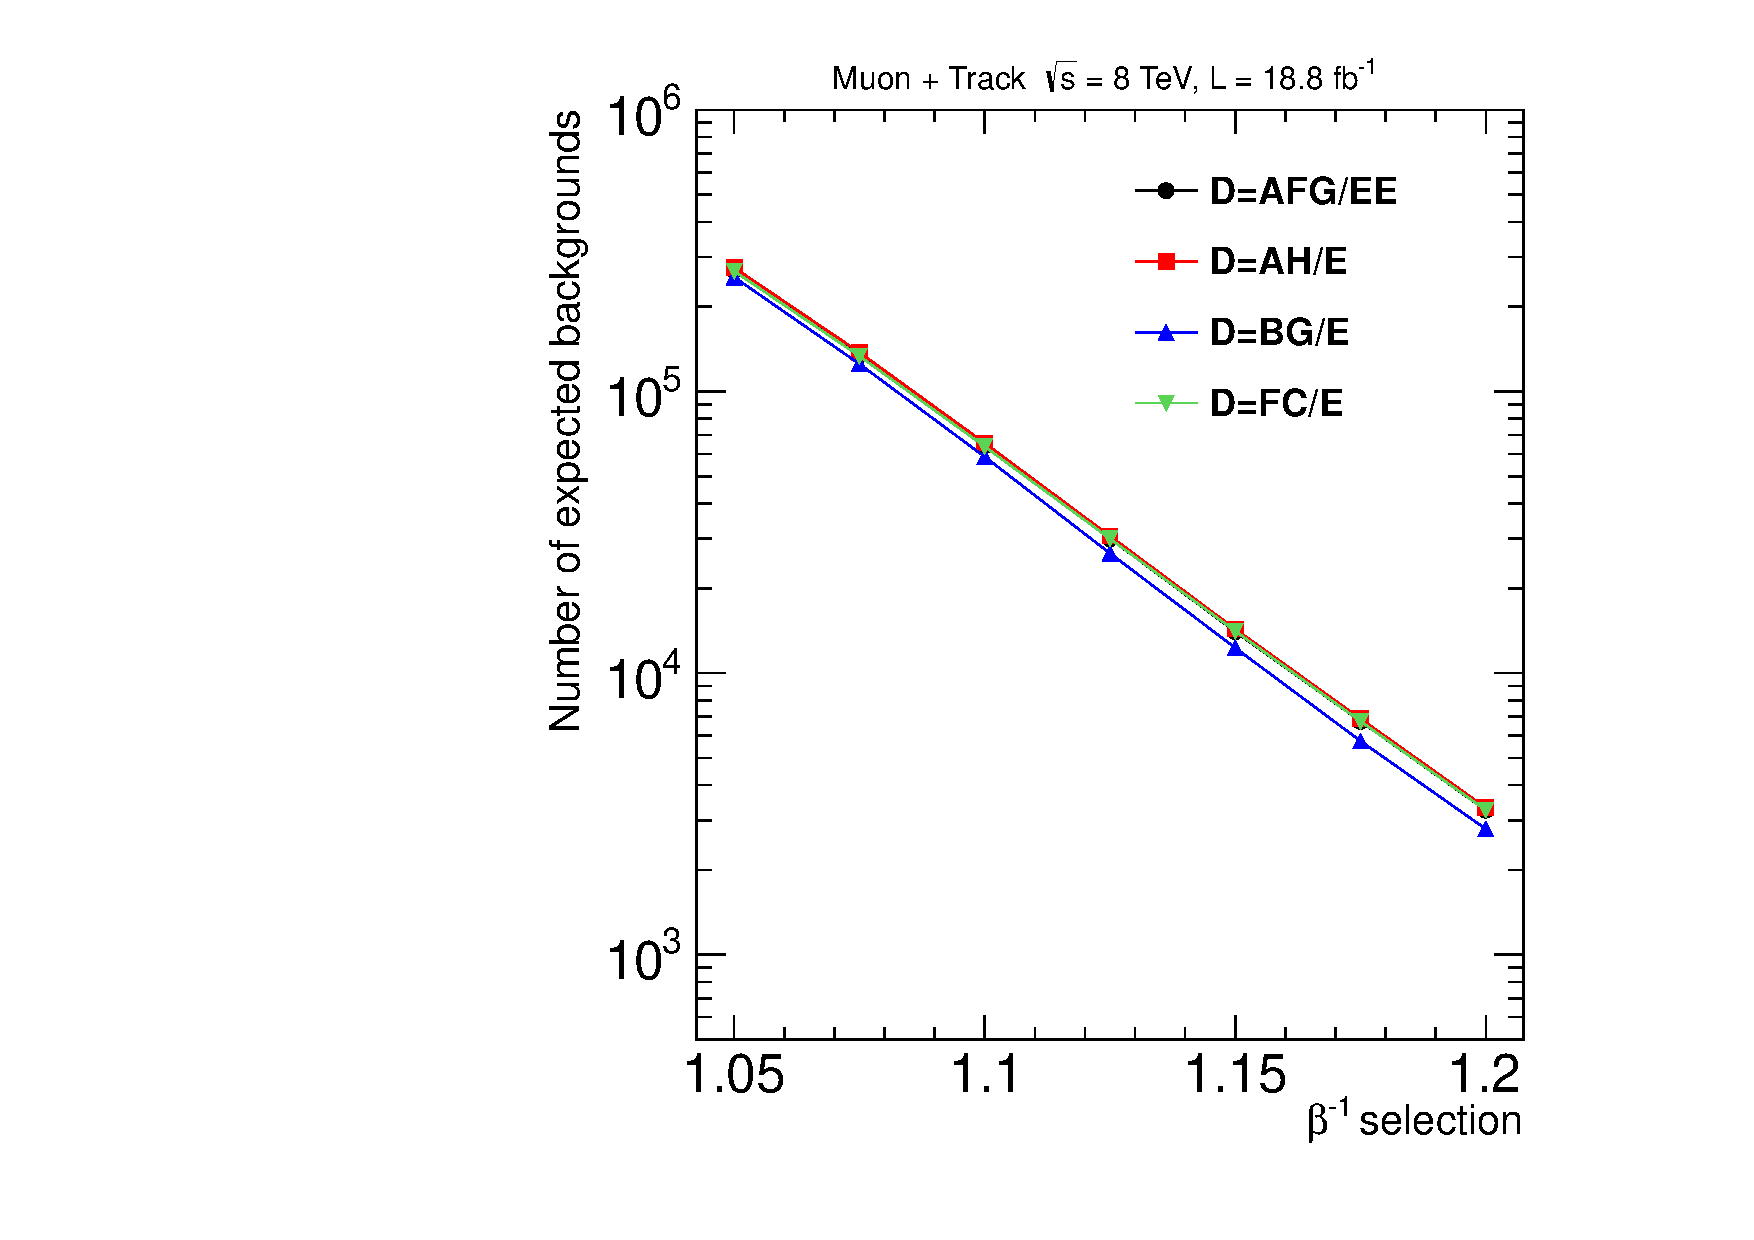
\includegraphics[clip=false, trim=0.0cm 0cm 0.0cm 0cm, width=0.48\textwidth]{figures/tkmu/Systematics_Data8TeV_TOF_Value}
  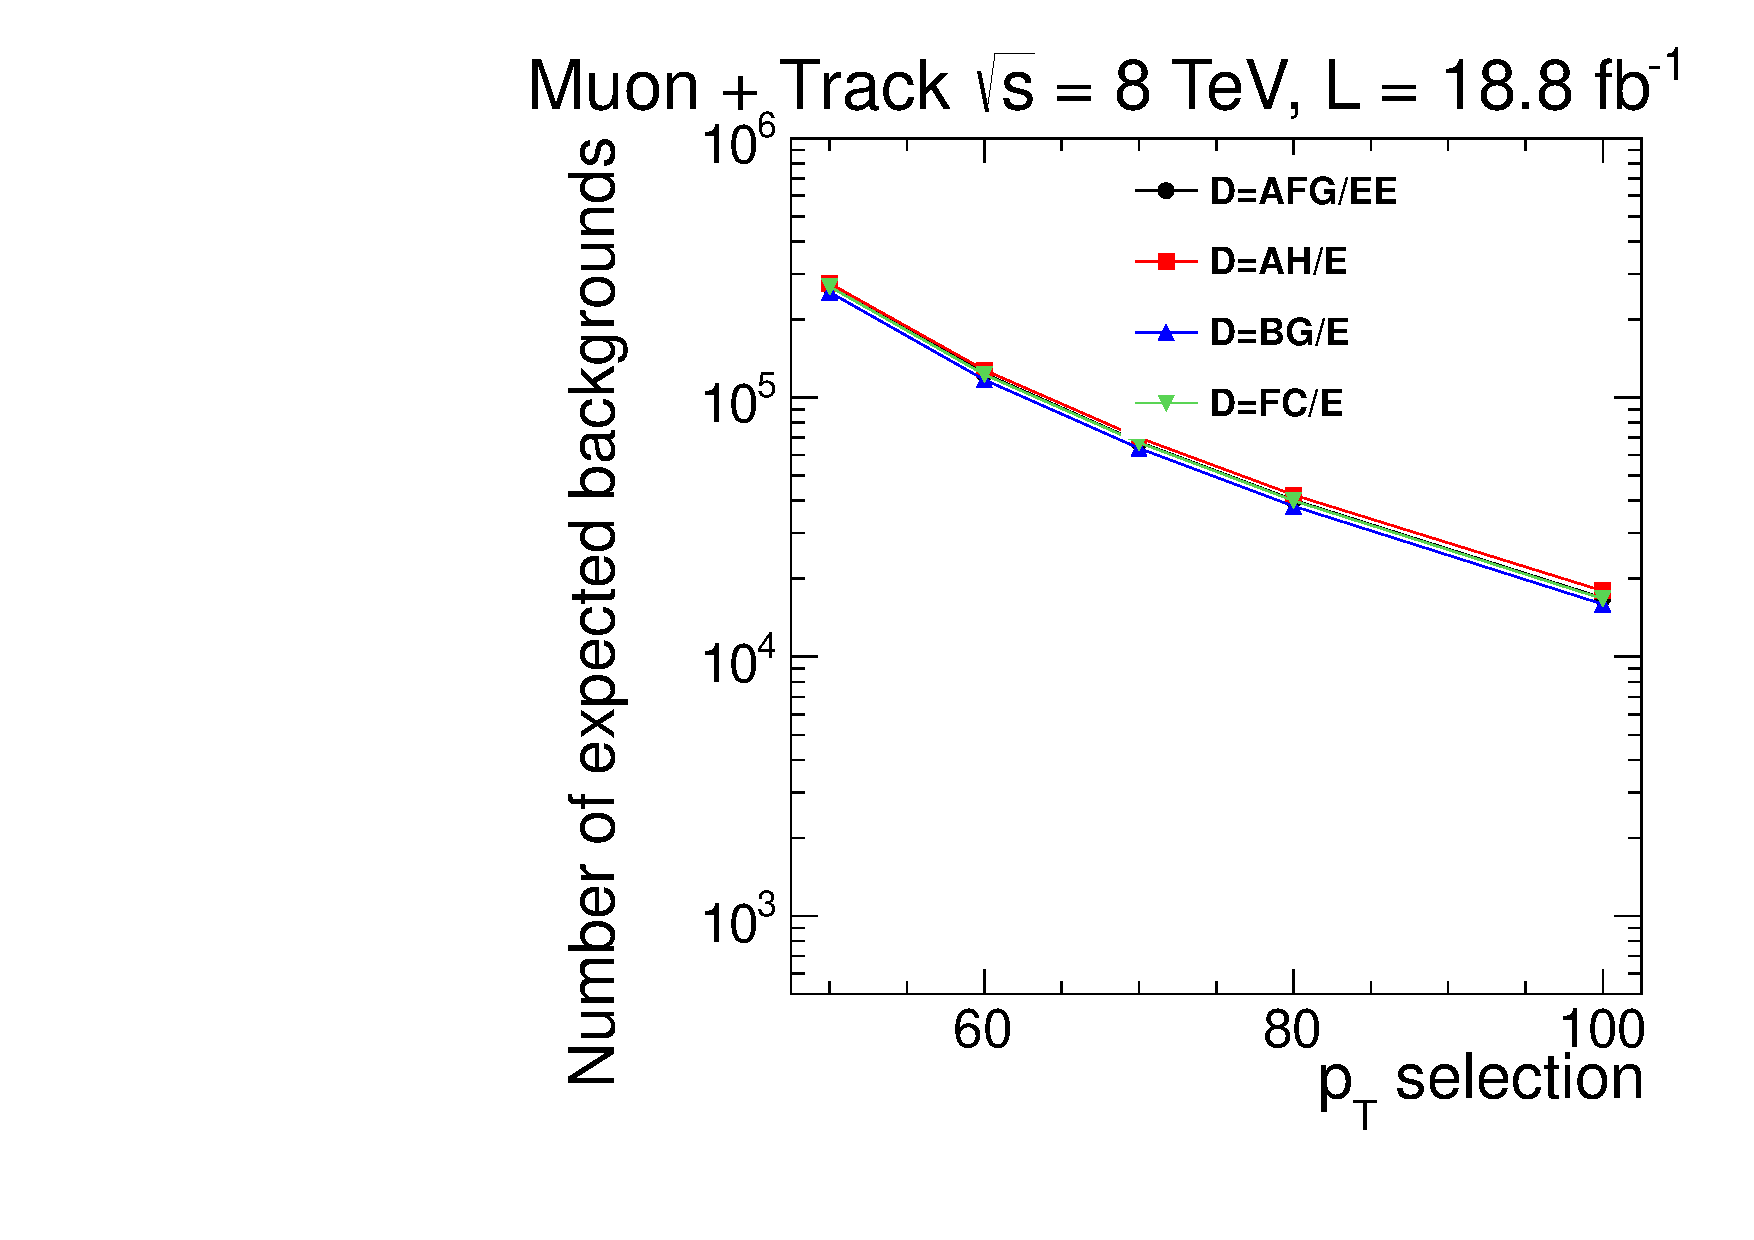
\includegraphics[clip=false, trim=0.0cm 0cm 0.0cm 0cm, width=0.48\textwidth]{figures/tkmu/Systematics_Data8TeV_P_Value} \\
  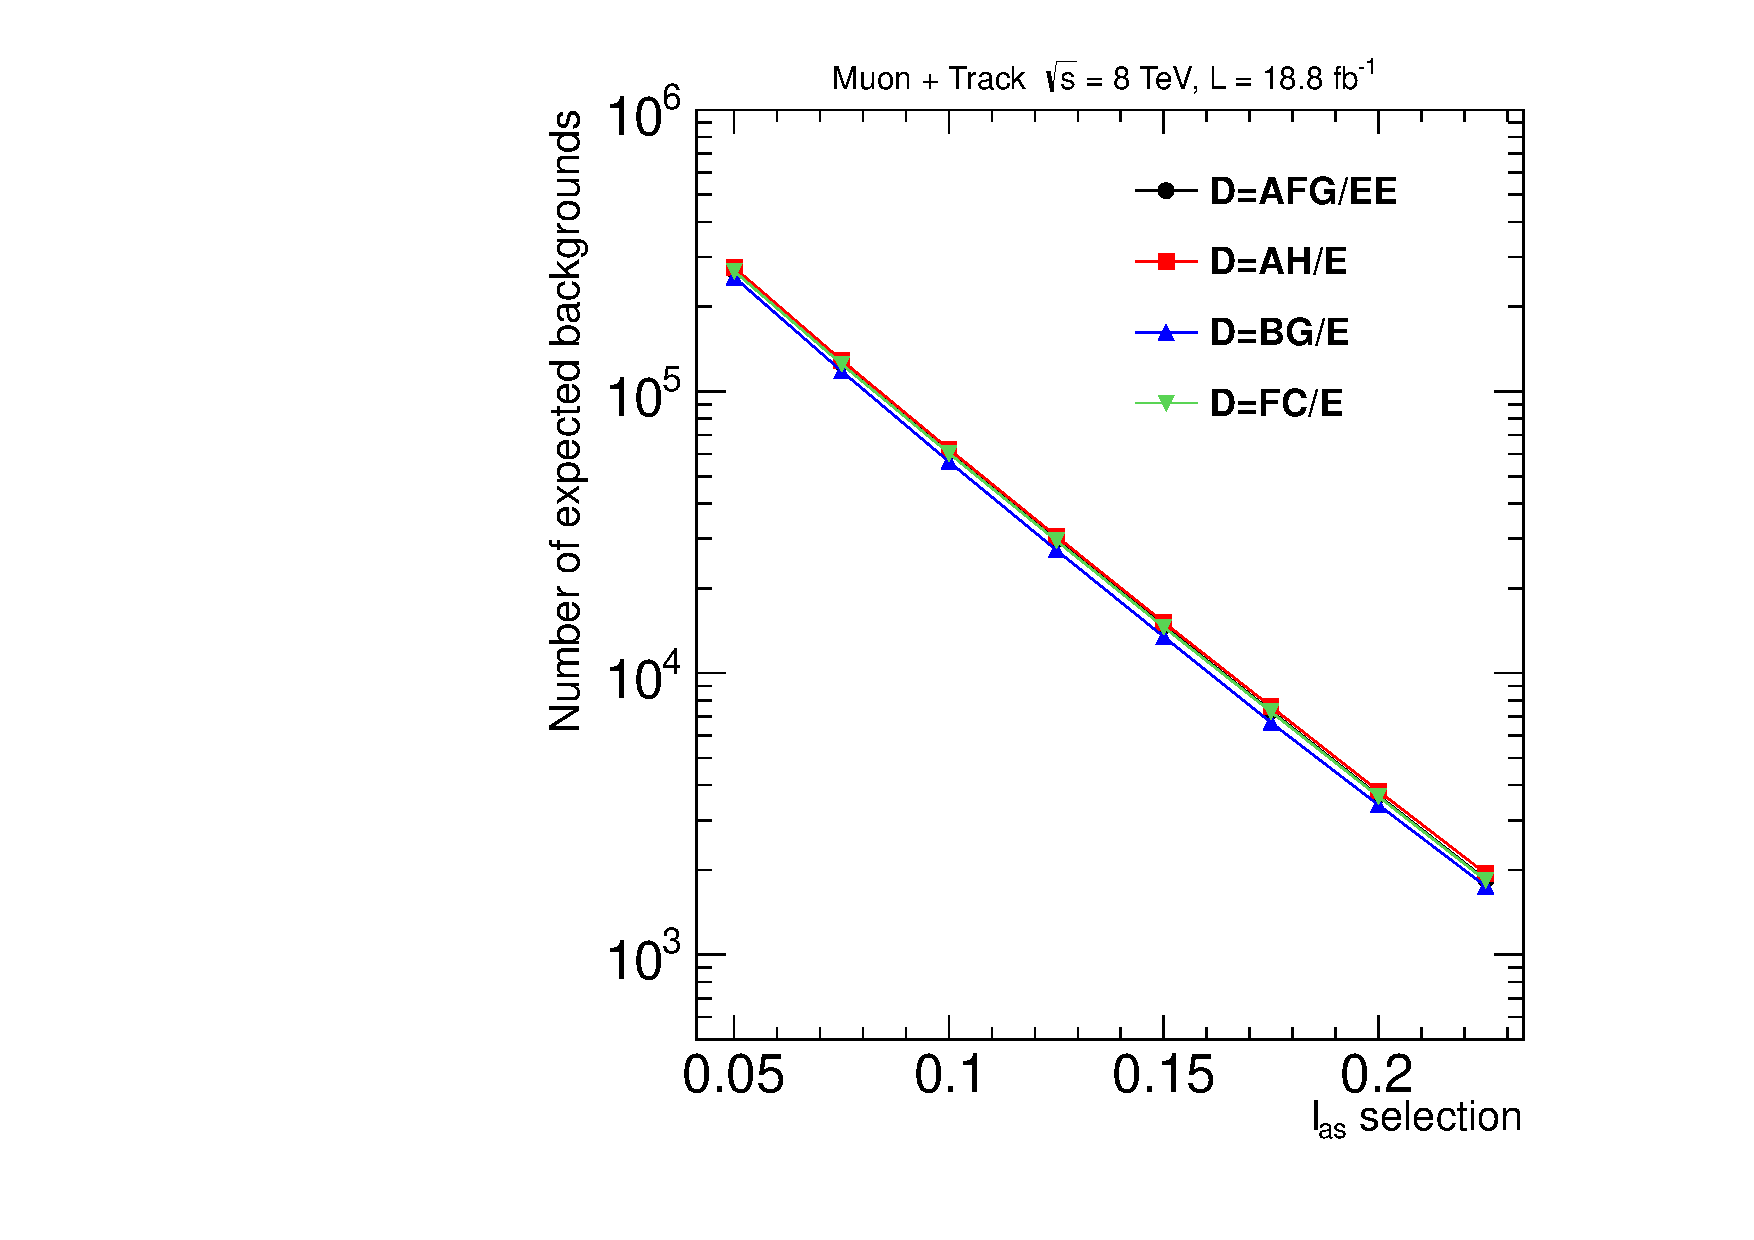
\includegraphics[clip=false, trim=0.0cm 0cm 0.0cm 0cm, width=0.48\textwidth]{figures/tkmu/Systematics_Data8TeV_I_Value}
 \end{center}
 \caption[Number of predicted tracks from four different background predictions in the \tktof\ analysis]
{Number of predicted tracks from four different background predictions in the \tktof\ analysis. 
Figures are cumulative, as tracks passing the selection with tight thresholds will also pass for loose thresholds.
Top Left: $p_T$ and \ias\ threshold of 50 GeV/$c$ and 0.05, respectively.
Threshold on \invbeta\ set by x-axis. Top Right: Threshold on \invbeta\  and \ias\ of 1.05 and 0.05, respectively. Threshold on $p_T$ set by x-axis.
Bottom: Threshold on \invbeta\ and $p_T$ of 1.05 and 50 GeV/$c$, respectively. Threshold on \ias\ set by x-axis. }
\label{fig:TkMuMultPred}
\end{figure}

\begin{figure}
\begin{center}
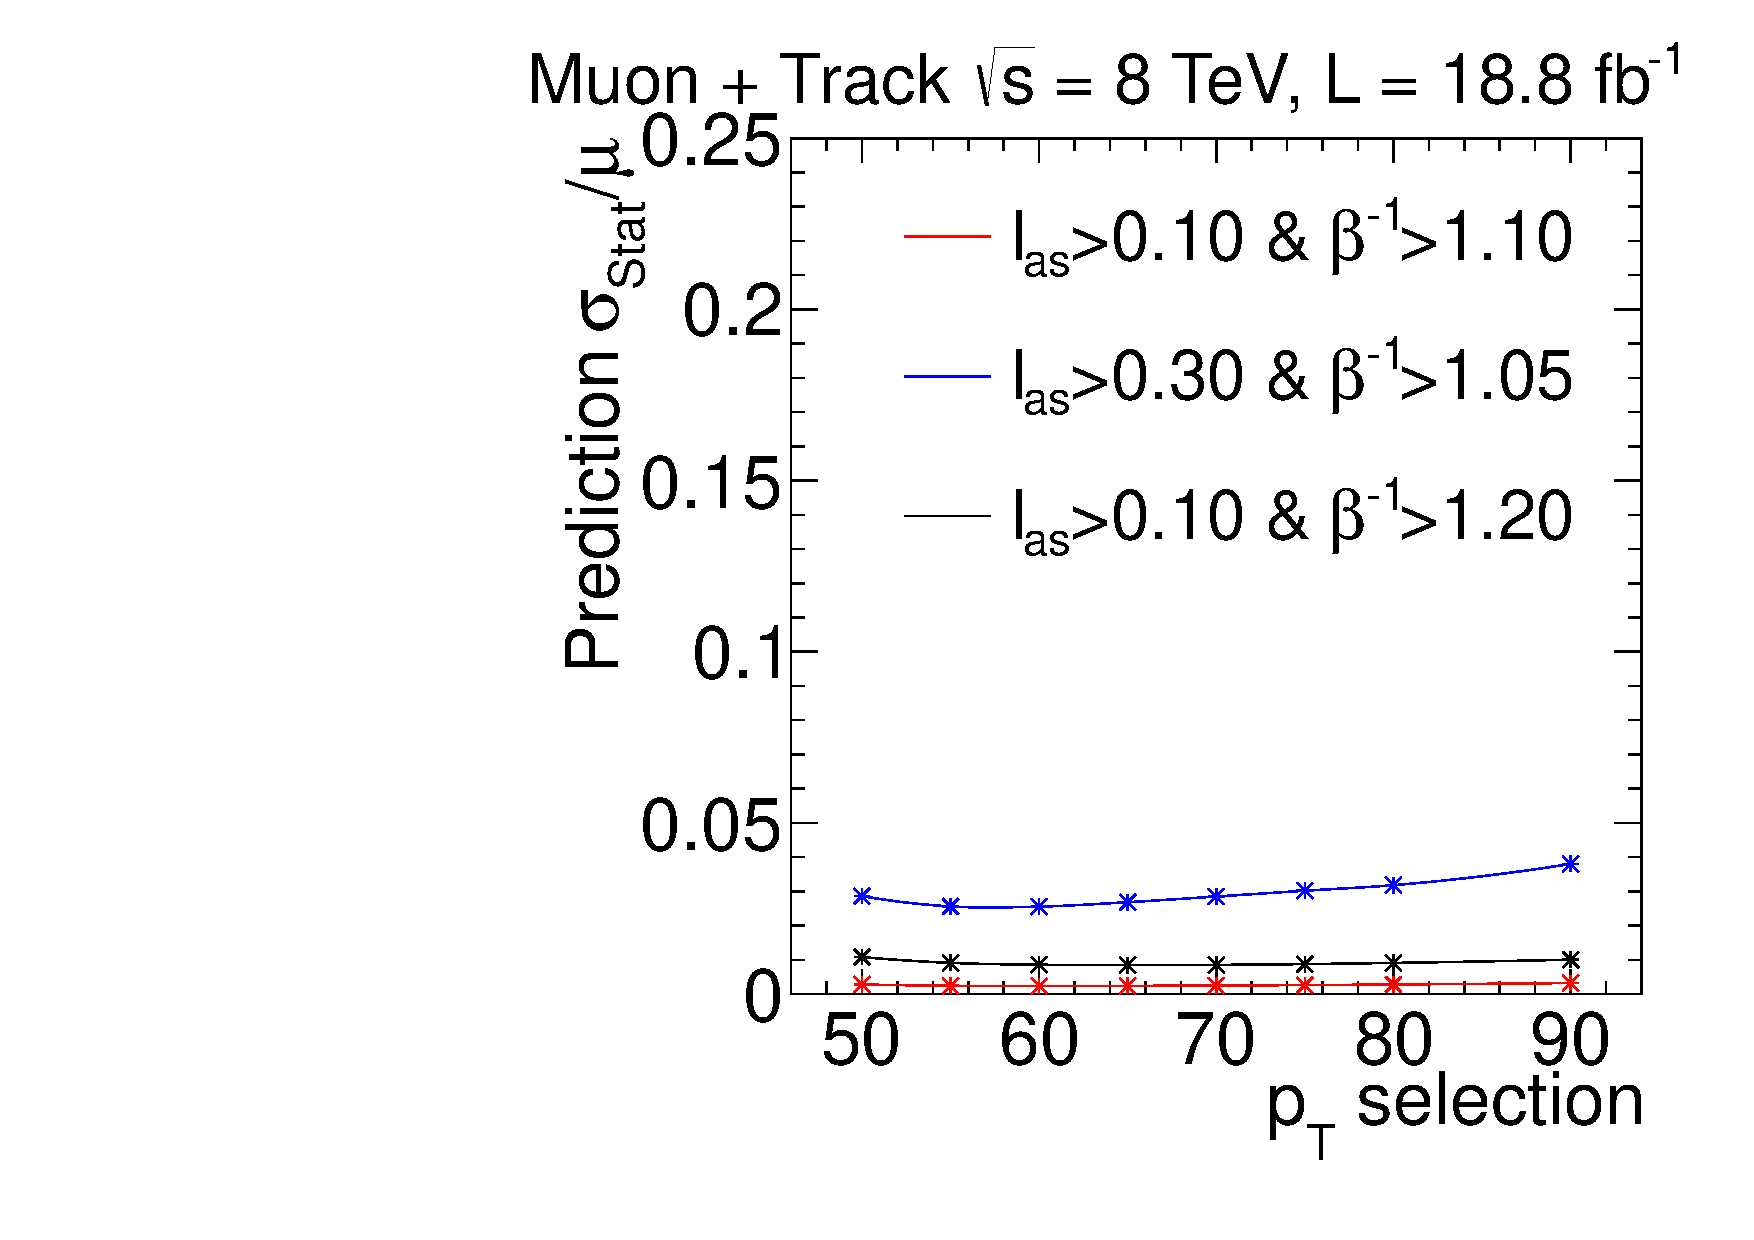
\includegraphics[clip=false, trim=0.0cm 0cm 0.0cm 0cm, width=0.48\textwidth]{figures/tkmu/Systematics_Data8TeV_pT_Stat}
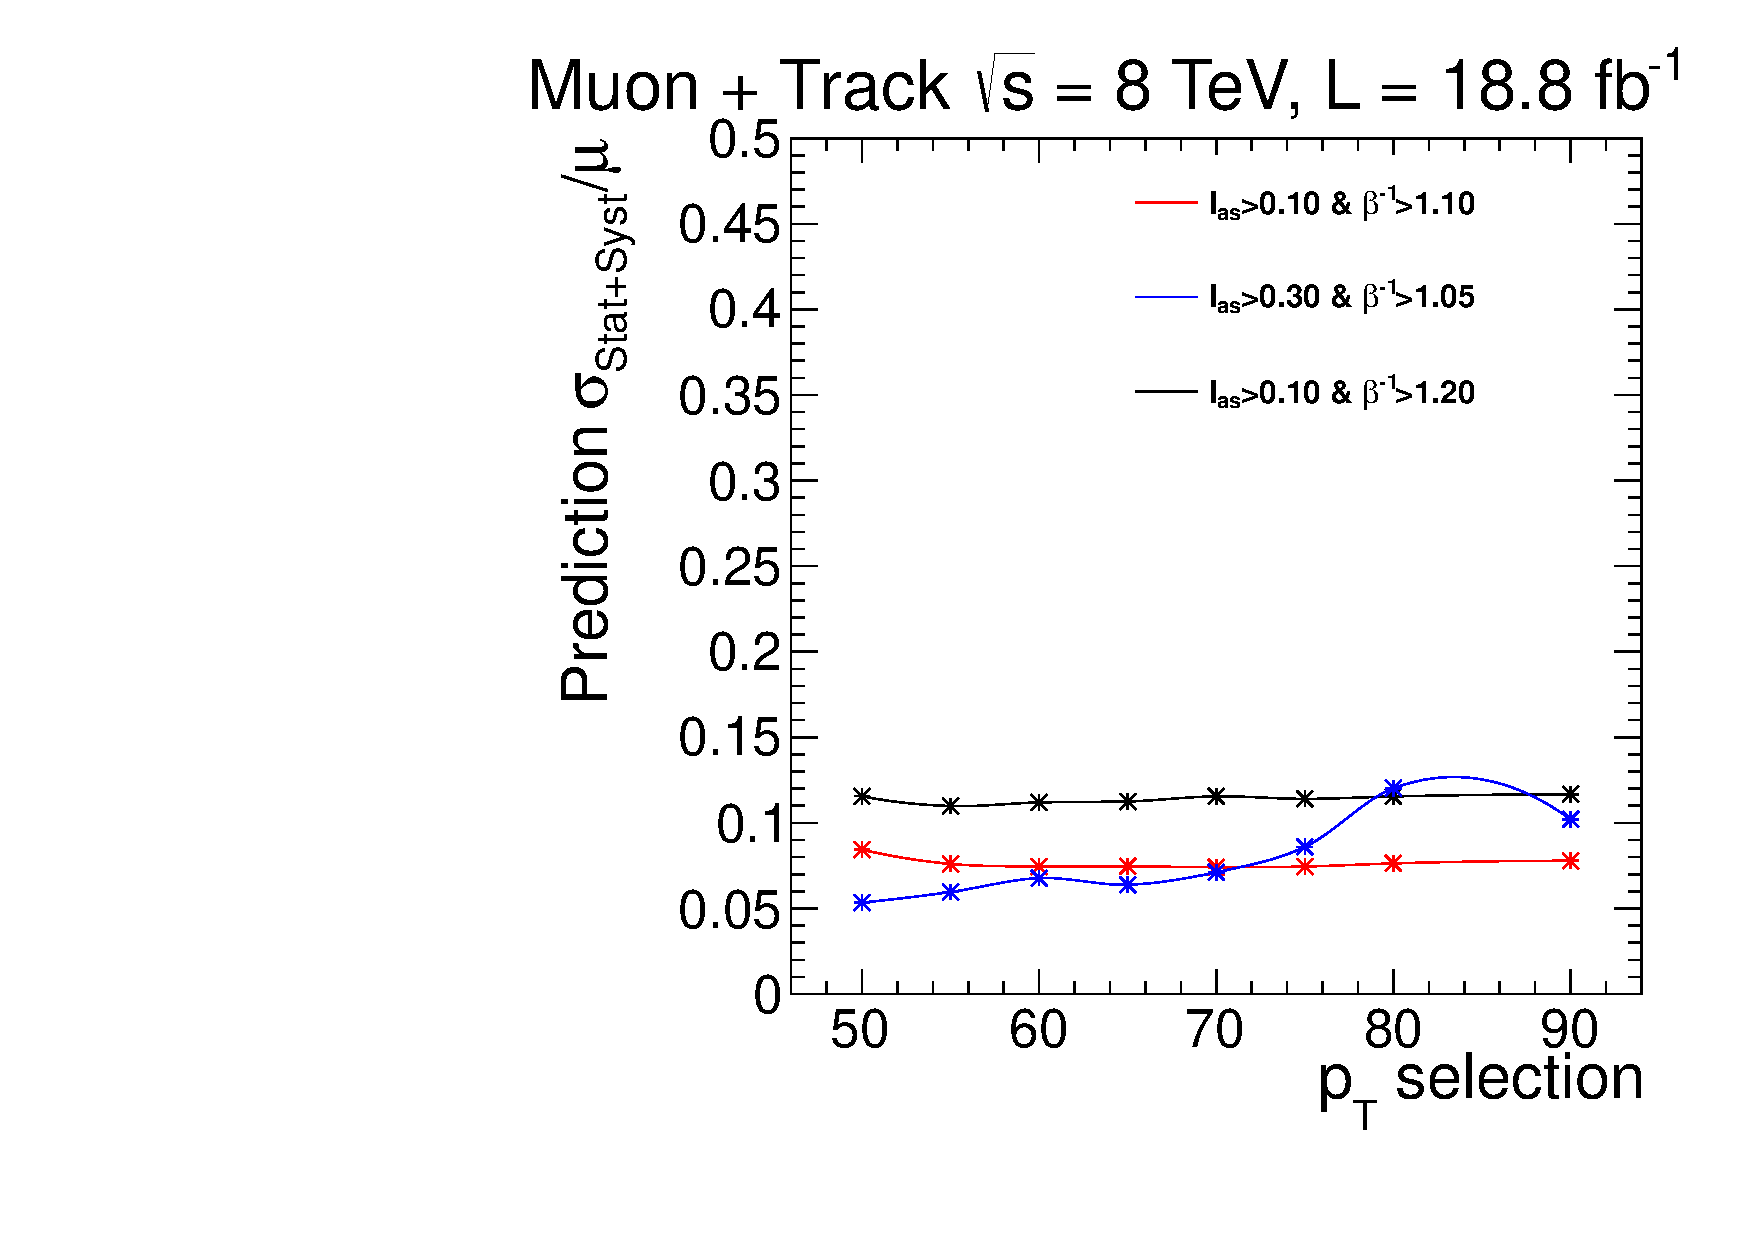
\includegraphics[clip=false, trim=0.0cm 0cm 0.0cm 0cm, width=0.48\textwidth]{figures/tkmu/Systematics_Data8TeV_pT_Sum} \\
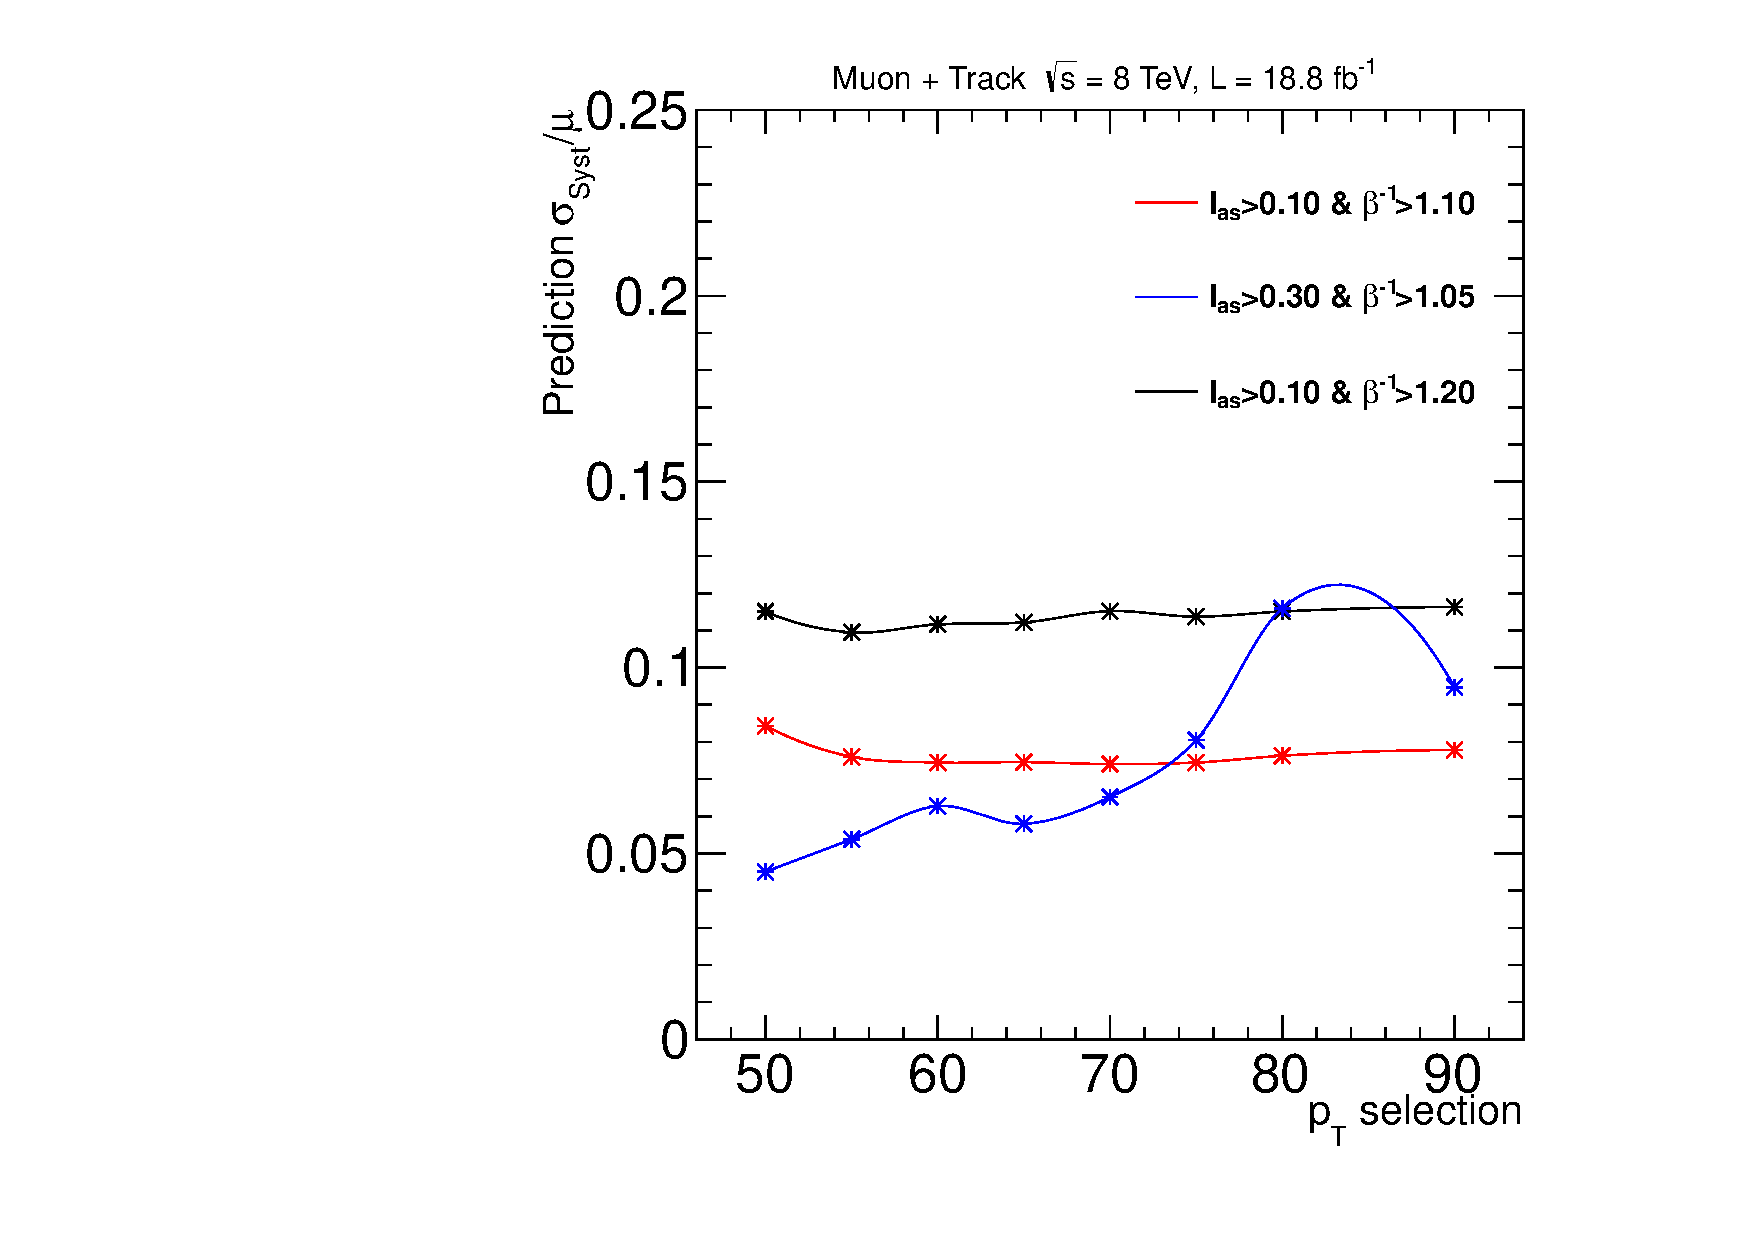
\includegraphics[clip=false, trim=0.0cm 0cm 0.0cm 0cm, width=0.48\textwidth]{figures/tkmu/Systematics_Data8TeV_pT_Syst}
\caption[Statistical and systematic uncertainty in the background prediction for different sets of thresholds in the \tktof\ analysis.]
{
Relative uncertainty on the background prediction in the \tktof\ analysis.
Three different sets of \invbeta\ and \dedx\ thresholds are plotted. Threshold on \pt\ set by the $x$-axis.
Plots show $S^{syst+stat}_{4}/\langle x \rangle$ (top left), $S^{stat}_{4}\langle x \rangle$ (top right), and $S^{syst}_{4}\langle x \rangle$ (bottom)
where $\langle x \rangle$ is the average predicted background.
The uncertainty variables are defined in Equation~\ref{eq:variance}.
%Calculation of uncertainty in the \tktof\ analysis.
%Top left: Ratio of the square root of the quadratic
%mean of the statistical uncertainties of the three possible background
%estimations to the mean of these estimations vs
%the $p_T$ threshold. Top right: Ratio of the standard deviation to the mean of the three
%background estimations vs $p_T$. Right: Ratio of the
%square root of the difference between the variance and the quadratic
%mean of the statistical uncertainties  of the three possible background
%estimations and the mean vs $p_T$.
}
\label{fig:TkMuUnc}
\end{center}
\end{figure}

\subsection{Prediction for \tkonly\ analysis}

The prediction for the \tkonly\ analysis is the same as the \tktof\ analysis except only the variables $p_T$ and \ias\ are used in a traditional two
dimensional ABCD method. 
The signal region, $D$, is predicted as $H \times B / F$ (see Table~\ref{tab:BinNames}).
The systematic uncertainty on the background prediction for the \tkonly\ analysis is taken as the same 20\% as in the \tktof\ analysis.
This is a conservative estimate as the \tkonly\ analysis uses only two of the three variables used in the \tktof\ analysis
and the correlation between three variables should be larger than for a subset of two of them.

\subsection{Prediction for \multi\ analysis}

The \multi\ analysis employs a two dimensional ABCD method using the variables \invbeta\ and \ias\ without a mass requirement. No mass requirement is applied as the mass
estimation assumes Q=1e and the large amount of saturation of the tracker readout (see Section~\ref{sec:otherpreselection}) prevents correcting for the charge.
%Once again the \invbeta\ less than one region can be used to perform systematic studies.
No \pt\ requirement above the one applied at preselection is used in the \multi\ analysis because the reconstructed \pt\ of
multiply charged particles is underestimated by a factor of 1/Q. This makes the separation between signal and background in the \pt\ spectrum small and a
higher threshold would remove similar fractions of signal and background.

The signal region, D, is predicted as $H \times C / G$ (see Table~\ref{tab:BinNames}).
The background prediction is checked by using 
the control region with \invbeta\ $< 1$ as was done for the \muononly\ analysis.
Figure~\ref{fig:MultiPred} shows the predicted and observed number of tracks for various \invbeta\ and \ias\ thresholds in the $D^{\prime}$ region: good agreement is observed.

\begin{figure}
 \begin{center}
%  \includegraphics[clip=false, trim=0.0cm 0cm 0.0cm 0cm, width=0.48\textwidth]{figures/multi/Prediction_Data8TeV_NPredVsNObsLinear_Flip}
  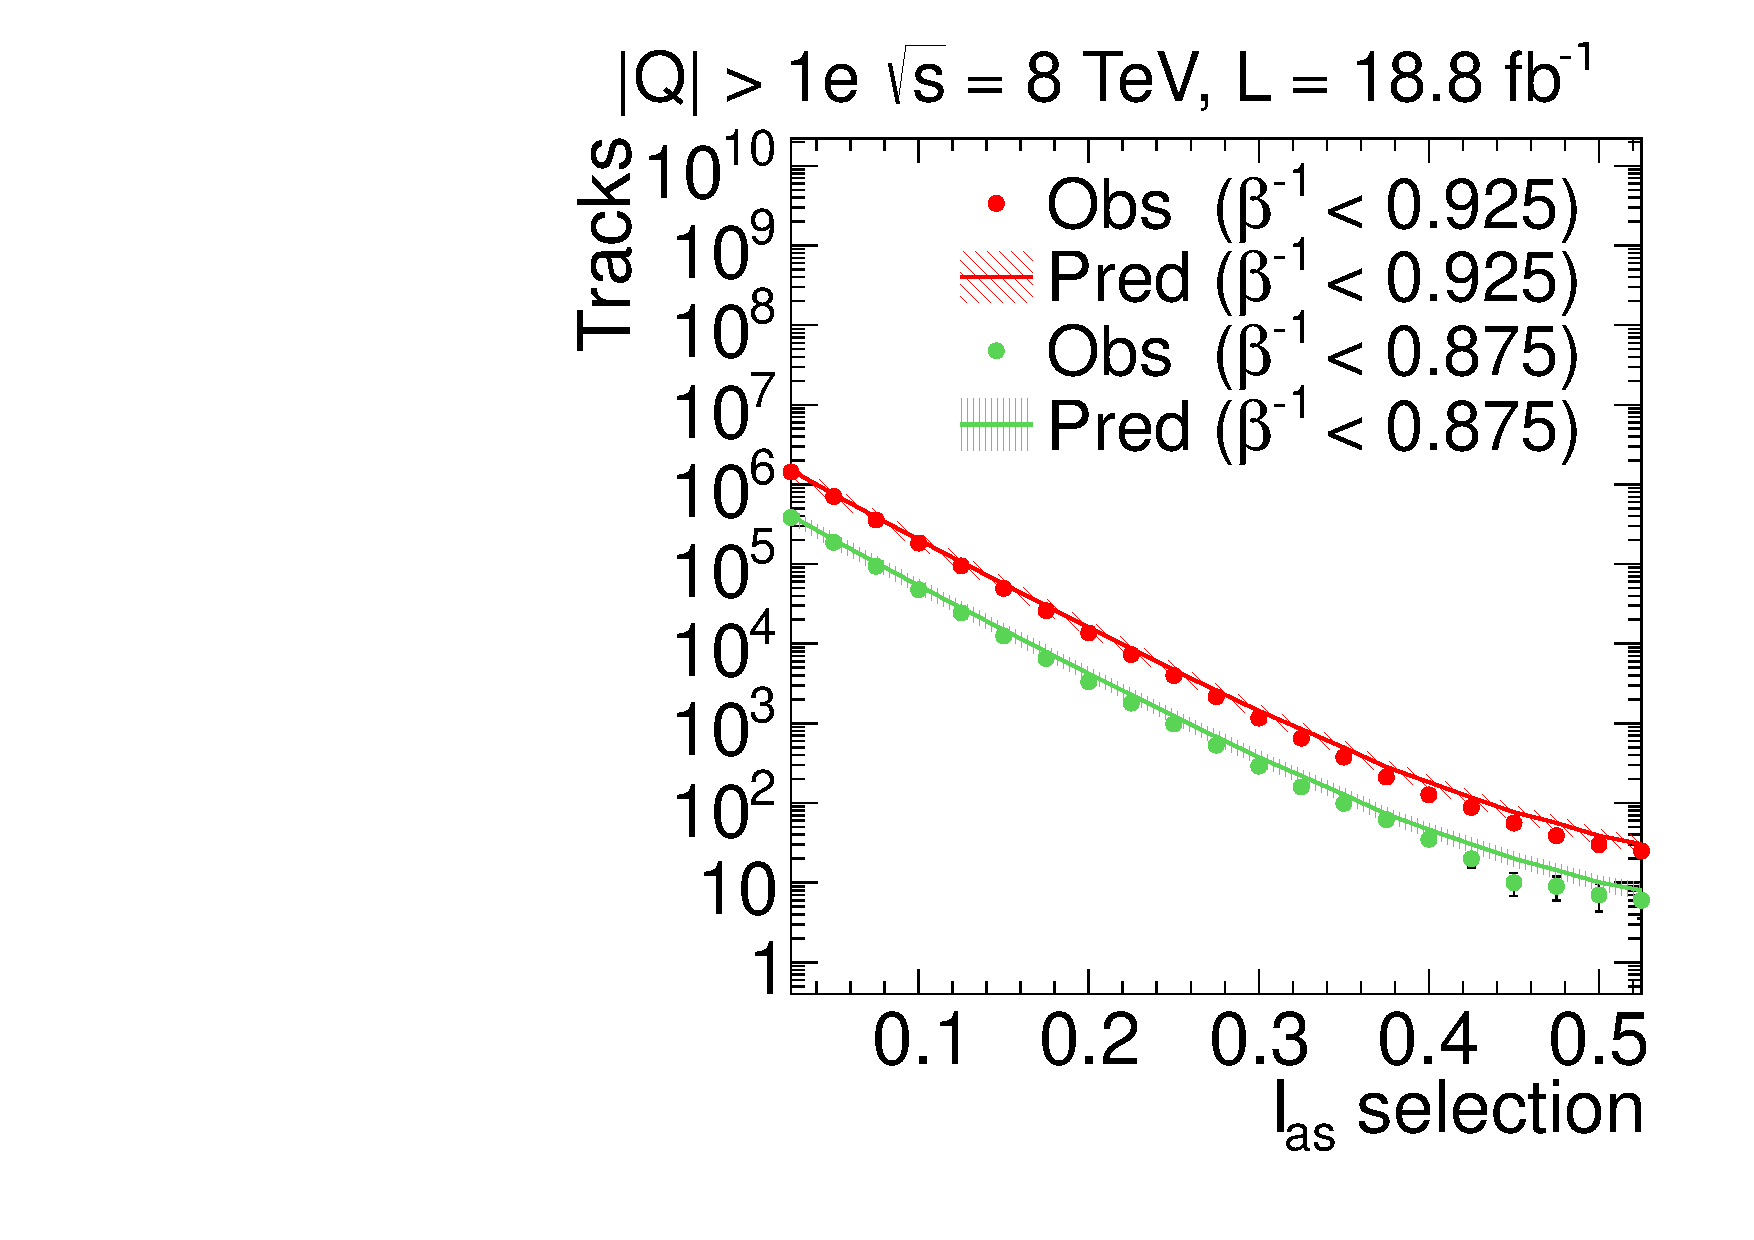
\includegraphics[clip=false, trim=0.0cm 0cm 0.0cm 0cm, width=0.48\textwidth]{figures/multi/Prediction_Data8TeV_NPredVsNObs_Flip}
 \end{center}
 \caption[Predicted and observed number of tracks in the \invbeta\ $<$ 1 region for different sets of thresholds in the \multi\ analysis.]
{Predicted and observed number of tracks in the \multi\ analysis in the $D^{\prime}$ region for different \invbeta\ thresholds with the x-axis indicating the \ias\ threshold.
Figure is cumulative, as tracks passing the selection with tight thresholds will also pass for loose thresholds.
}
\label{fig:MultiPred}
\end{figure}

The systematic uncertainty for the \multi\ analysis is determined by the same method as the \muononly\ analysis except replacing \pt\ for \ias. 
Two additional predictions are made using the tracks in the \invbeta\ $< 1$ region.
Figure~\ref{fig:mCHAMPcorr} shows the predicted number of tracks for various \invbeta\ and \dedx\ thresholds for the three predictions.

\begin{figure}%[tbhp!]
 \begin{center}
 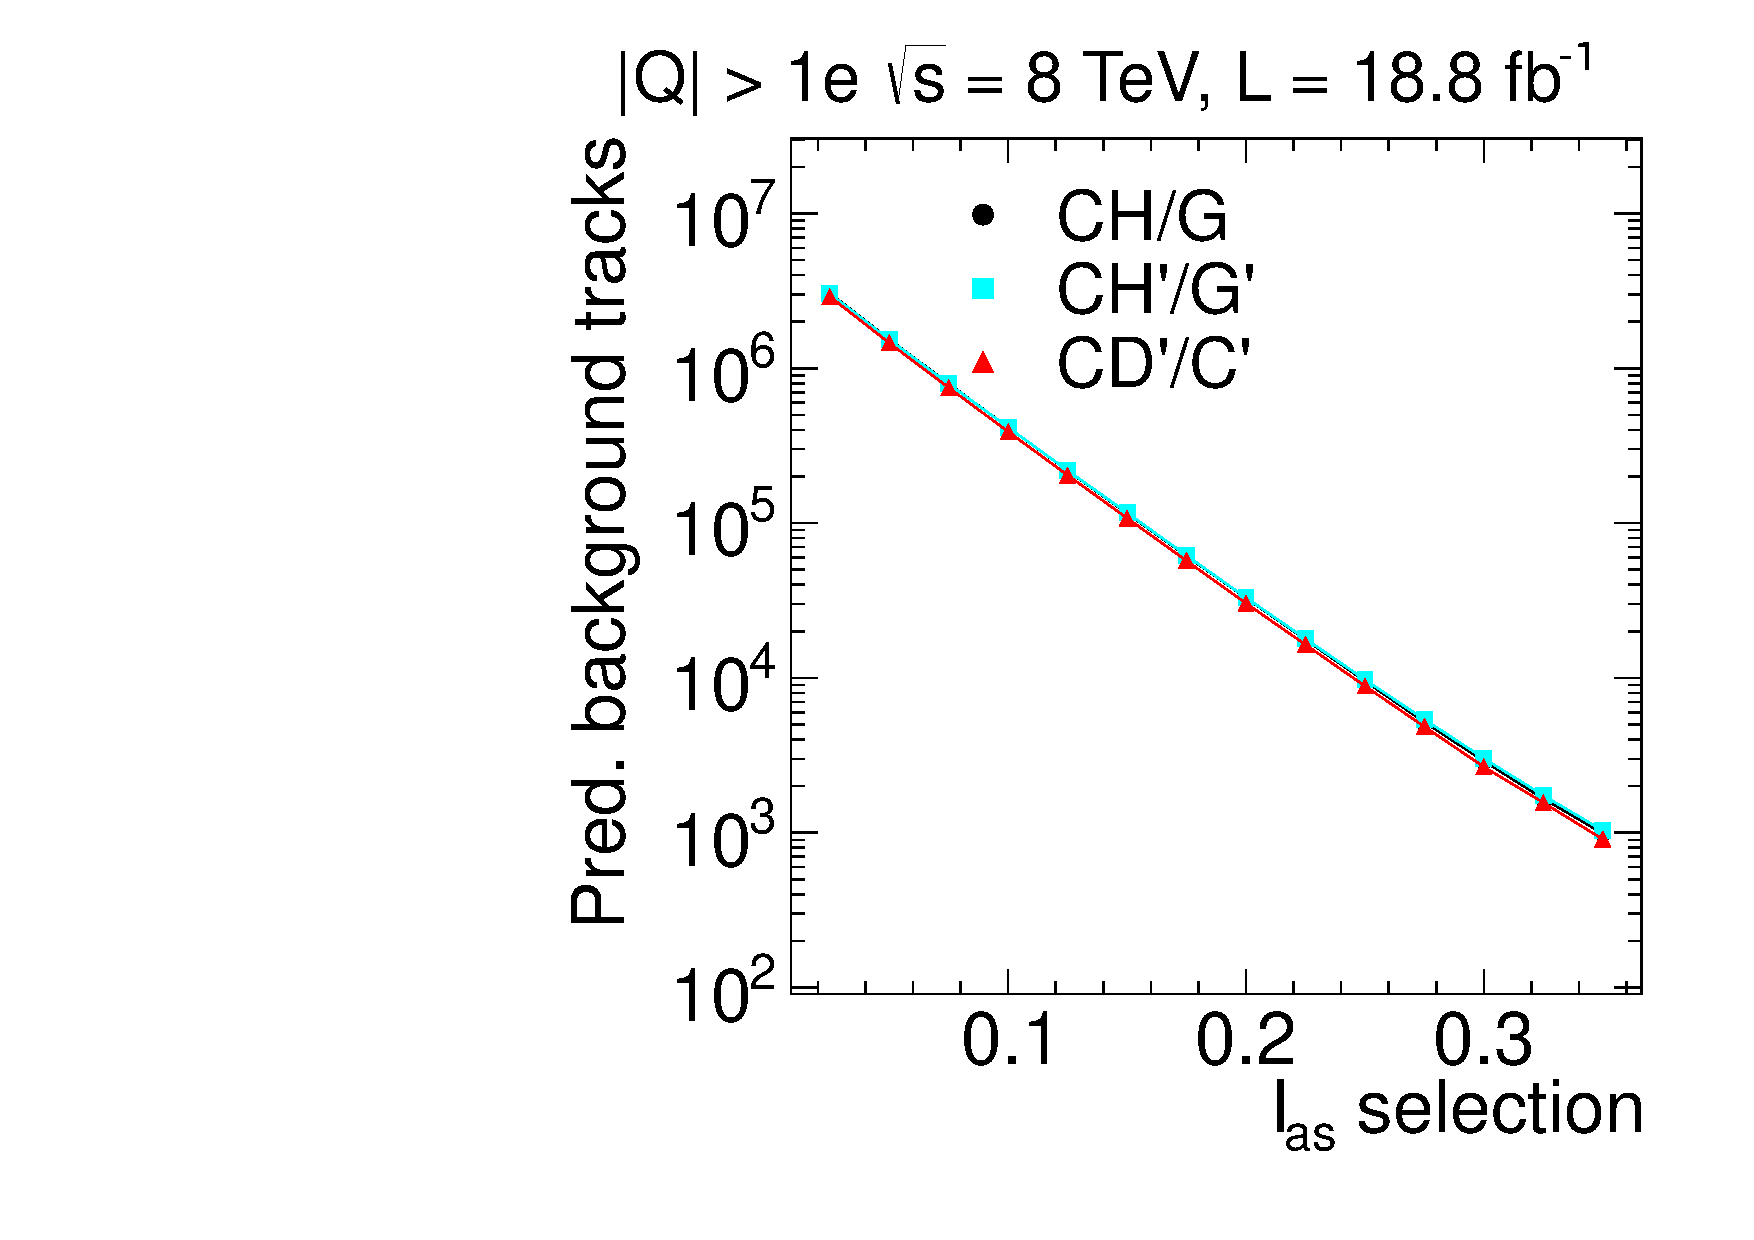
\includegraphics[clip=false, trim=0.0cm 0cm 0.0cm 0cm, width=0.48\textwidth]{figures/multi/Data8TeVCollisionPrediction_TOF105}
 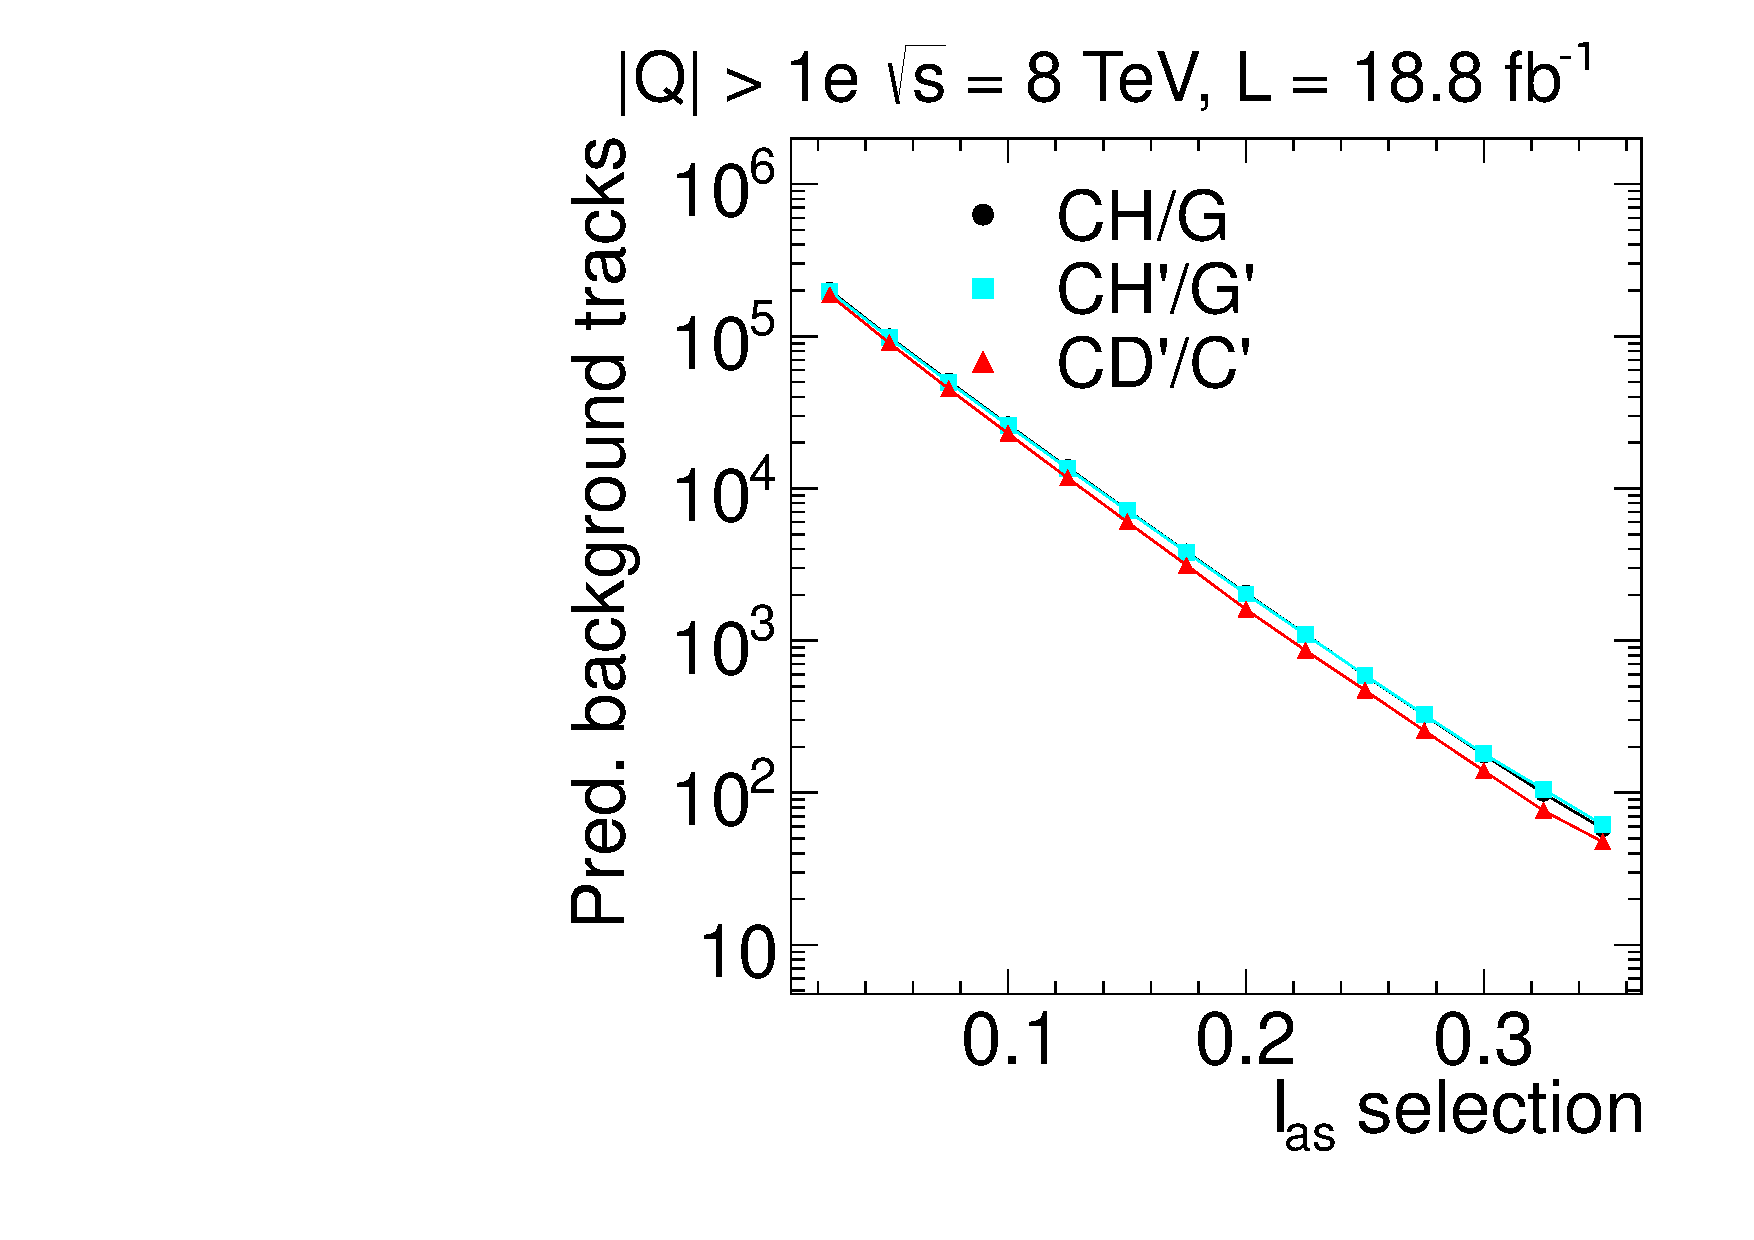
\includegraphics[clip=false, trim=0.0cm 0cm 0.0cm 0cm, width=0.48\textwidth]{figures/multi/Data8TeVCollisionPrediction_TOF115}
 \end{center}
 \caption[Distribution of the number of predicted tracks from different predictions in the \multi\ analysis]
{Distribution of the number of predicted tracks and their
   statistical error computed for the \multi\ analysis using
   different regions for two values of the $1/\beta$ threshold. The \ias\ threshold is defined by the x-axis.
Figures are cumulative, as tracks passing the selection with tight thresholds will also pass for loose thresholds.
Left: $1/\beta>1.05$ ($<0.95$ for low $1/\beta$ regions). Right: $1/\beta>1.15$ ($<0.85$ for low $1/\beta$ regions).}
 \label{fig:mCHAMPcorr}
\end{figure}

The spread in the three predictions is then used to determine the systematic uncertainty through Equation~\ref{eq:variance} with N=3.
Fig.~\ref{fig:mCHAMPcorr2} shows the variation of the statistical and systematic uncertainties as a function of the $I_{as}$ threshold.
From the last plot a 20\% systematic uncertainty is taken on the background estimate for the \multi\ analysis.

\begin{figure}
 \begin{center}
 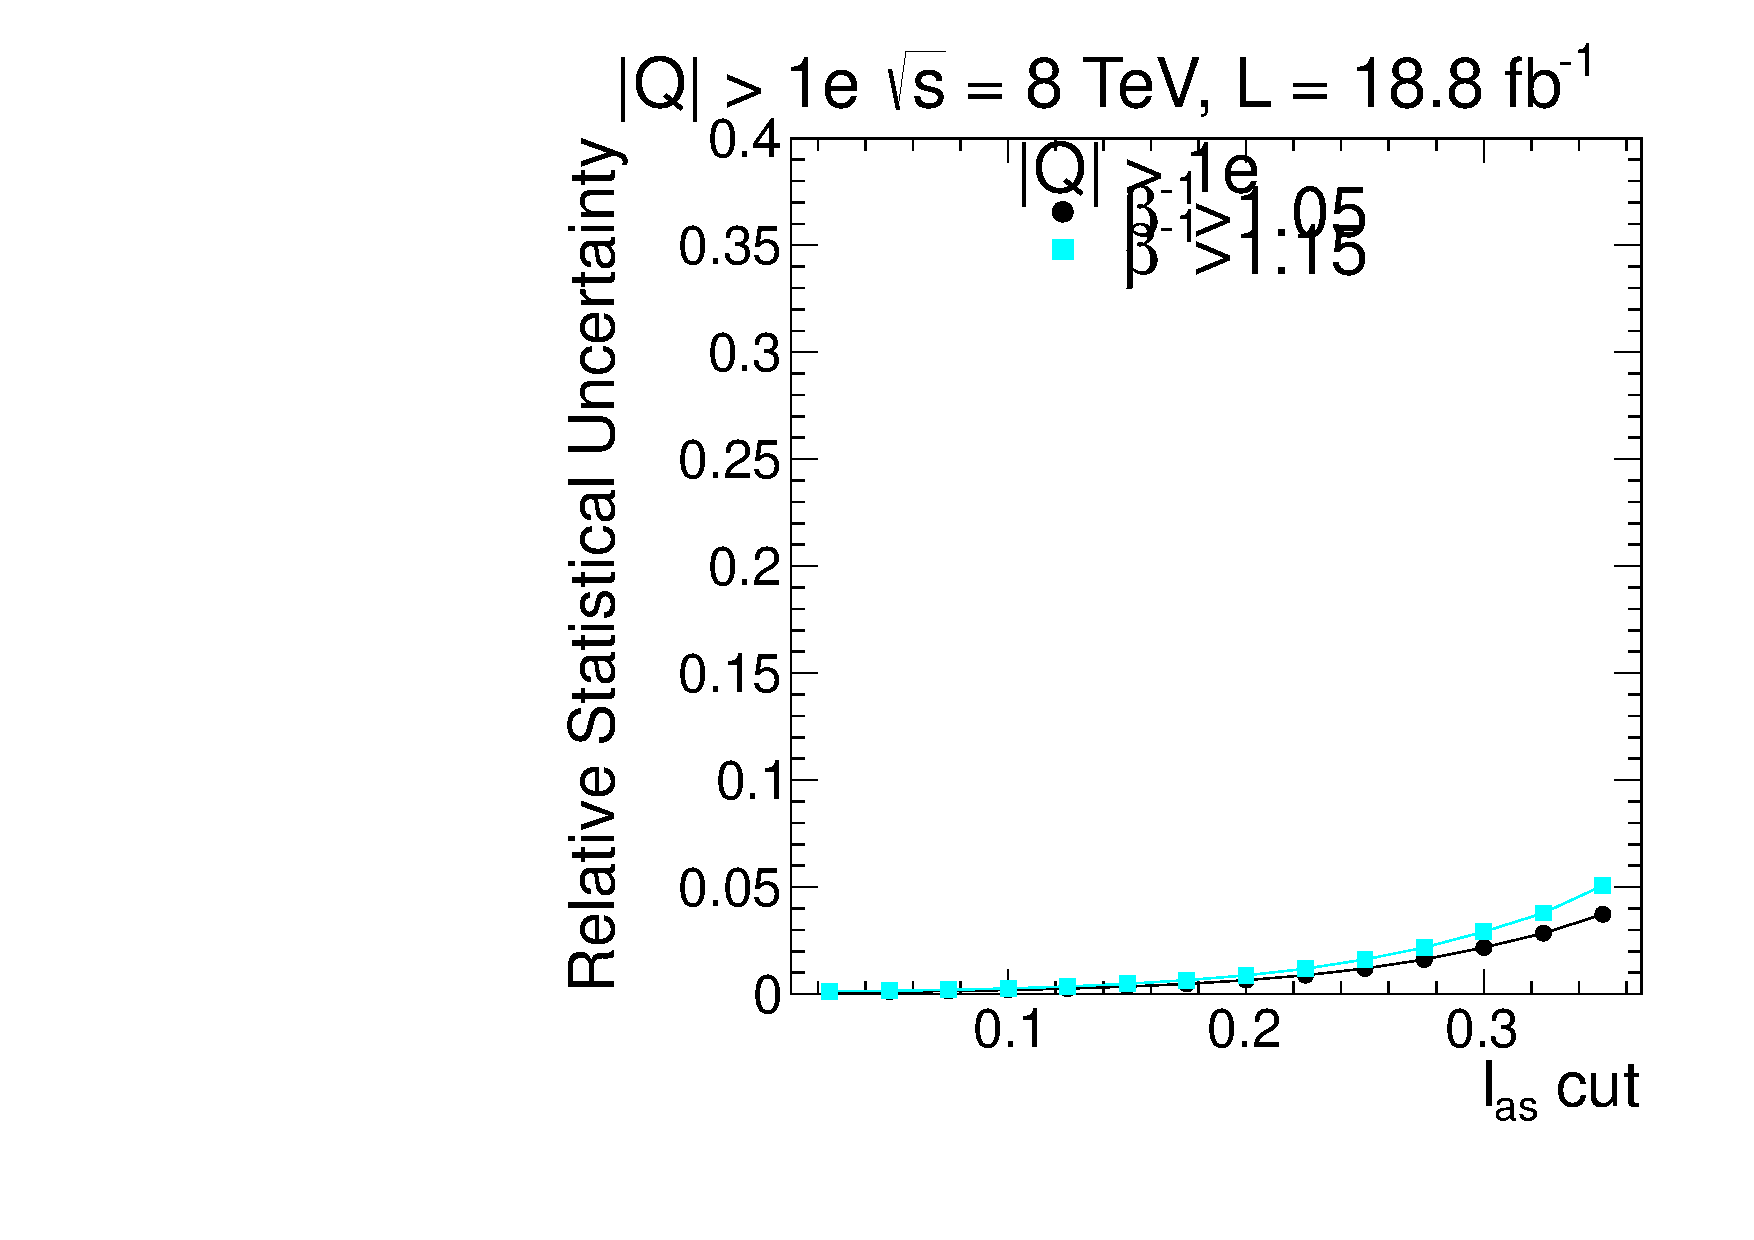
\includegraphics[clip=false, trim=0.0cm 0cm 0.0cm 0cm, width=0.48\textwidth]{figures/multi/Data8TeVCollisionStat}
 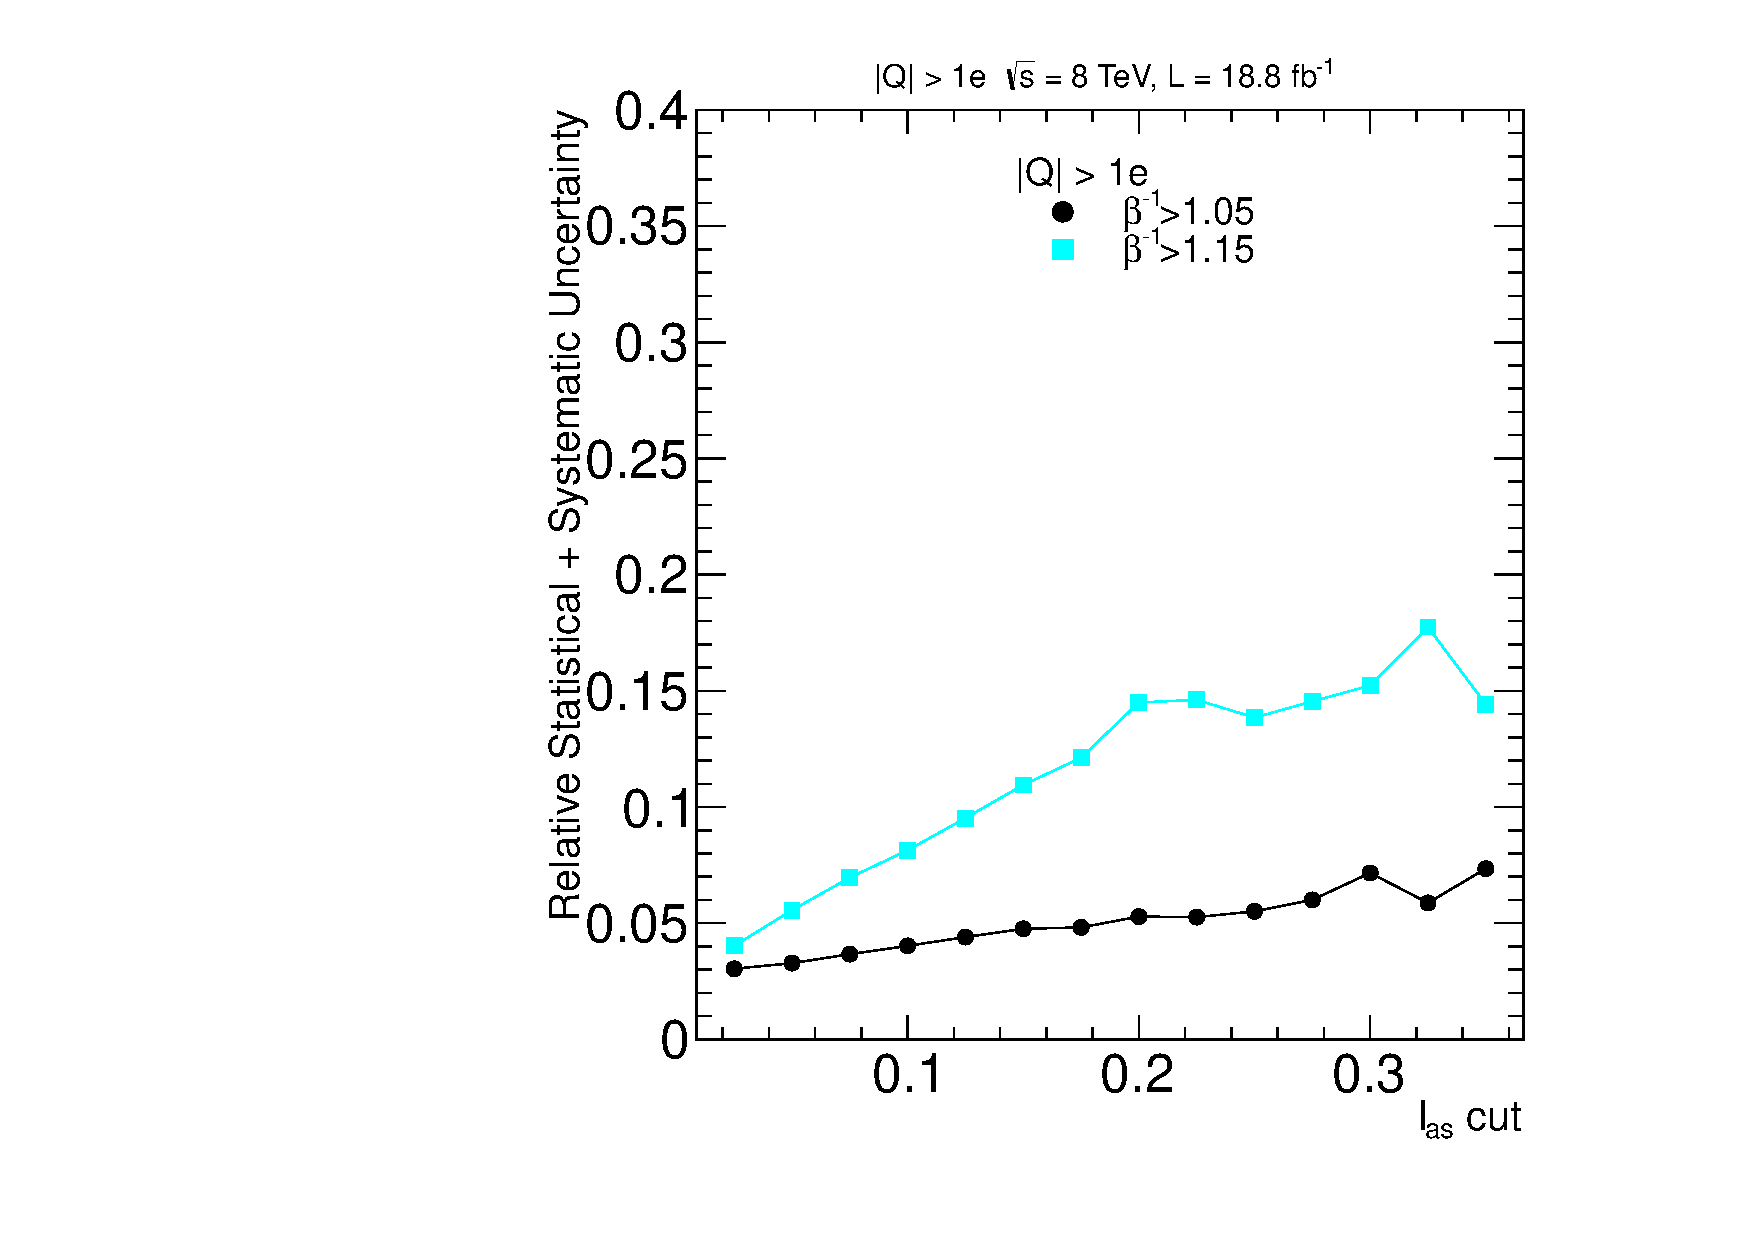
\includegraphics[clip=false, trim=0.0cm 0cm 0.0cm 0cm, width=0.48\textwidth]{figures/multi/Data8TeVCollisionStatSyst} \\
 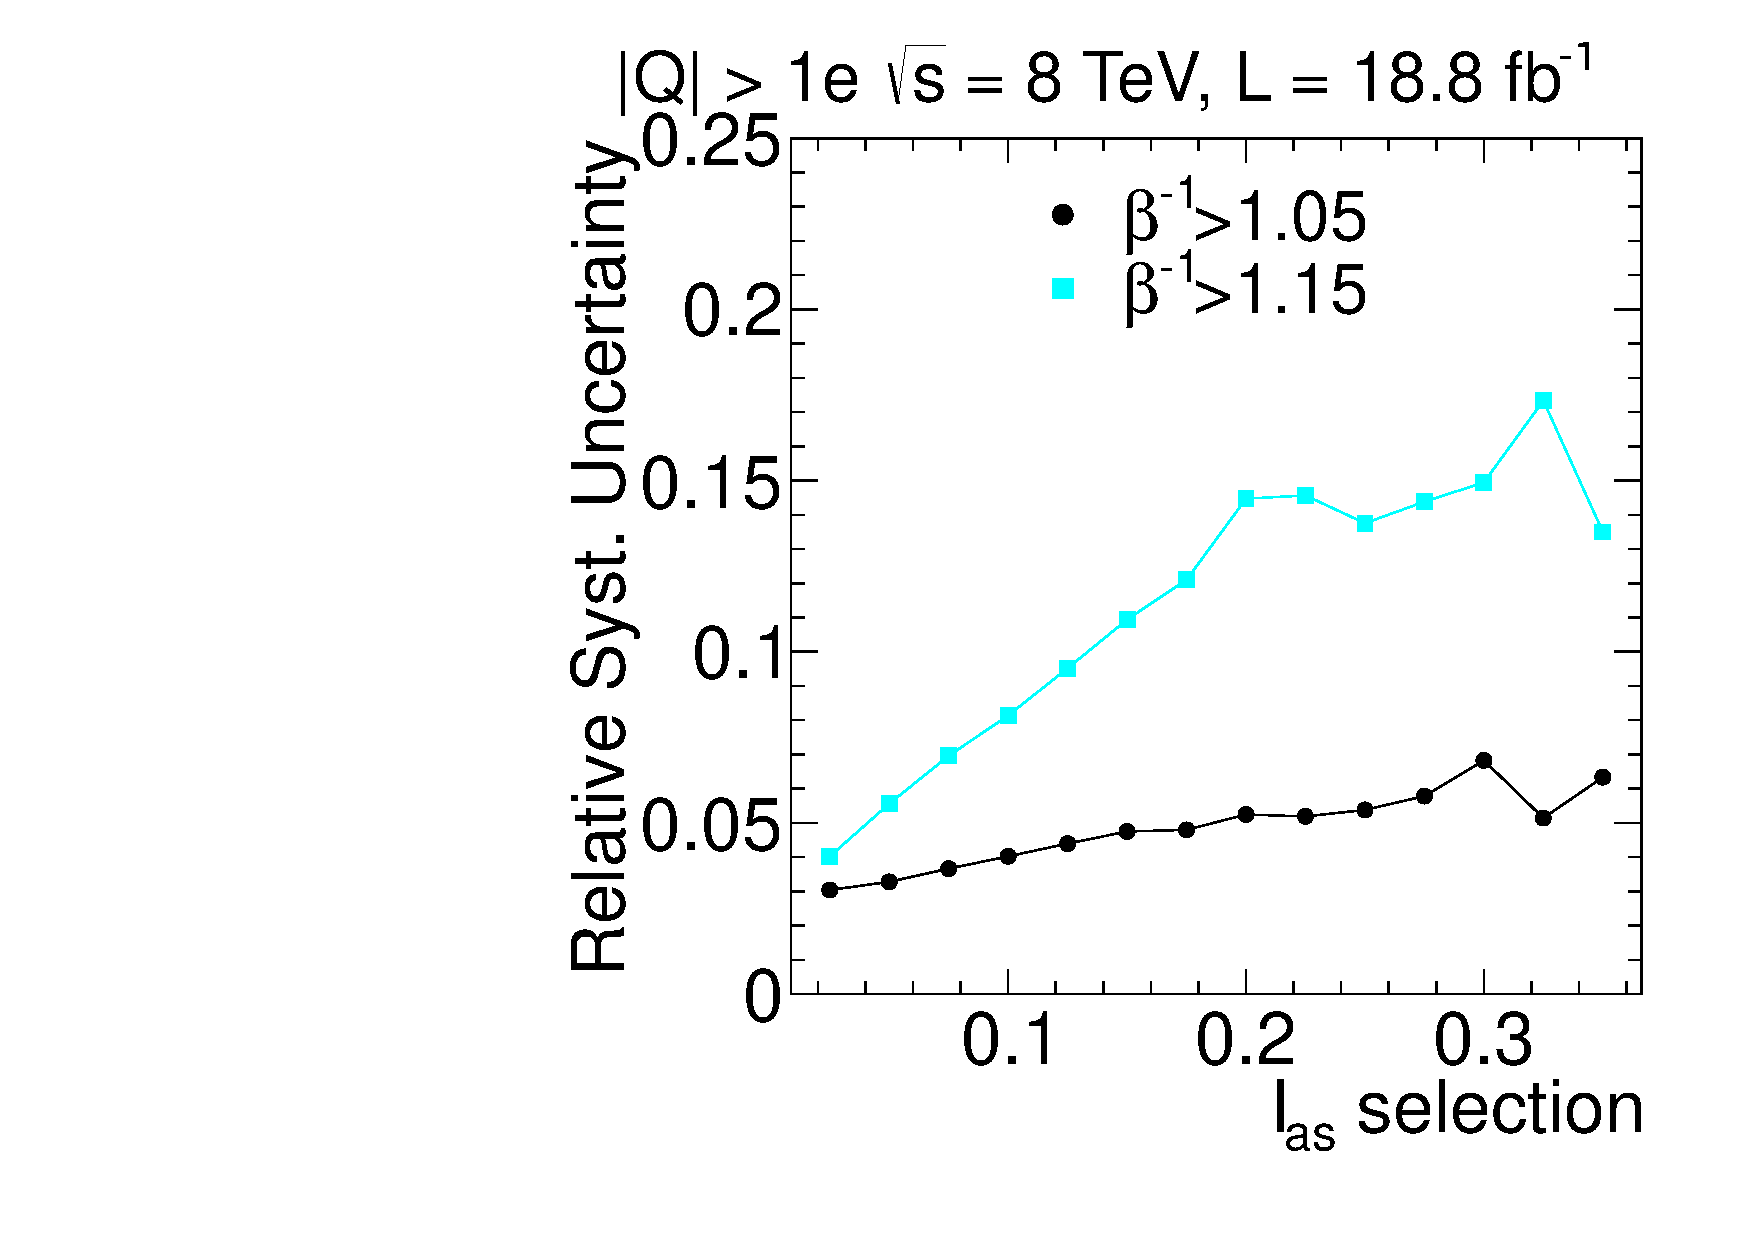
\includegraphics[clip=false, trim=0.0cm 0cm 0.0cm 0cm, width=0.48\textwidth]{figures/multi/Data8TeVCollisionSyst}
\end{center}
\caption[Statistical and systematic uncertainty in the background prediction for different sets of thresholds in the \multi\ analysis]
{
Relative uncertainty on the background prediction in the \multi\ analysis.
Two different \invbeta\ thresholds are plotted. Threshold on \ias\ set by the $x$-axis.
Plots show $S^{syst+stat}_{3}/\langle x \rangle$ (top left), $S^{stat}_{3}\langle x \rangle$ (top right), and $S^{syst}_{3}\langle x \rangle$ (bottom)
where $\langle x \rangle$ is the average predicted background.
The uncertainty variables are defined in Equation~\ref{eq:variance}.
%Calculation of uncertainty in the \multi\ analysis.
%Top left: Ratio of the square root of the quadratic
%mean of the statistical uncertainties of the three possible background
%estimations to the mean of these estimations vs
%the \ias\ threshold. Top right: Ratio of the standard deviation to the mean of the three
%background estimations vs \ias. Right: Ratio of the
%square root of the difference between the variance and the quadratic
%mean of the statistical uncertainties  of the three possible background
%estimations and the mean vs \ias.
}
\label{fig:mCHAMPcorr2}
\end{figure}
